

\NeedsTeXFormat{LaTeX2e}
%-----------------------------------------------------------
\documentclass[a4paper,12pt]{pkg/monografia}
\usepackage{makecell}
\usepackage[pdfpagelabels]{hyperref}
\usepackage[brazil]{babel}
\usepackage{minted}
\usepackage[utf8]{inputenc}
\usepackage{verbatimbox}
\usepackage{listings}
\usepackage{url, fancyhdr, amsmath,amsthm,amsfonts,amssymb, latexsym, bm}
\usepackage{array,booktabs,tablefootnote,multirow,xfrac,nicefrac,cite,array,enumitem,hhline}
\usepackage{graphicx,textcase,textcomp, glossaries, caption}
\usepackage[mathcal]{eucal}
\usepackage[alf]{pkg/abntcite}
\usepackage[portuguese,linesnumbered,boxruled,noend]{algorithm2e}
\usepackage{acronym}
\usepackage[table]{xcolor} 
\usepackage{float}
\usepackage{enumitem}
\usepackage{footnote}
\usepackage{tabularx}
\usepackage{subcaption}
\usepackage{glossaries}
\renewcommand*{\UrlFont}{\footnotesize}

\makesavenoteenv{table}
\makesavenoteenv{tabular}
\newlist{longenum}{enumerate}{5}
\setlist[longenum,1]{label=\roman*)}
\setlist[longenum,2]{label=\alph*)}
\setlist[longenum,3]{label=\arabic*)}
\setlist[longenum,4]{label=(\roman*)}
\setlist[longenum,5]{label=(\alph*)}


%%%%%%%%%% Lista de novos comandos %%%%%%%%%%
\newcommand{\blk}{\cellcolor{black}}
\newcommand{\mr}[3]{\multirow{#1}{#2}{#3}}
\newcommand{\mc}[3]{\multicolumn{#1}{#2}{#3}}
\newcommand{\mcbf}[3]{\multicolumn{#1}{#2}{\textbf{#3}}}
\newcommand{\mmbf}[3]{\multicolumn{2}{|#2|}{\textbf{#3}}}

\renewcommand\qedsymbol{$\blacksquare$}

\newtheorem{definition}{Definição}
\newtheorem{theorem}{Teorema}[section]
\newtheorem{corollary}{Corolário}[theorem]
\newtheorem{lemma}[theorem]{Lema}

\newtheoremstyle{sltheorem}
{}                % Space above
{}                % Space below
{}                % Theorem body font % (default is "\upshape")
{}                % Indent amount
{\bfseries}       % Theorem head font % (default is \mdseries)
{:}               % Punctuation after theorem head % default: no punctuation
{ }               % Space after theorem head
{}                % Theorem head spec
\theoremstyle{sltheorem}
\newtheorem{exemplo}{Exemplo}
\newtheorem{contraexemplo}{Contra-Exemplo}

%comentários e anotações da karina
\newcommand{\comentando}[1]{\textcolor{red}{#1}}

\SetNlSty{textbf}{}{:}
\setlength{\algomargin}{2.5em}


\hypersetup{
    unicode      = false, 
    pdftoolbar   = false,	
    pdfmenubar   = false,	
    pdffitwindow = true,	
    pdfstartview = {FitH},
    pdftitle     = {Mecanismo de Criptografia Pós-Quântica ML-KEM: Uma Introdução para Estudantes de Ciência da Computação},
    pdfauthor    = {Wallace Mielniczki},	
    pdfsubject   = {Trabalho de Conclusão de Curso - II},  
    pdfcreator   = {Mielniczki, W.},
    pdfproducer  = {Mielniczki, W.},	
    pdfkeywords  = {}, 
    pdfnewwindow = true,	
    colorlinks   = true,	
    linkcolor    = black,	
    citecolor    = black,	
    filecolor    = blue,
    urlcolor     = black
}
\makeglossaries
%-----------------------------------------------------------
%-----------------------------------------------------------
\begin{document}
%
%----------------- Título e Dados do Autor -----------------
\titulo{Mecanismo de Criptografia Pós-Quântica ML-KEM: Uma Introdução para Estudantes de Ciência da Computação}%
\autor{Wallace Mielniczki}%
\nome{Wallace Mielniczki}%
\ultimonome{Mielniczki}%
%
%---------- Informe o Curso e Grau -----
\bacharelado \curso{Ciência da Computação} \mes{Dezembro} \ano{2023} 
\data{\today}% data da aprovação
\cidade{Joinville}%
%
%----------Informações sobre a Institução -----------------
\instituicao{Universidade do Estado de Santa Catarina}%
\sigla{UDESC}% 
\unidadeacademica{Centro de Ciências Tecnológicas}%
%
\orientador{Karina Girardi Roggia}%
%    
\examinadorum{Debora Cabral Nazário}%
%
\examinadordois{Charles Christian Miers}%
%
\examinadortres{Rafael Rodrigues Obelheiro}%
%

%---------------------------------------------------------------%
%--------- Títulos do Orientador 1o. e 2o. Examinadores ----
\ttorientador{Doutora}%
\ttexaminadorum{Doutora}%
\ttexaminadordois{Doutor}
\ttexaminadortres{Doutor}

\hypersetup{pageanchor=false}
\maketitle
\hypersetup{pageanchor=true}

%--------Digite aqui o seu resumo em Português--------------
\resumo{Resumo}
\noindent
Em 1994, Peter Shor apresentou um algoritmo que resolve o problema da fatoração de números inteiros e do logaritmo discreto em tempo polinomial por um computador quântico, tais problemas são a base da segurança de algoritmos de criptografia assimétrica amplamente utilizados, tais como RSA e ECDH. Com o avanço nas pesquisas na área da computação quântica, iniciou-se uma preocupação com relação à segurança dos dados que dependem de sistemas criptográficos comprometidos pelo algoritmo de Shor. Em 2016, o \textit{National Institute of Standards and Technology} (NIST) iniciou o programa \textit{Post-Quantum Cryptography Standardization}, cujo objetivo é selecionar algoritmos de criptografia assimétricos e de assinatura digital resistentes a ataques realizados por computadores clássicos e quânticos, que possam ser utilizados em computadores convencionais. Dentre os algoritmos selecionados para padronização em 2022, está o algoritmo \ac{ML-KEM} para criptografia assimétrica, que é abordado nesse trabalho. Este trabalho visa servir como um material de estudos para acadêmicos de ciência da computação sobre o algoritmo \ac{ML-KEM} e sua relação com reticulados.\\

\noindent
\textbf{Palavras-chave:} criptografia, criptografia assimétrica, criptografia pós-quântica, reticulados.


%-----------Digite aqui o seu resumo em Inglês--------------
\resumo{Abstract}
\noindent
In 1994 Peter Shor presented an algorithm that solves the factorization problem of integers and the discrete logarithm in polynomial time by a quantum computer, such problems are the basis of the security of widely used asymmetric cryptography algorithms, such as RSA and ECDH. Due to quantum computing research advances, a concern has arisen regarding the security of data that depend on cryptographic systems compromised by Shor's algorithm. In 2016, the National Institute of Standards and Technology (NIST) started the Post-Quantum Cryptography Standardization program, whose objective is to select asymmetric cryptography and digital signature algorithms resistant to attacks performed by classical and quantum computers, which can be used in conventional computers. Among the algorithms selected for standardization in 2022 is the Module-Lattice-based Key-Encapsulation Mechanism (ML-KEM) algorithm for asymmetric cryptography that will be addressed in this work. This work aims to serve as a study material on the ML-KEM algorithm and its relation to lattices, for computer science academics.\\

\noindent
\textbf{Keywords:} cryptography, asymmetric cryptography, post-quantum cryptography, lattices.

%-----------------------------------------------------------

\thispagestyle{empty} 
\listoffigures
\listofabbreviations{Lista de Abreviaturas} % lista de abreviações
\begin{acronym} 
    \acro{CRYSTALS}{{\it Cryptographic Suite for Algebraic Lattices}}
    \acro{CVP}{{\it Closest Vector Problem}}
    \acro{DSA}{{\it Digital Signature Algorithm}}
    \acro{ECC}{{\it Elliptic-curve cryptography}}
    \acro{ECDH}{{\it Elliptic-curve Diffie–Hellman}}
    \acro{ECDSA}{{\it Elliptic Curve Digital Signature Algorithm}}
    \acro{GapSVP}{{\it Gap Shortest Vector Problem}}
    \acro{GNFS}{{\it General Number Field Sieve}}
    \acro{KEM}{{\it Key-Encapsulation Mechanism}}
    \acro{LWE}{{\it Learning With Errors}}
    \acro{ML-KEM}{{\it Module-Lattice-based Key-Encapsulation Mechanism}}
    \acro{MLWE}{{\it Module Learning With Errors}}
    \acro{NIST}{{\it National Institute of Standards and Technology}}
    \acro{NP-HARD}{{\it Non-deterministic Polynomial-time Hardness}}
    \acro{NTT}{{\it Number Theoretic Transform}}
    \acro{PQC}{{\it Post-Quantum Cryptography}}
    \acro{RLWE}{{\it Ring Learning With Errors}}
    \acro{RSA}{{\it Rivest-Shamir-Adleman}}
    \acro{SIVP}{{\it Shortest Independent Vector Problem}}
    \acro{SVP}{{\it Shortest Vector Problem}}
\end{acronym} 
\printglossary

%-----------------------------------------------------------

%----Sumário, lista de figura e de tabela ------------
\listoftables
\tableofcontents 
\thispagestyle{empty}
\newpage

%--------------Início do Conteúdo---------------------------
\pagestyle{ruledheader}

\definecolor{mGreen}{rgb}{0,0.6,0}
\definecolor{mGray}{rgb}{0.5,0.5,0.5}
\definecolor{mPurple}{rgb}{0.58,0,0.82}
\definecolor{backgroundColour}{rgb}{0.95,0.95,0.92}

\chapter{Introdução} 
\label{chap:intro}

Em 1994 Peter Shor apresentou um algoritmo que resolve o problema da fatoração de números inteiros e do logaritmo discreto em tempo polinomial por um computador quântico \cite{shor}, tais problemas são a base da segurança de algoritmos de criptografia assimétrica amplamente utilizados, como \ac{RSA} e \ac{ECDH}. Algumas empresas como IBM, Microsoft, Intel e Google estão investindo fortemente na pesquisa de computadores quânticos e tecnologias relacionadas. Em 2019 o Google anunciou a conquista da supremacia quântica, quando um computador quântico supera em alguma tarefa um computador clássico, resolvendo um problema em 200 segundos em que um supercomputador clássico resolveria em aproximadamente 10000 anos \cite{google}. Uma equipe de pesquisadores da China fatorou uma chave de 48 bits usando um computador quântico de 10 qubit, a equipe estimou fatorar uma chave de 2048 bits com um computador de 372 qubits usando seu algoritmo\cite{yan2022factoring}, entretanto a IBM já possui um computador quântico com um processador de 433 qubit \cite{ibm433qubit}.

Com o avanço nas pesquisas na área da computação quântica, iniciou-se uma preocupação com relação à segurança dos dados que dependem de sistemas criptográficos comprometidos pelo algoritmo de Shor. Em 2016 o \ac{NIST} iniciou o programa \textit{Post-Quantum Cryptography Standardization}, cujo objetivo é selecionar algoritmos de criptografia assimétricos e de assinatura digital resistentes a ataques realizados por computadores clássicos e quânticos, que possam ser utilizados em computadores convencionais \cite{nist}. Os algoritmos participantes são estudados e avaliados pela comunidade científica, considerando a segurança, eficiência e interoperabilidade com outros protocolos de criptografia atuais. O processo de padronização é realizado em rodadas, os algoritmos mais promissores são selecionados para prosseguir para a próxima rodada. 

Na primeira rodada foram submetidos 45 esquemas de criptografia assimétrica e 19 de assinatura digital. A Tabela \ref{tab:nist_pqc_round_1} mostra os diferentes tipos de criptografia assimétrica e de assinatura digital submetidos nessa rodada do programa, dos quais após 3 rodadas foram selecionados para padronização e substituição em larga escala os algoritmos mostrados na Tabela \ref{tab:nist_pqc_selected}. Outros algoritmos prosseguiram para a quarta rodada, na qual continuam sendo estudados e avaliados para uma possível padronização futuramente. Embora os algoritmos baseados em reticulados apresentem uma ótima segurança e desempenho, não se é recomendado depender apenas de um tipo de criptografia, este é o motivo da padronização do algoritmo SPHINCS+ e do estudo dos algoritmos da quarta rodada, conforme pode ser observado na Tabela \ref{tab:nist_pqc_four_round}.

    \begin{table}[h]
        \centering
        \caption{Primeira rodada do NIST PQC.}
        \begin{tabular}{|c|c|c|}
            \hline
            Tipo & Criptografia assimétrica & Assinatura digital \\ \hline
            Baseada em reticulados & 21 & 5 \\ \hline
            Baseada em código    & 17 & 2 \\ \hline
            Baseada em \textit{hash}    & 0  & 3 \\ \hline
            Multivariada  & 2  & 7 \\ \hline
            Outros        & 5  & 2 \\ \hline
        \end{tabular}\\
        \footnotesize{Fonte: Adaptado de: \cite{nist_round1}.}
        \label{tab:nist_pqc_round_1}
    \end{table}

    \begin{table}[h]
        \centering
        \caption{Algoritmos selecionados do NIST PQC.}
        \begin{tabular}{|c|c|c|}
            \hline
            Tipo & Criptografia assimétrica & Assinatura digital        \\ \hline
            Baseada em reticulados & CRYSTALS-Kyber & \begin{tabular}[c]{@{}c@{}}CRYSTALS-Dilithium\\ FALCON\end{tabular} \\ \hline
            Baseada em \textit{hash}    &                & SPHINCS+                   \\ \hline
        \end{tabular}\\
        \footnotesize{Fonte: Adaptado de: \cite{nist_round1}.}
        \label{tab:nist_pqc_selected}
    \end{table}

    \begin{table}[!htbp]
        \centering
        \caption{Quarta rodada do NIST PQC.}
        \begin{tabular}{|c|c|}
            \hline
            Tipo & Criptografia assimétrica                                        \\ \hline
            Baseada em código                             &\begin{tabular}[c]{@{}c@{}}BIKE\\ Classic MacEliece\\ HQC\end{tabular} \\ \hline
            Baseada em isogenia    & SIKE                         \\ \hline
        \end{tabular}\\
        \footnotesize{Fonte: Adaptado de: \cite{nist_round1}.}
        \label{tab:nist_pqc_four_round}
    \end{table}

A equipe \ac{CRYSTALS} desenvolveu dois sistemas criptográficos, escolhidos para padronização após avaliações da comunidade científica no programa \textit{Post-Quantum Cryptography Standardization} do \ac{NIST}, sendo o algoritmo Kyber para criptografia de chave assimétrica e Dilithium para assinatura digital \cite{nist3}. Após a aprovação e padronização do Kyber no programa PQC em 24 de agosto de 2023, o \ac{NIST} alterou o nome do algoritmo Kyber para \ac{ML-KEM}. O algoritmo \ac{ML-KEM}, que é o foco deste trabalho, é baseado no esquema \ac{LWE} introduzido por \cite{regev}, tal modelo ficou famoso devido a sua relação com alguns problemas de difícil resolução baseados em reticulados, como \ac{SVP} e \ac{CVP}, que possuem grande complexidade de resolução mesmo para um computador quântico.

Devido ao fato da popularidade da criptografia baseada em reticulados ser recente, existe uma escassez de materiais didáticos acessíveis destinados a estudantes de ciência da computação interessados no algoritmo \ac{ML-KEM} e nos conceitos matemáticos associados. O propósito deste trabalho é fornecer um material de estudo de fácil compreensão que aborda o algoritmo de criptografia pós-quântico \ac{ML-KEM} e os princípios matemáticos subjacentes, tornando-os acessíveis a estudantes de computação. Os objetivos específicos deste trabalho incluem:

\noindent
\begin{itemize}
    \item Apresentar uma introdução à criptografia, contextualizando seus diversos tipos;
    \item Explorar os conceitos de reticulados e suas aplicações na criptografia, fornecendo uma base sólida para compreensão;
    \item Especificar e compreender os principais problemas computacionais envolvendo reticulados;
    \item Oferecer todos os conceitos para o entendimento do algoritmo \ac{ML-KEM} de forma simplificada. 
    \item Realizar uma implementação simplificada do algoritmo \ac{ML-KEM}.
\end{itemize}

A implementação simplificada na linguagem C do algoritmo ML-KEM pode ser encontrada no repositório do GitHub em \url{https://github.com/opallace/ML-KEM}.

O desenvolvimento deste trabalho se deu por meio de uma pesquisa referenciada e aplicada, com o uso de diversas pesquisas pré-existentes como base teórica para o desenvolvimento do texto apresentado neste documento.

A estrutura do texto consiste em cinco capítulos, no qual o primeiro capítulo introduz o problema, motivação e os objetivos deste trabalho. O Capítulo \ref{cap:criptografia} apresenta alguns conceitos básicos de criptografia e criptoanálise, fundamentais para o entendimento da área. No Capítulo \ref{cap:reticulados} é abordada a estrutura algébrica de reticulados, que possui problemas computacionais que compõem a base da segurança do algoritmo \ac{ML-KEM}. A explicação do algoritmo \ac{ML-KEM} está no Capítulo \ref{cap:ml_kem}, sendo que, na Seção \ref{sec:k-pke} é explicado o algoritmo K-PKE, utilizado como um subprocesso do \ac{ML-KEM}. Por fim, seguem-se as conclusões e trabalhos futuros abertos a partir deste no Capítulo \ref{cap:consideracoes_parciais}. Podem ser encontrados, nos apêndices, os conceitos, demonstrações matemáticas e os algoritmos abordados.
\chapter{Criptografia}
\label{cap:criptografia}

A criptologia é a ciência das comunicações secretas \cite{history_of_cryptography_and_cryptanalysis} que contempla diversas técnicas para garantir uma comunicação segura entre um emissor e seu destinatário, através de um canal de comunicação suscetível a interceptações por terceiros não autorizados. A criptologia possui três subáreas: esteganografia, criptografia e criptoanálise. A esteganografia visa ocultar fisicamente uma mensagem, como em áudios, imagens ou papel, sem alterar sua apresentação. A criptografia, por sua vez, altera a apresentação da mensagem, tornando-a ilegível para quem não souber reverter o processo. A criptoanálise é o estudo da segurança dos métodos de criptografia. A Figura \ref{fig:criptologia} ilustra esta divisão de áreas.
 
    \begin{figure}[htb!]
        \centering
        \caption{Representação parcial das áreas da criptologia.}
        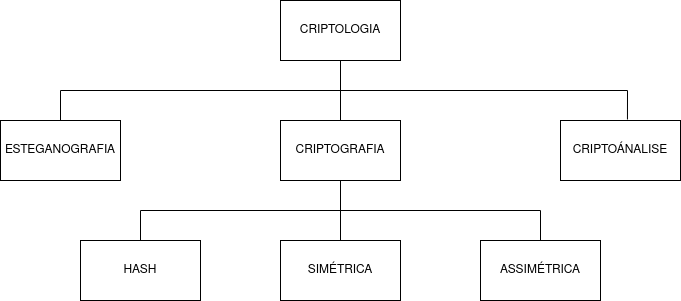
\includegraphics[width=0.75\textwidth]{Figuras/criptologia.png}\\
        \footnotesize{Fonte: O autor.}
        \label{fig:criptologia}
    \end{figure}

A criptografia possui os seguintes objetivos: confidencialidade, integridade, autenticação e irretratabilidade \cite{introduction_to_cryptography}. A confidencialidade visa garantir que um determinado dado possa ser lido apenas por destinatários autorizados. Integridade procura assegurar que um dado não seja modificado durante a transmissão. A autenticação determina que um destinatário possa verificar a origem da mensagem. Por fim, a irretratabilidade certifica que um emissor não possa negar a autoria de uma mensagem. Por si só, um algoritmo de criptografia não assegura estes objetivos e outras necessidades de segurança. Dependendo do cenário, é necessário utilizar diversos algoritmos em conjunto, cada um resolvendo uma parcela do problema. Por exemplo, ao enviar uma mensagem utilizando o \ac{ML-KEM}, iremos garantir apenas confidencialidade e integridade. Para garantir a autenticação e irretratabilidade devemos utilizar um algoritmo de assinatura digital.

Historicamente a criptografia é dividida em dois períodos: criptografia clássica e moderna. Alguns autores como \cite{criptografia_e_seguranca_de_redes,introduction_to_modern_cryptography} consideram a criptografia clássica os métodos de criptografia que antecedem a criação da criptografia assimétrica em 1976 por Whitfield Diffie e Martin Hellman, isto é, métodos de transposição, substituição, \textit{one-time pad}, máquinas de rotor, etc. A Figura \ref{fig:timeline} apresenta alguns dos sistemas de criptografia clássicos e modernos. Entre os anos de 1970 e 1980, a criptografia teve um significativo avanço com a convergência da matemática e computação na área \cite{introduction_to_modern_cryptography}, se destacando a publicação do DES \cite{des} e troca de chaves Diffie-Hellman \cite{diffie-hellman}. A partir desse período, subdisciplinas da matemática, como álgebra abstrata, teoria dos números e matemática finita; e da computação, como teoria da informação e complexidade computacional, passaram a estar presentes na criação e na utilização dos processos de criptografia, assim dando início à criptografia moderna.

    \begin{figure}[htb!]
        \centering
        \caption{Linha do tempo da criptografia.}
        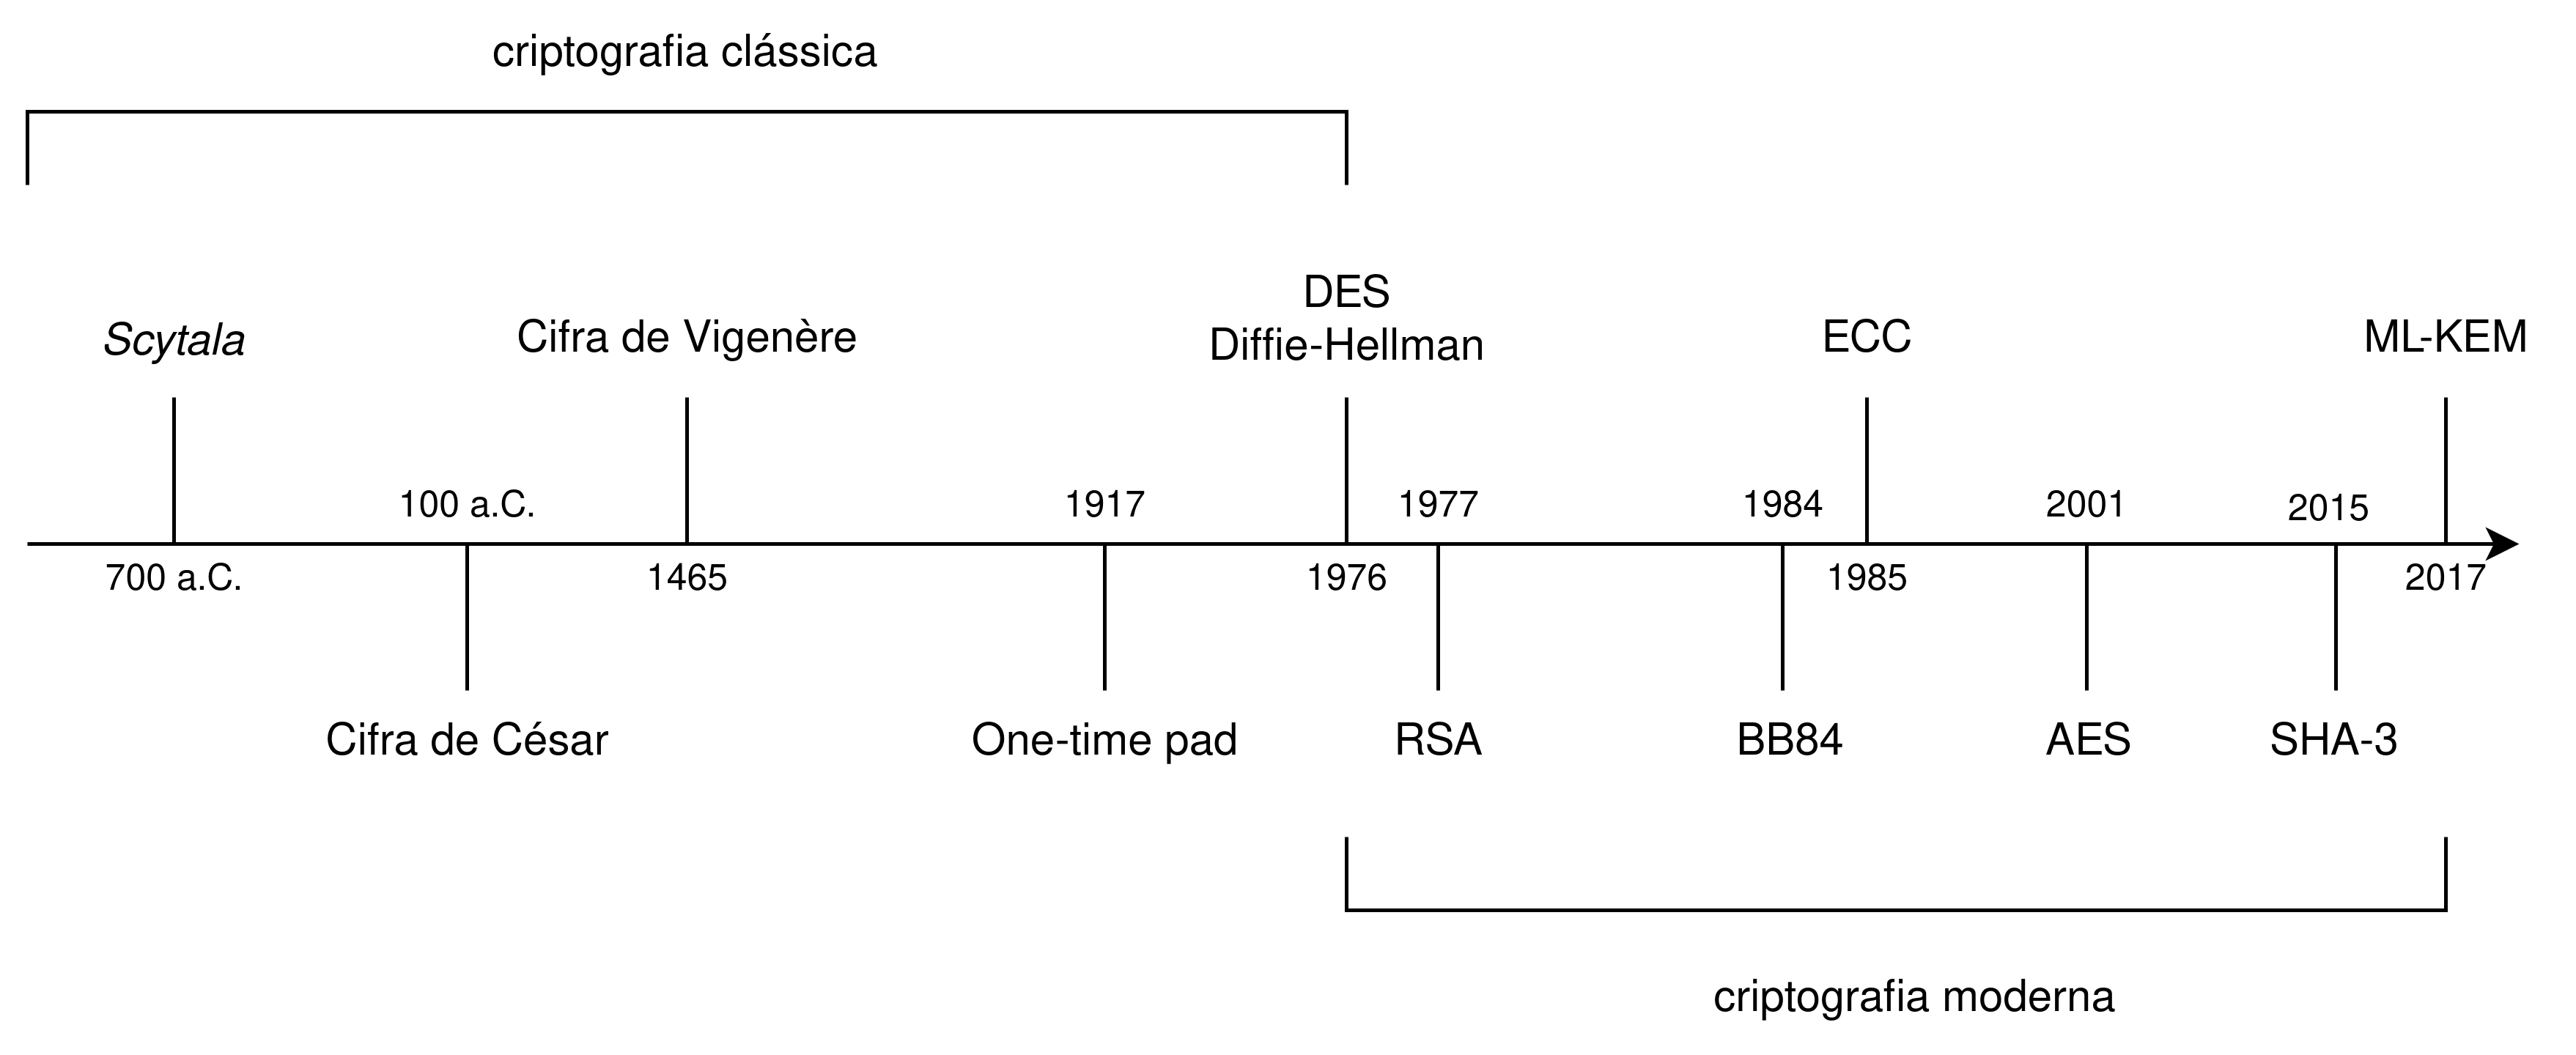
\includegraphics[width=1\textwidth]{Figuras/timeline.png}\\
        \footnotesize{Fonte: O autor.}
        \label{fig:timeline}
    \end{figure}

É importante destacar a diferença entre criptografia quântica e pós-quântica, embora os termos sejam semelhantes e podem causar uma certa confusão, eles se diferem em seu propósito e na natureza de como realizam os processos de criptografia. Os algoritmos quânticos como o BB84, desenvolvido por Charles Bennett e Gilles Brassard \cite{bb84}, utilizam as propriedades da mecânica quântica como método de criptografia. Ou seja, tem como objetivo serem executados em computadores quânticos para garantirem a segurança dos dados. A criptografia pós-quântica é um termo que surgiu devido a preocupação com a segurança das informações criptografadas com algoritmos baseados em problemas que podem ser resolvidos pelo algoritmo de Shor \cite{shor}. Estes algoritmos de criptografia pós-quânticos tem como objetivo serem executados em computadores convencionais, e serem seguros tanto contra ataques realizados por computadores clássicos quanto quânticos \cite{nist}, como é o caso do \ac{ML-KEM}.

A criptografia possui três subáreas principais, as funções \textit{hash}, criptografia simétrica e assimétrica. É importante conhecer as particularidades de cada uma dessas áreas, como, seu funcionamento, s problemas e soluções que os algoritmos destas áreas resolvem. Cada uma delas possui suas vantagens e desvantagens, com isso, são aplicáveis a problemas específicos na criptografia.

\section{Função Hash}
    Uma função \textit{hash} é uma função que mapeia uma entrada de tamanho variável em uma saída de tamanho fixo, $f:\{0,1\}^{*} \rightarrow \{0,1\}^n$. Entretanto, essas funções devem possuir algumas características para serem consideradas funções \textit{hash}:

    \begin{enumerate}
        \item[(i)] saída de tamanho fixo: independente do tamanho da entrada, a saída deve sempre ter o mesmo tamanho;
        \item[(ii)] determinístico: para uma mesma entrada, deve-se sempre obter a mesma saída;
        \item[(iii)] eficiência de operação: a operação de mapeamento deve ser rápida.
    \end{enumerate}

    Funções \textit{hash} não criptográficas são comumente utilizadas onde a segurança dos dados não é uma necessidade, por exemplo, na verificação e integridade de dados, tabelas \textit{hash}, etc. Por sua vez, as funções \textit{hash} criptográficas devem possuir propriedades adicionais para terem aplicabilidade na criptografia, essas propriedades são:

    \begin{enumerate}
        \item[(i)] resistência à pré-imagem: deve ser inviável reverter o processo de \textit{hash}, ou seja, descobrir uma entrada correspondente ao \textit{hash};
        \item[(ii)] resistência à segunda pré-imagem: dado uma entrada e seu \textit{hash}, deve ser difícil achar outra entrada com mesmo \textit{hash};
        \item[(iii)] resistência à colisão: deve ser difícil encontrar duas entradas escolhidas arbitrariamente que possuam o mesmo \textit{hash}.
    \end{enumerate}

    A complexidade de se resolver o problema do item (ii) no pior caso é de $\mathcal{O}(2^n)$, isto porque seria necessário verificar todos os resultados possíveis da função \textit{hash}, até encontrar um resultado compatível com o \textit{hash} de entrada. Já a complexidade de se resolver o problema do item (iii) é de $\mathcal{O}(2^{n/2})$, uma vez que a probabilidade de se encontrar duas mensagens diferentes escolhidas aleatoriamente que produzem o mesmo \textit{hash} é maior que 50\% em $2^{n/2}$ tentativas como demonstrado em \cite{hash_n/2, criptografia_e_seguranca_de_redes}. 

    As funções \textit{hash} criptográficas que possuem as propriedades citadas acima podem ser utilizadas na área da criptografia como, por exemplo, em armazenamento de senhas. Perceba que se fosse aplicada uma função \textit{hash} não criptográfica qualquer a uma senha e armazenada em um banco de dados, a mesma poderia ser decifrada, já que seria possível reverter o processo através da não resistência à pré-imagem. Outras aplicabilidades de funções \textit{hash} são em geradores de números pseudoaleatórios e como subprocessos em outros algoritmos de criptografia.

\section{Criptografia simétrica}
    A criptografia simétrica tem como principal característica a utilização de uma mesma chave criptográfica para a realização dos processos de cifragem e decifragem. Diferente das funções \textit{hash} criptográficas, em que o processo de decifragem não deve ser possível computacionalmente, um algoritmo de criptografia simétrico é projetado para realizar a cifragem e decifragem de uma mensagem usando uma mesma chave criptográfica. Uma mensagem cifrada utilizando um algoritmo simétrico somente pode ser decifrada com a mesma chave que a cifrou. Alguns dos algoritmos de criptografia simétrica mais utilizado é o AES \cite{aes}.

    A Figura \ref{fig:simetrica} ilustra um exemplo da utilização de um algoritmo de cifragem simétrica para o envio de uma mensagem M, no qual C é o algoritmo de cifragem, D é o algoritmo de decifragem, $SK_{AB}$ é a chave simétrica compartilhada entre A e B, e X é a mensagem cifrada.

    \begin{figure}[htb!]
        \centering
        \caption{Envio de mensagem usando criptografia simétrica.}
        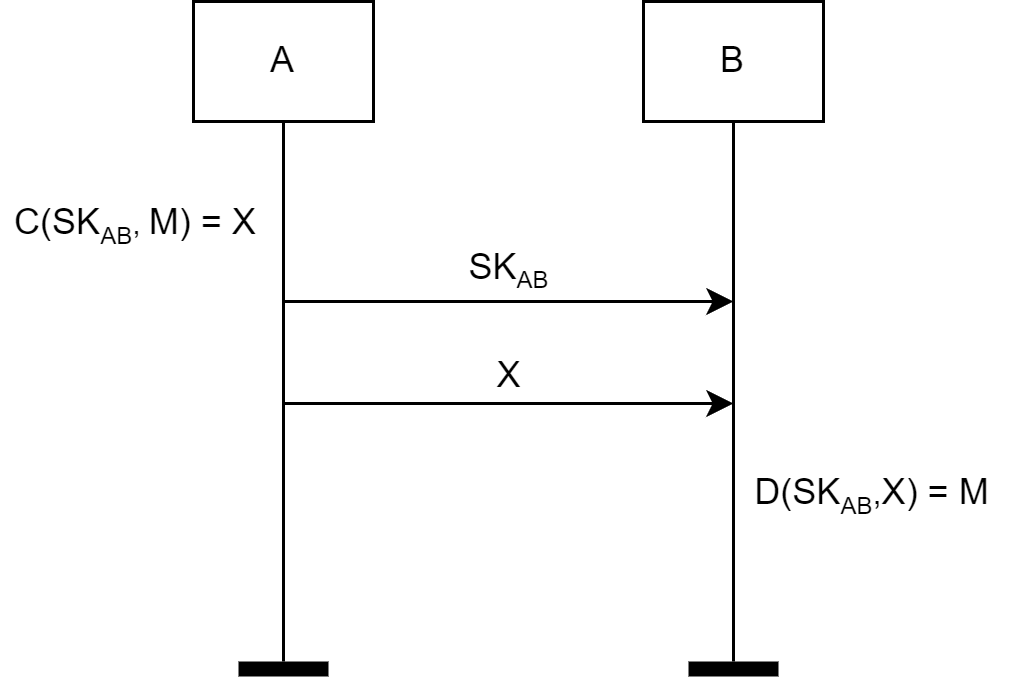
\includegraphics[width=0.65\textwidth]{Figuras/simetrica.png}\\
        \footnotesize{Fonte: O autor.}
        \label{fig:simetrica}
    \end{figure}

    Existem dois tipos de cifras simétricas quanto à forma que uma mensagem é processada: cifras de bloco e cifras em fluxo. As cifras de bloco dividem a mensagem de entrada em blocos de tamanho fixo e processam individualmente cada uma destas, para cada bloco processado se tem um bloco resultante. Caso o tamanho da mensagem não seja divisível pelo tamanho do bloco, é necessário inserir um preenchimento na mensagem de entrada. A cifra AES, por exemplo, pode operar em blocos de 128, 192 ou 256 bits. A Figura \ref{fig:cifra_bloco} ilustra uma cifra de bloco de 128 bits.

    \begin{figure}[htb!]
        \centering
        \caption{Cifra de bloco.}
        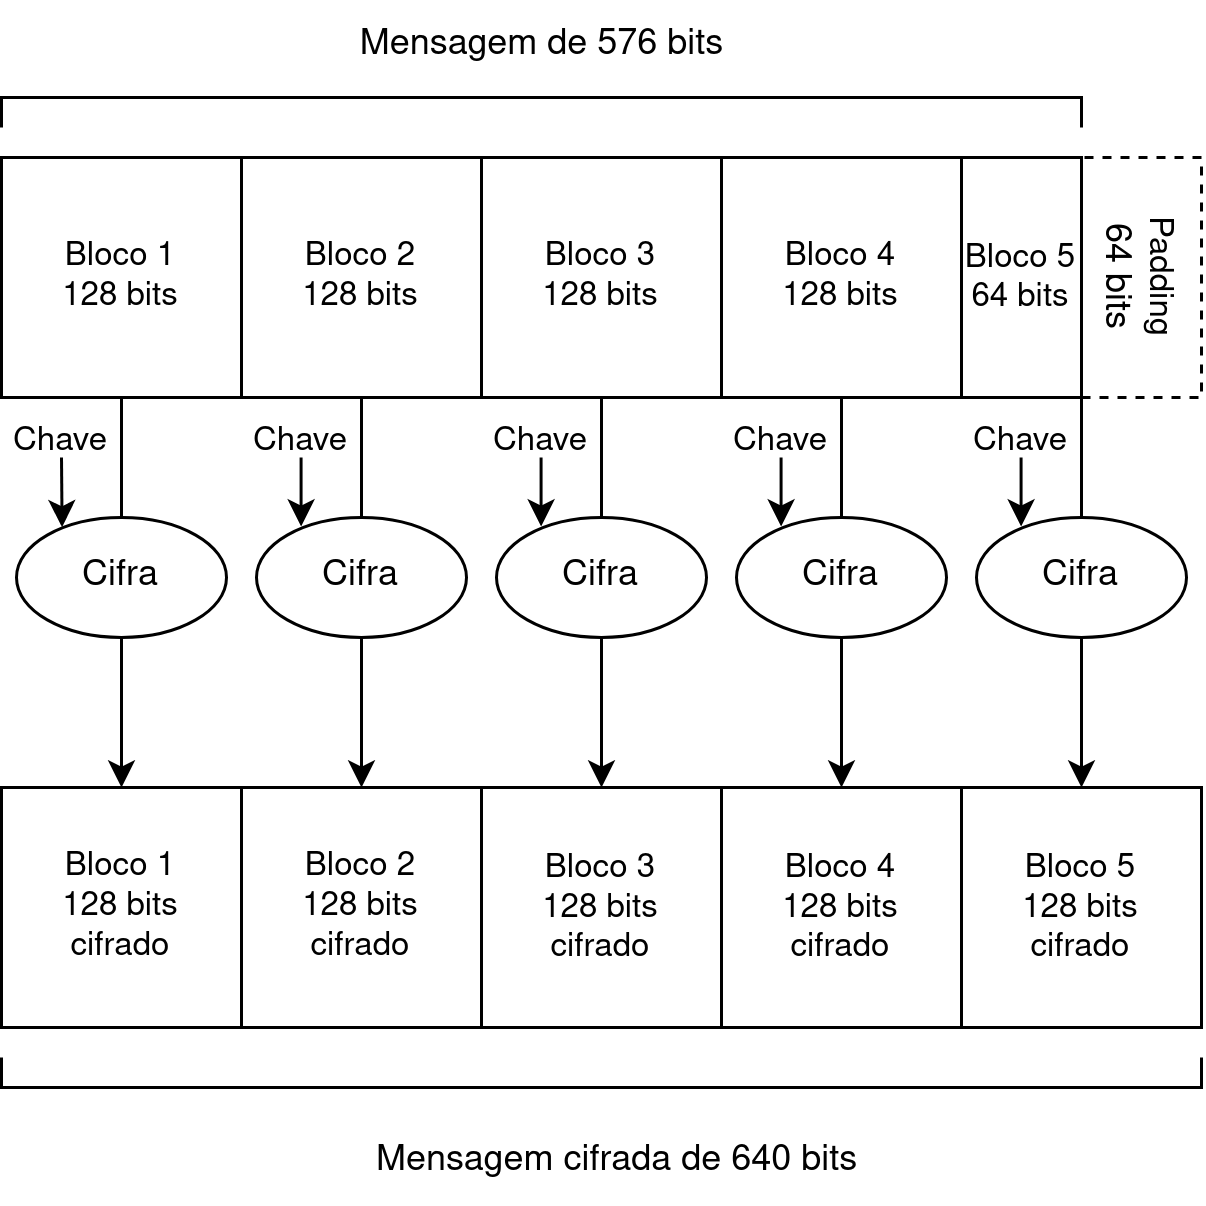
\includegraphics[width=0.65\textwidth]{Figuras/cifra_bloco.png}\\
        \footnotesize{Fonte: O autor.}
        \label{fig:cifra_bloco}
    \end{figure}
    
    As cifras em fluxo, por sua vez, processam os elementos da entrada continuamente, geralmente bit a bit, ou bytes a byte, e produzem uma saída conforme processam esses elementos. A operação $\oplus$ (XOR/ou exclusivo) é um exemplo de cifra de fluxo, na qual a cifragem consiste na aplicação da operação $\oplus$ entre um byte/mensagem e uma chave secreta de um byte,

    \begin{center}
        $\begin{array}{cll}
                   & 10010110 & \textrm{mensagem}\\
            \oplus & 01101100 & \textrm{chave secreta}\\
            \hline
                   & 11111010 & \textrm{mensagem cifrada}
        \end{array}$
    \end{center}

    \noindent
    e a decifragem é realizada simplesmente aplicado novamente a operação $\oplus$ entre o byte cifrado e a mesma chave secreta.
    
    \begin{center}
        $\begin{array}{cll}
                   & 11111010 & \textrm{mensagem cifrada}\\
            \oplus & 01101100 & \textrm{chave secreta}\\
            \hline
                   & 10010110 & \textrm{mensagem}
        \end{array}$
    \end{center}
    
    A principal limitação das cifras simétricas é que, para transmitir uma mensagem cifrada, é necessário também transmitir para a outra parte a chave que decifra esta mensagem, como pode ser visto na Figura \ref{fig:simetrica}. O fato de ter que enviar a chave por um meio de comunicação não seguro, torna necessária a utilização em conjunto com um algoritmo de cifragem assimétrica, onde este tipo de algoritmo possui a particularidade de possuir chaves diferentes para cifrar e decifrar.

    A segurança dos algoritmos de criptografia simétricos não sofreram impacto significativo pela computação quântica. Atualmente, apenas o algoritmo de Grover \cite{grover} reduz a complexidade computacional dos problemas utilizados pelos algoritmos de cifragem simétrica. Em 1996, Lov Grover publicou um algoritmo quântico capaz de realizar a busca de um valor em uma lista de $n$ elementos não ordenados com complexidade $\mathcal{O}(\sqrt{n})$, enquanto computadores clássicos conseguem realizar esta busca em $\mathcal{O}(n)$. Isto significa que um computador quântico pode encontrar uma chave simétrica de 128 bits realizando $2^{64}$ operações com o algoritmo de Grover, ao invés de $2^{128}$ por um computador clássico. Note que para manter a mesma segurança de uma chave simétrica de 128 bits, devemos alterar o tamanho da chave para 256 bits, desta forma um computador quântico terá que realizar $2^{128}$ operações, a mesma quantidade que se tinha com a computação clássica.

\section{Criptografia assimétrica}
    A criptografia assimétrica, também conhecida por criptografia de chave pública, foi inspirada pelo algoritmo de troca de chaves Diffie-Hellman em 1976. Tradicionalmente, para duas partes possuírem a mesma chave simétrica, era necessário que uma delas enviasse sua chave para a outra parte, entretanto, na maioria dos sistemas, não se tem a garantia de um canal de comunicação seguro para essa troca. O algoritmo de Diffie-Hellman \cite{diffie-hellman} foi proposto como uma solução para este problema, estabelecendo uma chave simétrica compartilhada entre duas partes sem a necessidade do envio desta por um meio de comunicação não seguro. O algoritmo de Diffie-Hellman, diferente dos algoritmos simétricos, utiliza dados privados que não devem ser compartilhados, e dados públicos que podem ser compartilhados. No final do processo, ambas as partes possuem uma informação em comum (chave simétrica), que é muito custosa de ser obtida computacionalmente a partir das informações públicas transmitidas pelo meio de comunicação. 
    
    Em 1977, Ron Rivest, Adi Shamir e Leonard Adleman publicaram o primeiro algoritmo de criptografia assimétrica, chamado RSA \cite{rsa}. Diferente do algoritmo de troca de chaves Diffie-Hellman, o RSA realiza a cifragem de mensagens, e não apenas o estabelecimento de uma chave simétrica em comum. Em um algoritmo de criptografia assimétrica como o RSA, a cifragem de uma mensagem somente pode ser realizada por uma chave pública, e a decifragem apenas pela chave privada. Desse modo, o envio de mensagens por um canal de comunicação pode ser realizado de forma segura, já que a chave privada não necessita ser transmitida para outra parte. A Figura \ref{fig:assimetrica} exemplifica esse processo, supondo que A tenha gerado suas chaves públicas e privadas previamente, A envia sua chave pública para B, que por sua vez cifra uma mensagem usando a chave pública de A e envia para A esta mensagem cifrada, A decifra a mensagem com sua chave privada. Assim como o algoritmo Diffie-Hellman, é custoso obter computacionalmente os dados privados a partir dos dados públicos nos algoritmos de criptografia assimétricos.

    \begin{figure}[htb!]
        \centering
        \caption{Envio de mensagem usando criptografia assimétrica.}
        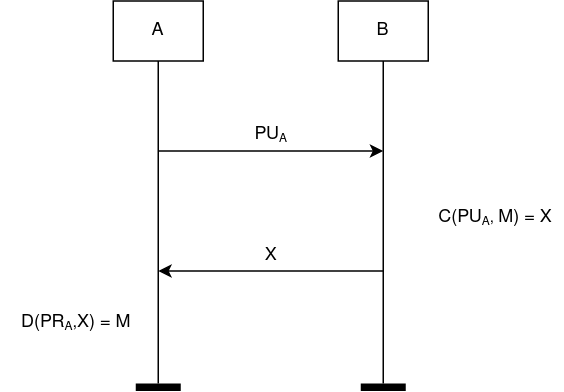
\includegraphics[width=0.65\textwidth]{Figuras/assimetrica.png}\\
        \footnotesize{Fonte: O autor.}
        \label{fig:assimetrica}
    \end{figure}

\section{Encapsulamento de chave}
\label{sec:kem}
    %é mais seguro (CCA2, PKE vs KEM)
    %pegar fontes
    %REFAZER ESTA BOSTA
    %https://www.crypto-textbook.com/download/Understanding-Cryptography-Chapter6.pdf
    Os algoritmos de criptografia assimétricos são projetados para cifrar mensagens de tamanho limitado, enquanto algoritmos simétricos são projetados para cifrar mensagens de tamanho ilimitado. Desta forma, para ser possível a comunicação de longas mensagens entre duas partes utilizando cifra simétrica, é necessária que ambas as partes tenham uma chave simétrica em comum. Atualmente, é utilizado o algoritmo de Diffie-Hellman sob a estrutura algébrica de curvas elípticas \ac{ECDH} para estabelecer esta chave simétrica em comum, entretanto, este algoritmo não é considerado seguro contra computadores quânticos por se basear no problema do logaritmo discreto. Desta forma, é utilizada outra técnica para estabelecer uma chave simétrica comum entre duas partes, chamada \ac{KEM}. A principal diferença entre a troca de chaves Diffie-Hellman e \ac{KEM} é que o algoritmo de Diffie-Hellman não permite a escolha de uma chave privada previamente, esta chave em comum é gerada ao longo do processo. O \ac{KEM}, por sua vez, funciona de uma maneira diferente, uma das partes gera a chave simétrica e a cifra usando a chave pública da outra parte. Desta forma, ambas as partes possuem uma chave simétrica em comum para utilizar em um algoritmo simétrico, e este compartilhamento de chaves é estabelecido por um algoritmo de criptografia assimétrico, neste caso, o algoritmo assimétrico deve ser resistente à computação quântica, como o \ac{ML-KEM}.

    \begin{figure}[htb!]
        \centering
        \caption{Encapsulamento de uma chave privada em comum.}
        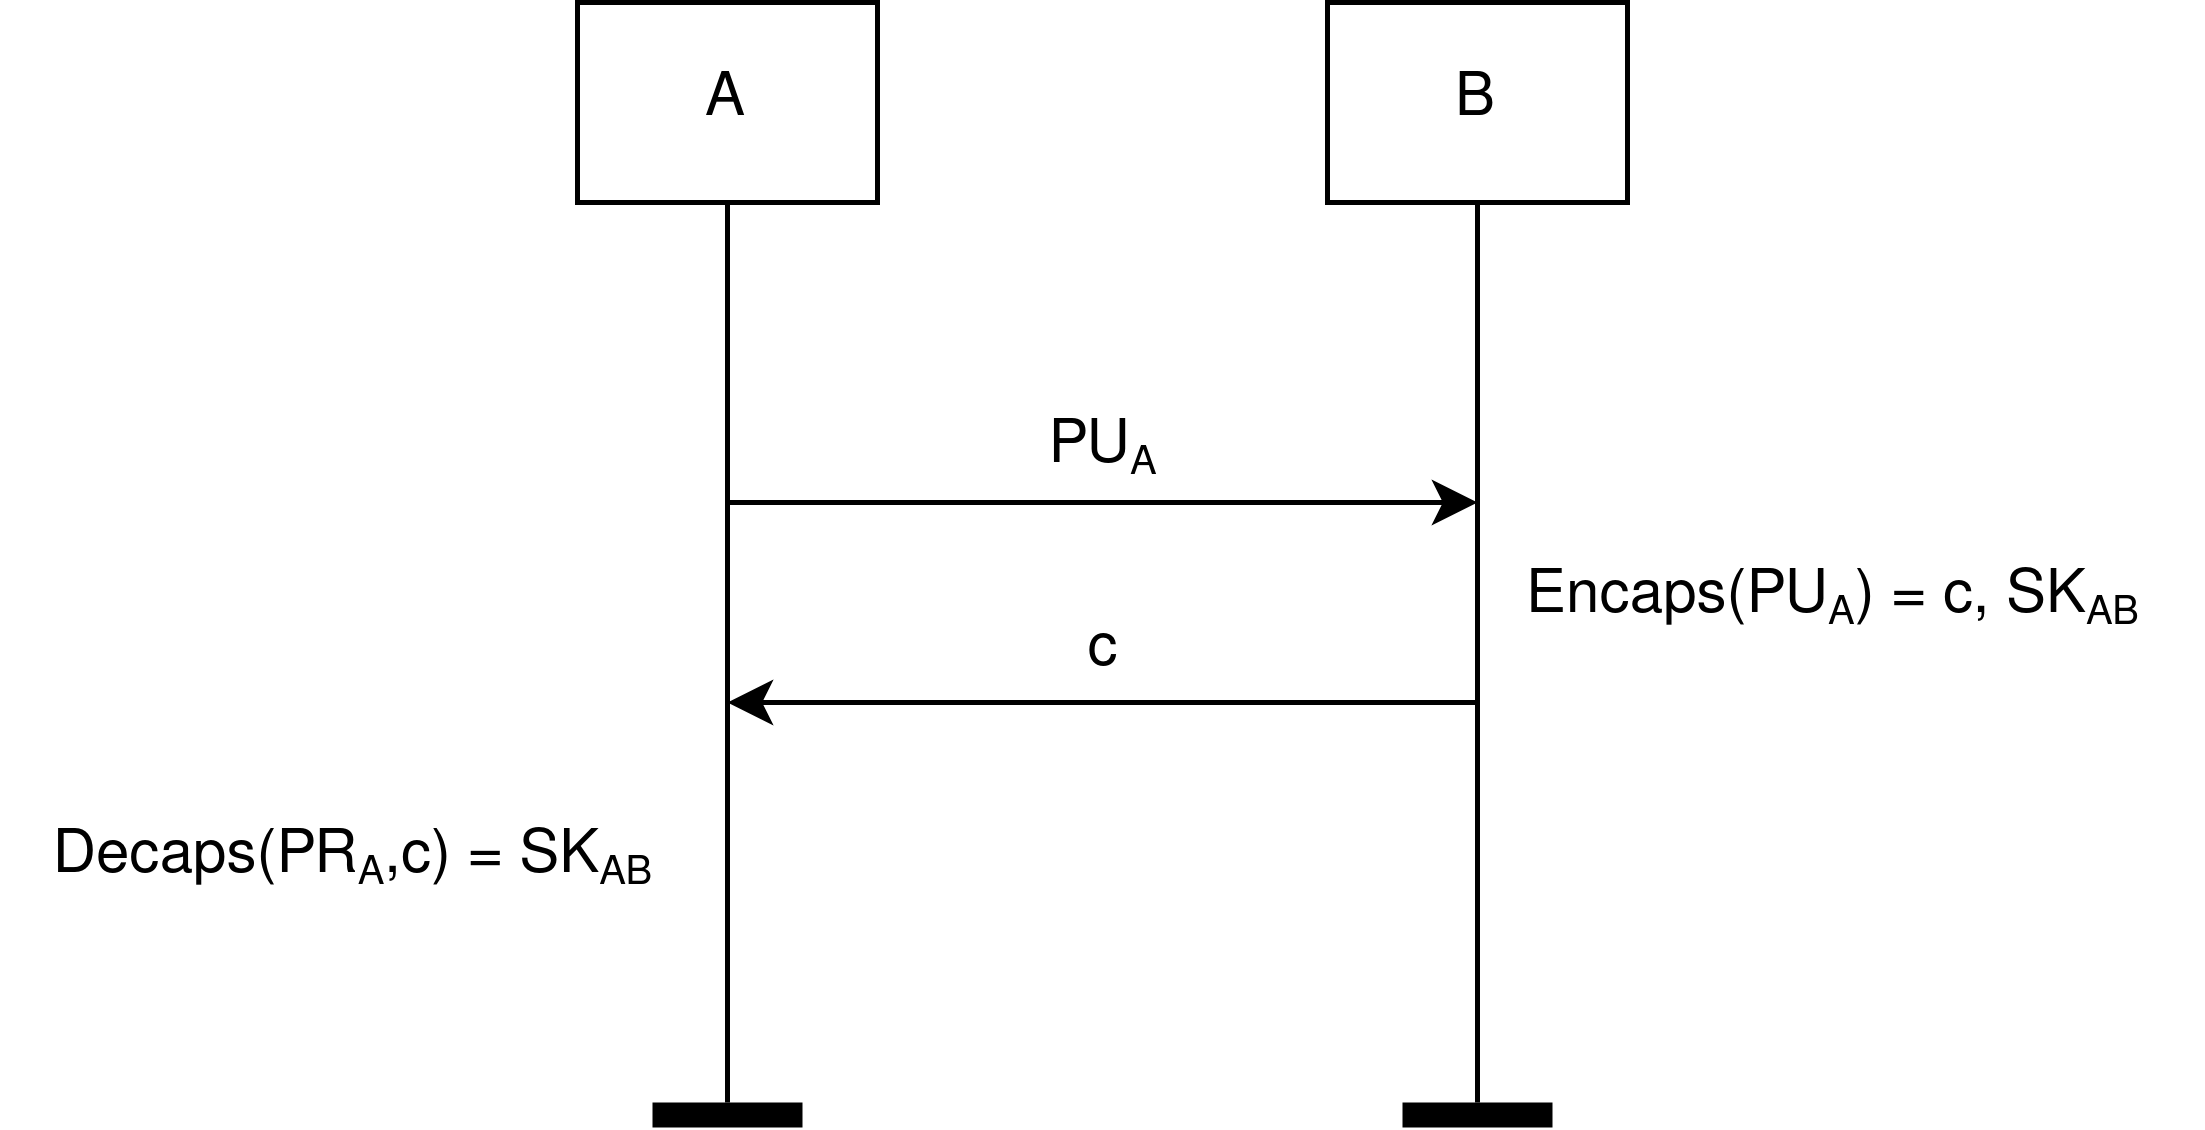
\includegraphics[width=0.75\textwidth]{Figuras/kem.png}\\
        \footnotesize{Fonte: O autor.}
        \label{fig:kem}
    \end{figure}

    O funcionamento do \ac{KEM} pode ser visto na Figura \ref{fig:kem}, na qual A envia sua chave pública $PU_A$ para B, B gera a chave simétrica comum $SK_{AB}$ e a cifra usando a chave pública de A, gerando $c$ que é enviado para A. A, por sua vez, decifra $c$ usando sua chave privada $PR_A$, gerando $SK_{AB}$. 
    
\section{Problemas computacionais}
\label{sec:problemas_computacionais}
    Alguns algoritmos de criptografia assimétrica, como Diffie-Hellman e \ac{ECDH} (Troca de chaves), RSA e \ac{ECC} (Cifragem) e RSA, \ac{ECDSA} e \ac{DSA} (Assinatura digital) possuem sua segurança baseadas nos problemas da fatoração de números inteiros e do logaritmo discreto.

    Eric Bach em \cite{discrete_logarithms_and_factoring_reductions} demonstra uma redução probabilística em tempo polinomial do problema da fatoração prima para o problema do logaritmo discreto e do problema do logaritmo discreto para o problema da fatoração prima. Isso significa que se a fatoração prima de um número $n$ for realizada, então existe uma alta probabilidade de se resolver o problema do logaritmo discreto com módulo $n$ e vice-versa. Isso implica que a complexidade de resolver ambos os problemas algoritmicamente é a mesma, se for desconsiderado o tempo da redução.
    
    A complexidade de se resolver os problemas da fatoração prima e do logaritmo discreto em um computador clássico é $\mathcal{O}(e^{(log\ n)^{1/3}(log\ (log\ n))^{2/3}})$ com o algoritmo \ac{GNFS}, considerado o algoritmo clássico mais eficiente na resolução desses problemas, enquanto o algoritmo de Shor possui a complexidade de $\mathcal{O}((log\ n)^{2}(log\ log\ n)(log\ log\ log\ n))$\cite{shor_vs_gnfs}. A Figura \ref{fig:shor_vs_gnfs} mostra um gráfico comparativo de tempo de execução entre o algoritmo de Shor e \ac{GNFS}.

    \begin{figure}[htb!]
        \centering
        \caption{Comparativo entre os algoritmos Shor e \ac{GNFS} na resolução do problema da fatoração prima de um número composto.}
        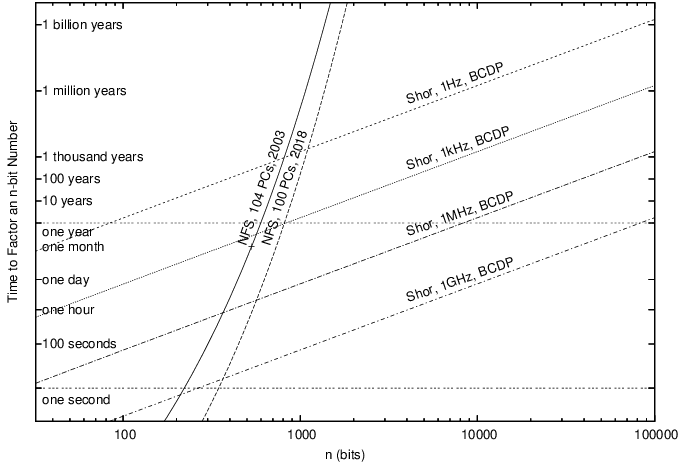
\includegraphics[width=0.75\textwidth]{Figuras/shor_vs_gnfs.png}\\
        \footnotesize{Fonte: \cite{shor_vs_gnfs}.}
        \label{fig:shor_vs_gnfs}
    \end{figure}

        \subsection{Problema da fatoração prima}
        \label{sec:problema_fatoracao_prima}
            O problema da fatoração prima de inteiros consiste em, dado um número composto, encontrar seus fatores primos. Tem-se, como exemplo, de uso de propriedades deste problema, a geração de chaves no sistema de criptografia RSA como pode ser visto no Algoritmo \ref{algo:rsa_gey_gen}. A chave pública $n$ é um número composto gerado pelo produto de dois números primos; fatorando o número $n$, descobrem-se os números primos $p$ e $q$. Obtendo os números $p$ e $q$, pode-se derivar a chave privada completa, visto que o cálculo da chave privada $d$ necessita de $e$, que é uma chave pública, e $\Phi(n)$, que é obtido através de $p$ e $q$.

            \begin{algorithm}[!htbp]
                \SetAlgoLined
                \Saida{Chave pública: $(n,e)$ e Chave privada: $(p,q,d)$}
                Escolha dois números primos $p$ e $q$\\
                Compute $n = p.q$\\
                Compute $\Phi(n) = (p - 1)(q - 1)$\\
                Escolha um expoente $e$ tal que $1 \le e < \Phi(n)$ e $mdc(e,\Phi(n))=1$\\
                Compute $d$ tal que $d.e \equiv 1\ (\textbf{mod}\ \Phi(n))$\\
                \caption{Geração de chaves RSA.}
                \label{algo:rsa_gey_gen}
            \end{algorithm}

            Este é um exemplo de como a existência de um algoritmo que fatora um número composto em tempo polinomial afeta a segurança de um dos principais algoritmos de chave pública utilizados.

        \subsection{Problema do logaritmo discreto}
        \label{sec:problema_logaritmo_discreto}
        
            O problema do logaritmo discreto consiste em, dado um número primo $p$, sua raiz primitiva $r$ e um número $n$ tal que $0 \le n < p$, encontrar o expoente $x$ que satisfaça a equação modular $n \equiv r^x\ (\textbf{mod}\ p)$. Os possíveis valores que satisfazem a equação $n \equiv r^x\ (\textbf{mod}\ p)$ compõem o conjunto finito $\mathbb{Z}_p = \{0,1,2,...,p-1\}$, e a utilização de uma raiz primitiva de $p$ como base faz com que os possíveis resultados sejam uniformemente distribuídos, isto é, de igual probabilidade de serem gerados. Isso faz com que, para encontrarmos o expoente que satisfaça a equação $n \equiv r^x\ (\textbf{mod}\ p)$, seja necessário se verificar todos os possíveis valores de $x$.

            Supondo que um emissor deseja realizar troca de chaves usando o algoritmo de Diffie-Hellmann indicado pelo Algoritmo \ref{algo:diffie-hellman}, resolvendo as equações $A \equiv g^a\ (\textbf{mod}\ p)$ e $B \equiv g^b\ (\textbf{mod}\ p)$ é possível derivar a chave secreta $s$.

            \begin{algorithm}[!htbp]
                \SetAlgoLined
                \Saida{Chave pública: $(p,g,A,B)$, Chave privada lado A: $(a,s)$, Chave privada lado B: $(b,s)$}
                O lado A e B entram em acordo publicamente para utilizar os números primos $p$ e $g$ co-primos, tal que $p > g$.\\
                O lado A escolhe um número $a$ e computa $A = g^a\ \textbf{mod}\ p$\\
                O lado B escolhe um número $b$ e computa $B = g^b\ \textbf{mod}\ p$\\
                Ambos os lados trocam entre si os valores A e B\\
                O lado A computa $s = B^a\ \textbf{mod}\ p$\\
                O lado B computa $s = A^b\ \textbf{mod}\ p$\\
                \caption{Troca de chaves Diffie-Hellman.}
                \label{algo:diffie-hellman}
            \end{algorithm}

            Este é outro exemplo de como um algoritmo que resolve o problema do logaritmo discreto pode afetar um algoritmo de criptografia que baseia sua segurança na dificuldade de se resolver o problema do logaritmo discreto.

\section{Criptoanálise}
    Quando um algoritmo de criptografia é projetado, é necessário um estudo deste algoritmo antes de ser implementado em cenários reais, para que se tenha confiança de sua segurança quando aplicado em dados sensíveis. A subárea da criptologia que visa estudar a segurança de algoritmos de criptografia é a criptoanálise. Devido à variedade de técnicas utilizadas e tipos de criptoanálise, esta seção será restrita apenas a princípios e conceitos básicos desta área, deixando as técnicas de criptoanálise referentes aos algoritmos relacionados a reticulados e ao \ac{ML-KEM} em suas respectivas seções.

    O criptógrafo holandês Auguste Kerckhoffs propôs seis princípios que deveriam ser levados em consideração ao se projetar um criptossistema militar para que este possa ser considerado seguro \cite{kerckhoffs}, são esses princípios:

    \begin{enumerate}
        \item O sistema deve ser materialmente, se não matematicamente, indecifrável;
        \item É necessário que o sistema em si não requeira sigilo, e que não seja um problema se ele cair nas mãos do inimigo;
        \item Deve ser possível comunicar e lembrar da chave sem a necessidade de notas escritas, e os interlocutores devem ser capazes de modificá-la a seu critério;
        \item Deve ser aplicável à correspondência telegráfica;
        \item O sistema deve ser portátil, e não deve exigir a participação de múltiplas pessoas na sua operação e manuseio;
        \item Por fim, o sistema deverá ser simples de usar e não exigir conhecimentos profundos ou concentração dos seus usuários nem um conjunto complexo de regras.
    \end{enumerate}

    Embora esses princípios foram criados para a tecnologia militar da época, eles ainda são válidos para os dias atuais com algumas modificações. Por exemplo, ao invés de dever ser aplicável à correspondência telegráfica, o criptossistema deve ser aplicável aos protocolos de comunicações atuais. O segundo item vai em oposição à segurança por obscuridade, cujo princípio é ocultar todo o funcionamento de um algoritmo, fornecendo o mínimo possível de informações sobre seu funcionamento; dessa forma, acredita-se que quanto menos informações for divulgada sobre o algoritmo de criptografia, mais seguro ele estará. Steven Bellovin e Randy Bush em \cite{obscurity}, argumentam que algoritmos de criptografia que utilizam a obscuridade como técnica para garantir sua segurança podem ser considerados seguros a curto prazo, mas a longo prazo somente os algoritmos publicamente analisados podem ser considerados seguros. Segundo eles, ao se ocultar as vulnerabilidades de um algoritmo de criptografia, as probabilidades de que estas possam ser reparadas diminuem, e aumentam as probabilidades de que estas vulnerabilidades possam ser exploradas por um atacante mal-intencionado. Tornar público o funcionamento de um algoritmo de criptografia permite a análise deste algoritmo pela comunidade científica, assim expondo possíveis vulnerabilidades não descobertas, tornando os algoritmos de criptografia mais seguros e confiáveis. 

    Claude Shannon em \cite{shannon} recomendou que um criptossistema deve possuir duas propriedades, confusão e difusão. O conceito de confusão em uma cifra significa que cada bit do texto cifrado deve depender de uma série de bits da chave criptográfica, dessa forma obscurecendo a relação entre a chave e o texto cifrado, o que dificulta recuperar informações da chave privada a partir do texto cifrado. A propriedade de difusão diz que, se alterado um único bit do texto original, o texto cifrado deve ser alterado em 50\% ou mais, e essas alterações devem estar esparsas no texto cifrado. A ausência desta propriedade significaria que cada bit do texto original estaria relacionado unicamente com um bit do texto cifrado, facilitando um ataque por criptoanálise.
    
    A Tabela \ref{tab:attack_model} mostra alguns modelos de ataques a esquemas de criptografia com base nas informações disponíveis ao criptoanalista, para todos os casos é considerado que o atacante possui conhecimento do algoritmo de cifragem seguindo os princípios de Kerckhoffs. Esses modelos de ataques funcionam como uma espécie de jogo, em que são fornecidas informações ao atacante e, com base nessas informações, o atacante deve ser capaz de recuperar alguma informação útil do texto cifrado. 

    \begin{table}[!htbp]
        \caption{Tipos de ataques a mensagens criptografadas.}
        \centering
        \footnotesize
        \resizebox{\textwidth}{!}{
            \begin{tabular}[h]{|p{5cm}|p{10cm}|}
                \hline
                 Tipo de ataque                & Conhecimento ao criptoanalista \\ \hline
                 Apenas texto cifrado (COA)    & Texto cifrado(desafio)  \\ \hline
                 Texto claro conhecido (KPA)   & Texto cifrado(desafio) e uma ou mais pares de texto claro e texto cifrado por uma chave secreta \\ \hline
                 Texto claro escolhido (CPA)   & Texto cifrado(desafio) e texto claro escolhido juntamente com o texto correspondente cifrado por uma chave secreta  \\ \hline
                 Texto cifrado escolhido (CCA) & Texto cifrado(desafio) e textos cifrados escolhidos juntamente com os textos correspondentes decifrados por uma chave secreta  \\ \hline
                 Texto cifrado escolhido adaptativamente (CCA2) & Texto cifrado(desafio) e textos cifrados escolhidos adaptativamente juntamente com os textos correspondentes decifrados por uma chave secreta  \\ \hline
                 Texto escolhido               & Texto cifrado, texto claro escolhido juntamente com o texto correspondente cifrado por uma chave secreta e texto cifrado pretendido, juntamente com seu texto claro correspondente decifrado por uma chave secreta \\ \hline
            \end{tabular}
        }
        \footnotesize{Fonte: Adaptado de \cite{criptografia_e_seguranca_de_redes}.}
        \label{tab:attack_model}
    \end{table}

    Os modelos de ataques são uma classificação muito utilizada para medir o nível de segurança de esquemas de criptografia. Por exemplo, se foi realizado um ataque malsucedido a um algoritmo de criptografia fornecendo apenas o texto cifrado ao atacante (COA), este algoritmo é considerado menos seguro comparado a outro algoritmo de criptografia que se teve um ataque malsucedido mesmo fornecendo mais informações como pares de textos originais e cifrados (KPA). Note que ambos os algoritmos passaram no teste de criptoanálise, entretanto o segundo algoritmo passou por uma análise mais rígida. 
    
    Outra classificação para esquemas de criptografia é a indistinguibilidade de textos cifrados, essa propriedade garante que, fornecidos pares de textos cifrados e decifrados, o atacante não deve conseguir identificar qual dos textos cifrados corresponde aos textos decifrados com probabilidade maior que 50\% \cite{introduction_to_modern_cryptography}. As três formas de indistinguibilidade de textos cifrados mais usadas na criptografia são:

    \begin{itemize}
        \item \textbf{\textit{Indistinguishability under chosen plaintext attack} (IND-CPA): } O atacante envia um par de textos para um desafiador que cifra um destes textos escolhidos aleatoriamente, e envia este texto cifrado de volta para o atacante, que por sua vez deve deduzir com uma probabilidade maior que 50\% qual dos textos foi cifrado.
        \item \textbf{\textit{Indistinguishability under (non-adaptive) chosen ciphertext attack} (IND-CCA): } O atacante pode realizar cifragens e decifragens de textos escolhidos arbitrariamente por um oráculo, e envia um par de textos para um desafiador que cifra um destes textos escolhidos aleatoriamente, e envia este texto cifrado para o atacante, que por sua vez deve deduzir com uma probabilidade maior que 50\% qual dos textos foi cifrado.
        \item \textbf{\textit{Indistinguishability under adaptive chosen ciphertext attack} (IND-CCA2): } O atacante pode realizar cifragens e decifragens de textos escolhidos arbitrariamente por um oráculo, e envia um par de textos para um desafiador que cifra um destes textos escolhidos aleatoriamente, e envia este texto cifrado para o atacante, que por sua vez pode continuar cifrando e decifrando textos (exceto o texto desafio) utilizando o oráculo para deduzir com uma probabilidade maior que 50\% qual dos textos foi cifrado. 
    \end{itemize}

    No caso do \ac{ML-KEM}, a equipe \ac{CRYSTALS} e o \ac{NIST}, o classificaram como sendo IND-CCA2 seguro \cite{kyber2}, isto significa que mesmo que fornecidos um oráculo de decifragem para um atacante, e permitir que ele realize cifragens e decifragens adaptativamente, ele não ira conseguir recuperar nenhuma informação de uma mensagem cifrada.
    
    Outra classificação para um ataque de criptoanálise segundo \cite{applied_cryptography} é com base na quantidade de recursos computacionais necessários, como a quantidade de processamento, armazenamento e dados para realizar o ataque. Embora exista um método capaz de resolver um problema computacional utilizado em um sistema criptográfico, ou recuperar informações úteis, isso não significa que este ataque seja viável computacionalmente. Por exemplo, é possível descobrir uma senha cifrada por uma função \textit{hash} através de um ataque por força bruta, em que são testadas todas as combinações possíveis, entretanto analisar todas as possibilidades levaria uma quantidade de tempo muito grande. Dessa forma, mesmo que exista uma forma de recuperar a senha por força bruta, esta função \textit{hash} é considerada segura contra este ataque devido ao tempo de processamento necessário. Existem diversos métodos que quebram o \ac{ML-KEM}, mas todos eles demandam muitos recursos computacionais para recuperar alguma informação útil do texto original \cite{kyber2}.

\section{Considerações finais}
    Este capítulo tem a finalidade de fornecer informações essenciais sobre criptografia para que o leitor possa entender o funcionamento do algoritmo \ac{ML-KEM} e assuntos relacionados. São apresentados os principais tipos de criptografia, os problemas da fatoração prima e do logaritmo discreto, estes empregados nos principais algoritmos de criptografia atuais e ameaçados pelo algoritmo de Shor. No Capítulo \ref{cap:reticulados}, é apresentada a estrutura de reticulados, na qual são estabelecidos problemas matemáticos de difícil resolução até mesmo por computadores quânticos, utilizados em algoritmos de criptografia pós-quânticos baseados nesta estrutura.
\chapter{Reticulados}
\label{cap:reticulados}
%https://repositorio.unifesp.br/bitstream/handle/11600/60730/Lucas_Eduardo_Trabalho_de_Graduacao_Final.pdf?sequence=7&isAllowed=y

    Reticulados são objetos geométricos que podem ser descritos como pontos de uma grade regular n-dimensional \cite{daniele-lattices}. Esta estrutura tem sido alvo de pesquisadores da área da criptografia devido a problemas computacionais de difícil resolução tanto para computadores convencionais quanto para computadores quânticos. Tais problemas computacionais foram utilizados na construção de sistemas criptográficos como \ac{ML-KEM} \cite{kyber}, Dilithium \cite{dilithium}, NTRU \cite{ntru} e FALCON \cite{falcon}. Este capítulo é dedicado ao estudo e aplicabilidades dos reticulados na área da criptografia.

\begin{definition}[reticulado]
    Um reticulado $\mathcal{L}$ é um subgrupo aditivo discreto de $\mathbb{R}^{n}$, ou seja, satisfaz as seguintes propriedades:

    \begin{itemize}
        \item[(i)] fechado para adição: $\forall x,y \in \mathcal{L},\ x+y \in \mathcal{L}$;
        \item[(ii)] discreto: $\forall x,y \in \mathcal{L}$, em que $x \neq y$, existe um valor $\epsilon > 0$ tal que a distância entre eles é $\lVert x-y \rVert \ge \epsilon$.
    \end{itemize}
\end{definition}

    As Figuras \ref{fig:lattice-2d} e \ref{fig:lattice-3d} ilustram um exemplo de um reticulado de duas dimensões e três dimensões respectivamente.
    
    \begin{figure}[htb!]
        \begin{minipage}[c]{0.5\linewidth}
            \centering
            \caption{Reticulado de duas dimensões.}
            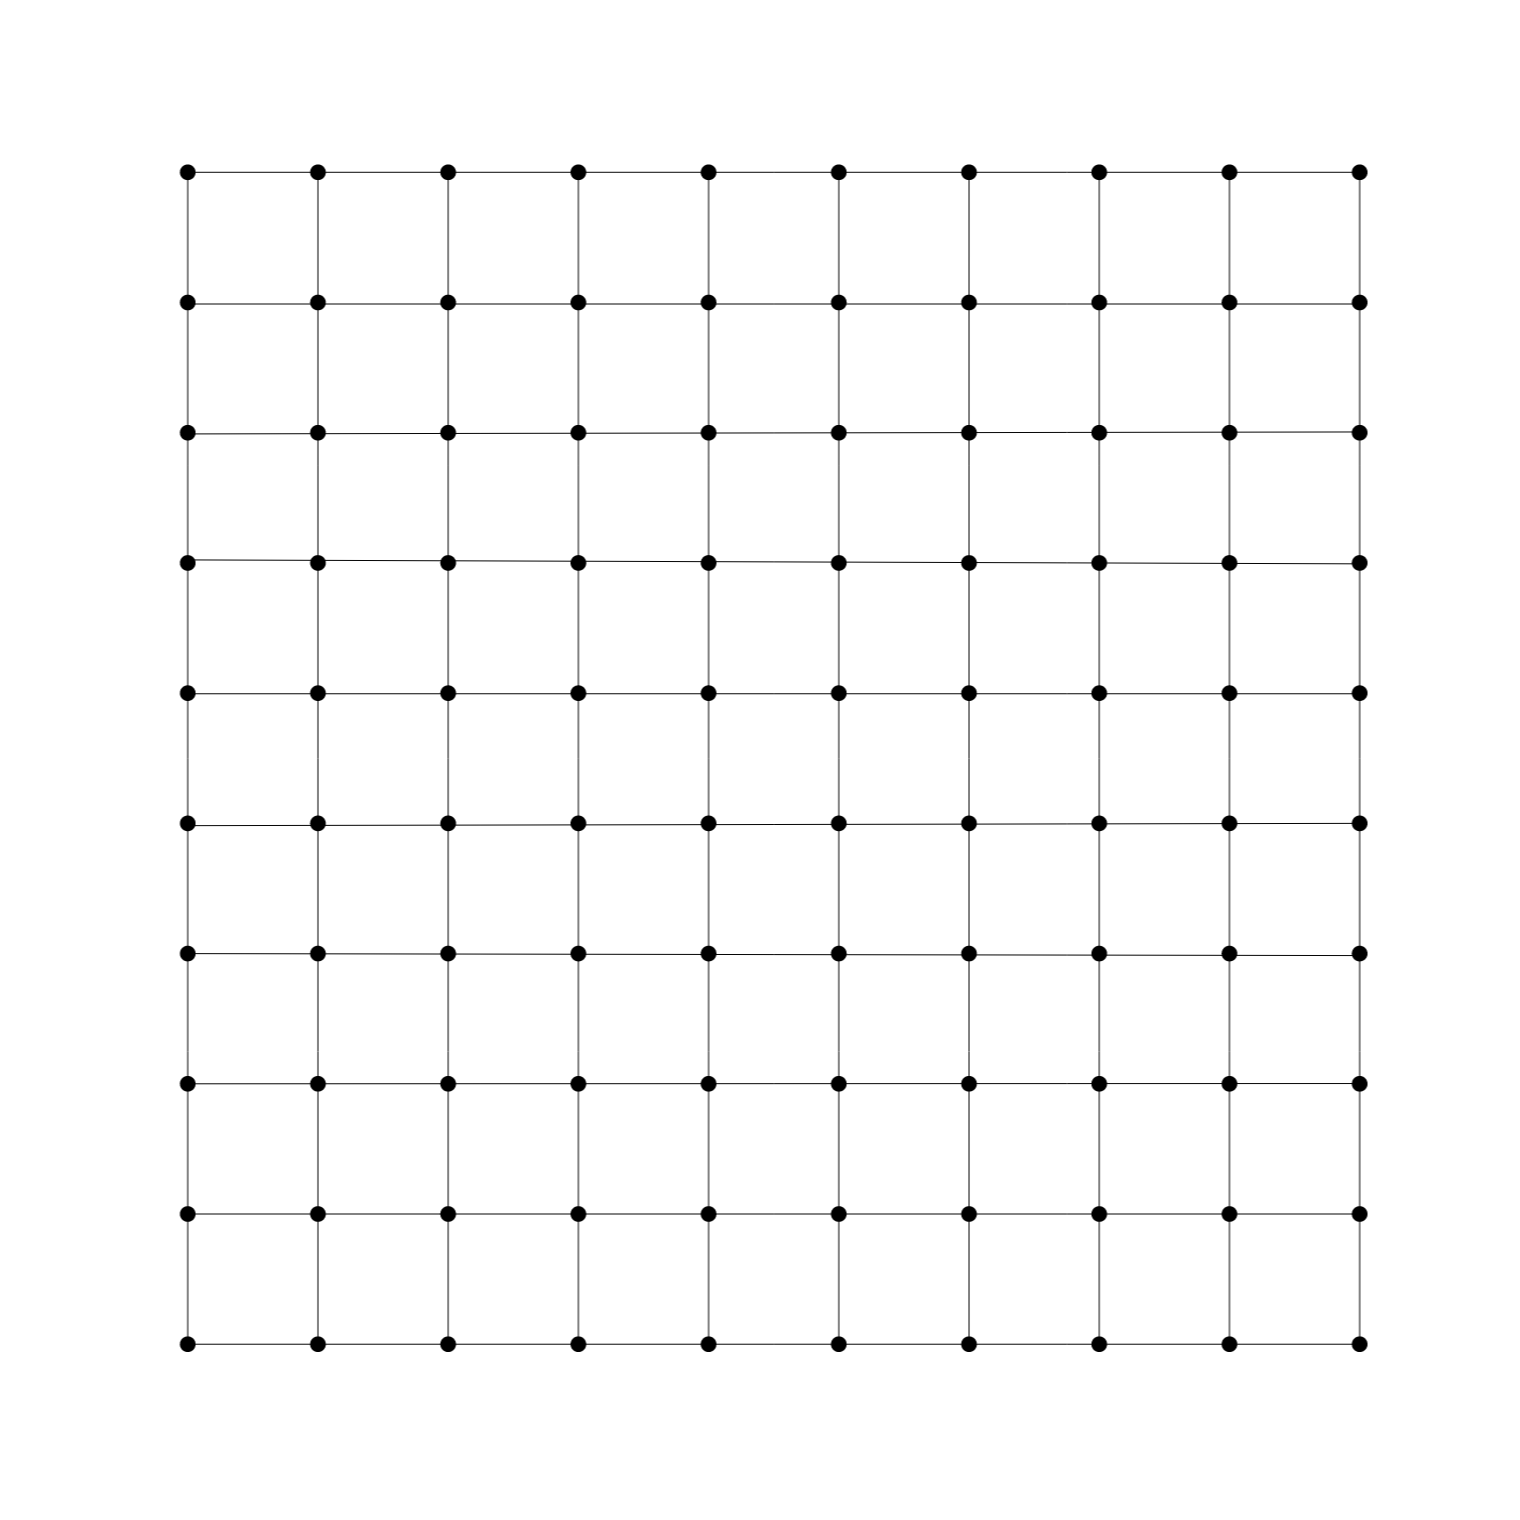
\includegraphics[width=0.75\textwidth]{Figuras/lattice-2d.png}\\
            \footnotesize{Fonte: O autor.}
            \label{fig:lattice-2d}
        \end{minipage}\hfill
        \begin{minipage}[c]{0.5\linewidth}
            \centering
            \caption{Reticulado de três dimensões.}
            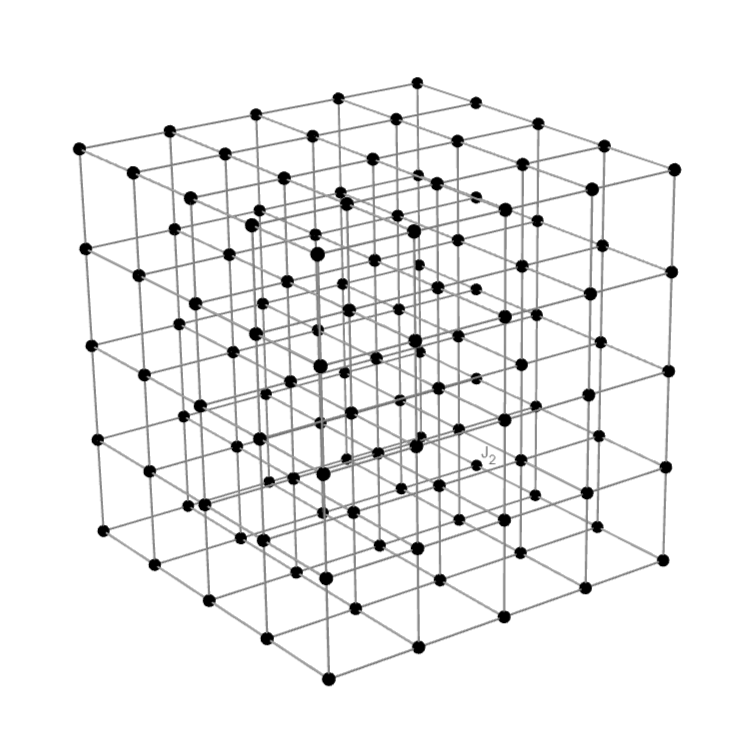
\includegraphics[width=0.75\textwidth]{Figuras/lattice-3d.png}\\
            \footnotesize{Fonte: O autor.}
            \label{fig:lattice-3d}
        \end{minipage}
    \end{figure}


\section{Base de um reticulado}
    %estou usando d para quantidade de vetores e para quantidade de componentes
    Assim como os espaços vetoriais podem ser representados/gerados por uma combinação linear entre vetores linearmente independentes, os reticulados também, com exceção que os coeficientes da combinação linear devem pertencer ao conjunto $\mathbb{Z}$, o que faz com que esta estrutura seja regular \cite{daniele-lattices}. A definição de um reticulado $\mathcal{L(\beta)}$, gerado por uma base $\beta = \{b_0, b_1, ... , b_{n-1}\} \subset \mathbb{R}^{n}$, é expressa por: 
    
    $$\mathcal{L(\beta)} = \Biggl\{\sum_{i=0}^{n-1} m_i b_i\ |\ m_i\in\mathbb{Z},\ b_i \in \beta \Biggl\},$$

    Um elemento de um reticulado, por sua definição, é representado por um vetor ou ponto. Entretanto, devido aos isomorfismos aditivos $\sigma_1$ e $\sigma_2$, é possível representar os elementos de um reticulado na forma polinomial ou matricial respectivamente. A representação de um elemento na forma polinomial possui mais utilidade em alguns problemas específicos envolvendo reticulados como \ac{RLWE} e \ac{MLWE}.
    
    $\begin{array}{rl}
        \sigma_1 &:P[x] \to \mathbb{Z}^n\\
               &:a_0 + a_1 x + a_2 x^2 + ... + a_{n-1} x^{n-1} \to (a_0, a_1, a_2, ... , a_{n-1})
    \end{array}$\\\\

    $\begin{array}{rl}
        \sigma_1^{-1} &:\mathbb{Z}^n \to P[x]\\
               &:(a_0, a_1, a_2, ... , a_{n-1}) \to a_0 + a_1 x + a_2 x^2 + ... + a_{n-1} x^{n-1}
    \end{array}$\\\\

    Através do isomorfismo $\sigma_1$ é possível transformar um polinômio na forma $a_0 + a_1 x + a_2 x^2 + ... + a_{n-1} x^{n-1}$ em um ponto ou vetor na forma $(a_0, a_1, a_2, ... , a_{n-1})$. O inverso desse isomorfismo, representado por $\sigma_1^{-1}$, realiza o mapeamento inverso, transformando um ponto em um polinômio. Por outro lado, a representação de um elemento de um reticulado na forma matricial facilita a visualização na realização dos cálculos dos principais problemas computacionais sobre esta estrutura.
    
    $\begin{array}{rl}
            \sigma_2 &:M_n \to \mathbb{Z}^n\\
                   &:[a_0\ a_1\ a_2\ ...\ a_{n-1}] \to (a_0, a_1, a_2, ... , a_{n-1})
    \end{array}$\\\\

    $\begin{array}{rl}
            \sigma_2^{-1} &:\mathbb{Z}^n \to M_n\\
                   &:(a_0, a_1, a_2, ... , a_{n-1}) \to [a_0\ a_1\ a_2\ ...\ a_{n-1}]
    \end{array}$\\\\

    O isomorfismo aditivo $\sigma_2$ e sua inversa $\sigma_2^{-1}$, por sua vez, transformam uma matriz linha ou coluna em um elemento de $\mathbb{Z}^n$ e vice-versa. Estes isomorfismos aditivos significam que um elemento de um reticulado representado por um ponto, vetor, matriz ou polinômio, possui o mesmo comportamento com relação à operação de adição.

    Uma base $\beta = \{b_0, b_1, ... b_{n-1}\} \subset \mathbb{R}^{n}$ de um reticulado também pode ser representada na forma matricial devido ao isomorfismo $\sigma_2$, na qual as componentes dos vetores da base formam as colunas da matriz geradora do reticulado. Seja $\textbf{B} = [b_0\ b_1\ ...\ b_{n-1}] \in \mathbb{R}^{d \times n}$ a base do reticulado $\mathcal{L}$ na forma matricial, $\mathcal{L}(\textbf{B})$ pode ser representada por:

    $$\mathcal{L}(\textbf{B}) = \{\textbf{B}x\ |\ x \in \mathbb{Z}^n\},$$

    \noindent
    em que $\textbf{B}x$ é uma multiplicação matricial usual, $d$ representa o número de componentes dos vetores de $\textbf{B}$ e $n$ representa a dimensão do reticulado $\mathcal{L}(\textbf{B})$. Quando o número de componentes dos vetores da base de um reticulado coincide com seu grau, ou seja, a base do reticulado na forma matricial possui posto completo\footnote{Em outras palavras: tem-se uma matriz quadrada.}, o reticulado é dito completo.

    Ambas as formas de representação de um reticulado são equivalentes, isso pode ser verificado derivando a notação por combinação linear a partir da notação matricial:

    \begin{center}
        $\begin{bmatrix}
                b_{0 0} & b_{0 1} & . & . & . & b_{0 (n-1)}\\
                b_{1 0} & b_{1 1} & . & . & . & b_{1 (n-1)}\\
                b_{2 0} & b_{2 1} & . & . & . & b_{2 (n-1)}\\
                .      & .      & . &   &   & .     \\
                .      & .      &   & . &   & .     \\
                .      & .      &   &   & . & .     \\
                b_{(d-1) 0} & b_{(d-1) 1} &   &   &   & b_{(d-1) (n-1)}
            \end{bmatrix}$
        %
        $\begin{bmatrix}
            x_0\\
            x_1\\
            x_2\\
            .  \\
            .  \\
            .  \\
            x_{n-1}
        \end{bmatrix}$
        %
        $\Leftrightarrow$\\
    \end{center}

    \begin{center}
        $x_0\begin{bmatrix} b_{00} \\ b_{01} \\ b_{02} \\ . \\ . \\ . \\ b_{0 (d-1)} \end{bmatrix}$ + 
        $x_1\begin{bmatrix} b_{10} \\ b_{11} \\ b_{12} \\ . \\ . \\ . \\ b_{1 (d-1)} \end{bmatrix}$ +
        $x_2\begin{bmatrix} b_{20} \\ b_{21} \\ b_{22} \\ . \\ . \\ . \\ b_{2 (d-1)} \end{bmatrix}$ + ... +
        $x_{n-1}\begin{bmatrix} b_{(n-1) 0} \\ b_{(n-1) 1} \\ b_{(n-1) 2} \\ . \\ . \\ . \\ b_{(n-1) (d-1)} \end{bmatrix}$
        %
        $\Leftrightarrow$\\
    \end{center}

    \begin{center}
        $x_0 \vec{b_0} + x_1 \vec{b_1} + x_2 \vec{b_2} + ... + x_{n-1} \vec{b_{n-1}}$
    \end{center}

    Existem alguns tipos de reticulados que devem ser mencionados para melhor compreensão dos conceitos utilizados posteriormente neste trabalho.

    \begin{definition}[reticulado inteiro]
        Um reticulado $\mathcal{L}(\textbf{B})$ é dito inteiro se os coeficientes dos vetores da base $\textbf{B}$ forem inteiros, ou seja, $\mathcal{L}(\textbf{B}) = \{\textbf{B}x\ |\ \textbf{B} \in \mathbb{Z}^{d \times n},\ x \in \mathbb{Z}^n\}$.
    \end{definition}

    %https://simons.berkeley.edu/sites/default/files/docs/14953/intro.pdf
    \begin{definition}[reticulado dual]
        A dual de um reticulado $\mathcal{L}$, denotado por $\mathcal{L}^{*}$, é o conjunto de todos os vetores $\vec{x} \in span(\mathcal{L})$ tal que $\langle \vec{x},\vec{y} \rangle \in \mathbb{Z}$, para todo $\vec{y} \in \mathcal{L}$.
    \end{definition}

    \begin{definition}[reticulado ideal]
    \label{ideal_lattice}
        Seja um anel $A$ e um isomorfismo aditivo $\sigma$ que mapeia $A$ para $\sigma (A) \subset \mathbb{R}^n$. Um reticulado ideal é um $\sigma(I)$ para um ideal $I \subseteq A$ \cite{ring_lwe}.
    \end{definition}

    Segundo a Definição \ref{ideal_lattice}, um reticulado ideal é obtido aplicando um isomorfismo aditivo que mapeia um ideal para um subconjunto de $\mathbb{R}^n$. A estrutura $\mathbb{Z}{[}x{]}/ \langle x^n + 1 \rangle$, na qual é abordada na Seção \ref{cap:lattice_problems} e pode ser consultada no Apêndice \ref{ap:conceitos_matematicos}, representa a um reticulado ideal, visto que existe um isomorfismo aditivo que mapeia um polinômio pertencente ao ideal $\langle x^n + 1 \rangle$ para um subconjunto de $\mathbb{R}^n$, neste caso $\mathbb{Z}^n$.

    \begin{definition}[reticulado modular]
    \label{modular_lattice}
        Seja um anel $A$ e um isomorfismo aditivo $\sigma$ que mapeia $A$ para $\sigma (A) \subset \mathbb{R}^n$. Um reticulado modular é definido por uma função que mapeia um conjunto $\{ \sigma(A)_1,\sigma(A)_2,...,\sigma(A)_d \}$ para $\mathbb{R}^{nd}$ \cite{module-lwe}. 
    \end{definition}

    Um reticulado modular é um subconjunto de um espaço vetorial gerado por um conjunto finito de vetores fechado sob operações de soma e multiplicação por escalares em um anel comutativo. Tem-se como exemplo uma matriz de ordem $n \times n$ em que os elementos desta matriz pertencem a um anel. Se houver um isomorfismo que mapeia os elementos desta matriz para um subconjunto de $\mathbb{R}^n$ e que esta matriz respeita as propriedades de módulo, então pode-se afirmar que esta matriz pertence a um módulo.

\section{Domínio fundamental}
    O domínio fundamental de um reticulado $\mathcal{L}(\textbf{B})$, denotado por $\mathcal{F}_B$, é a região do paralelepípedo de dimensão $n$ formado pelos vetores geradores de $\mathcal{L} \subset \mathbb{R}^{n}$. Tal paralelepípedo é expresso geometricamente pela fórmula abaixo: 

     $$\mathcal{F}_B = \{\textbf{B}x\ |\ 0 \le x_i < 1\},$$

     \noindent
     na qual $x_i$ são as componentes do vetor $x$, como pode ser visto na Figura \ref{fig:dominio_fundamental}. 

     \begin{figure}[htb!]
        \centering
        \caption{Ilustração de um domínio fundamental.}
        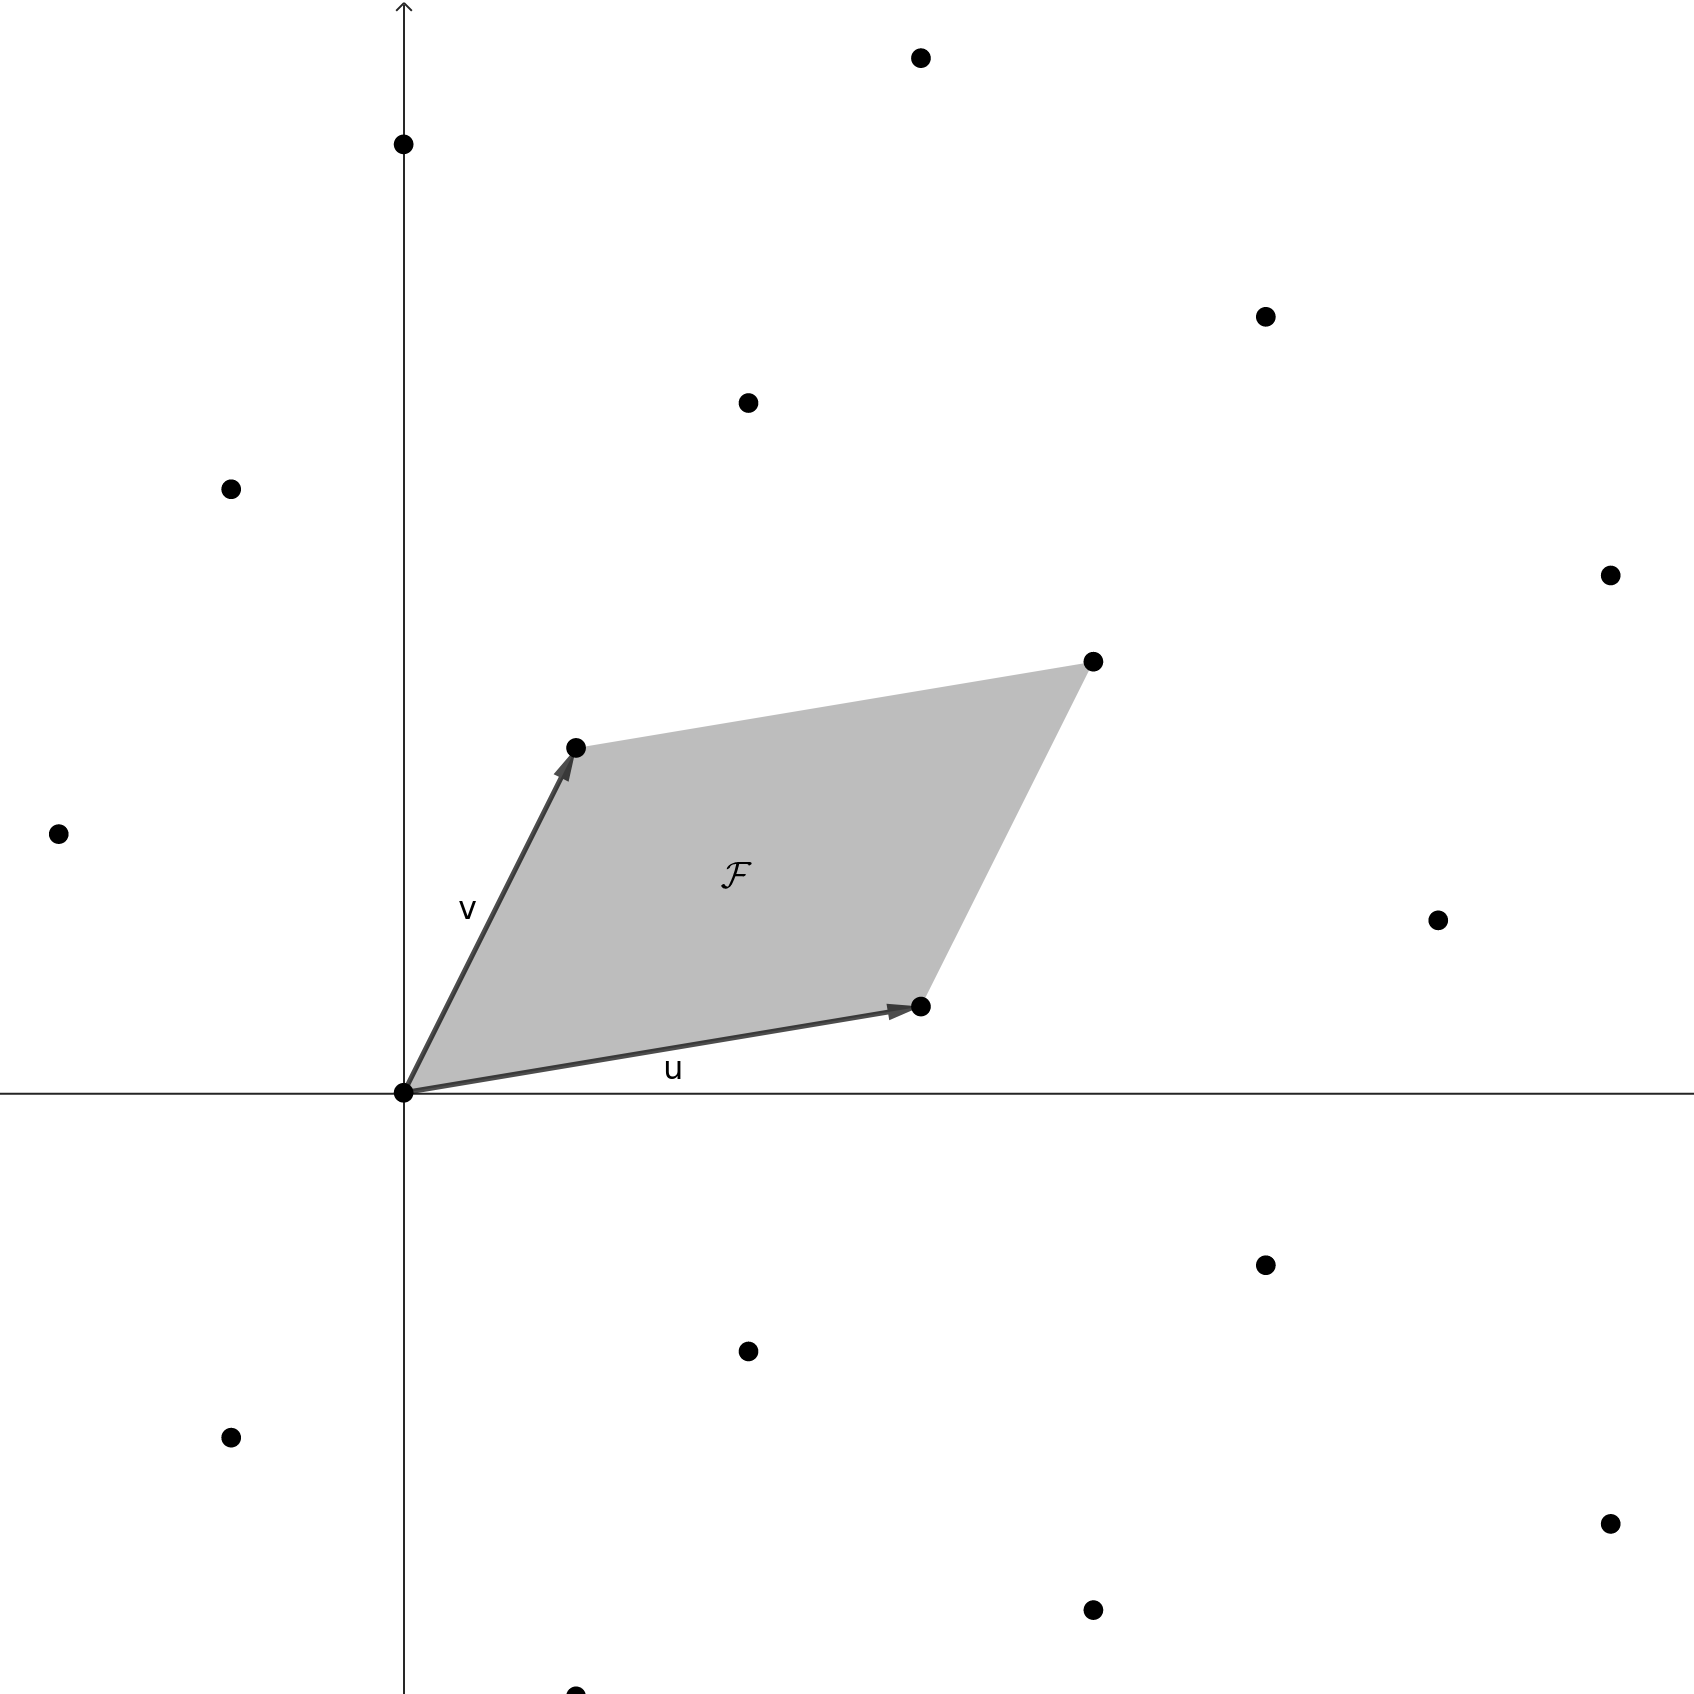
\includegraphics[width=0.75\textwidth]{Figuras/dominio_fundamental.png}\\
        \footnotesize{Fonte: O autor.}
        \label{fig:dominio_fundamental}
    \end{figure}

    As regiões sombreadas da Figura \ref{fig:dominio_fundamental_2} representam os domínios fundamentais de um mesmo reticulado de dimensão 2 gerado por duas bases diferentes, na qual as áreas dos dois paralelepípedos são as mesmas e nenhum elemento do reticulado está no domínio fundamental, com exceção da origem. Isto significa que ambas as bases geram este mesmo reticulado. Esta é uma das propriedades dos domínios fundamentais segundo \cite{daniele-lattices}.

    \begin{figure}[htb!]
        \caption{Exemplo de domínios fundamentais diferentes com mesma área.}
        \begin{minipage}[c]{0.5\linewidth}
            \centering
            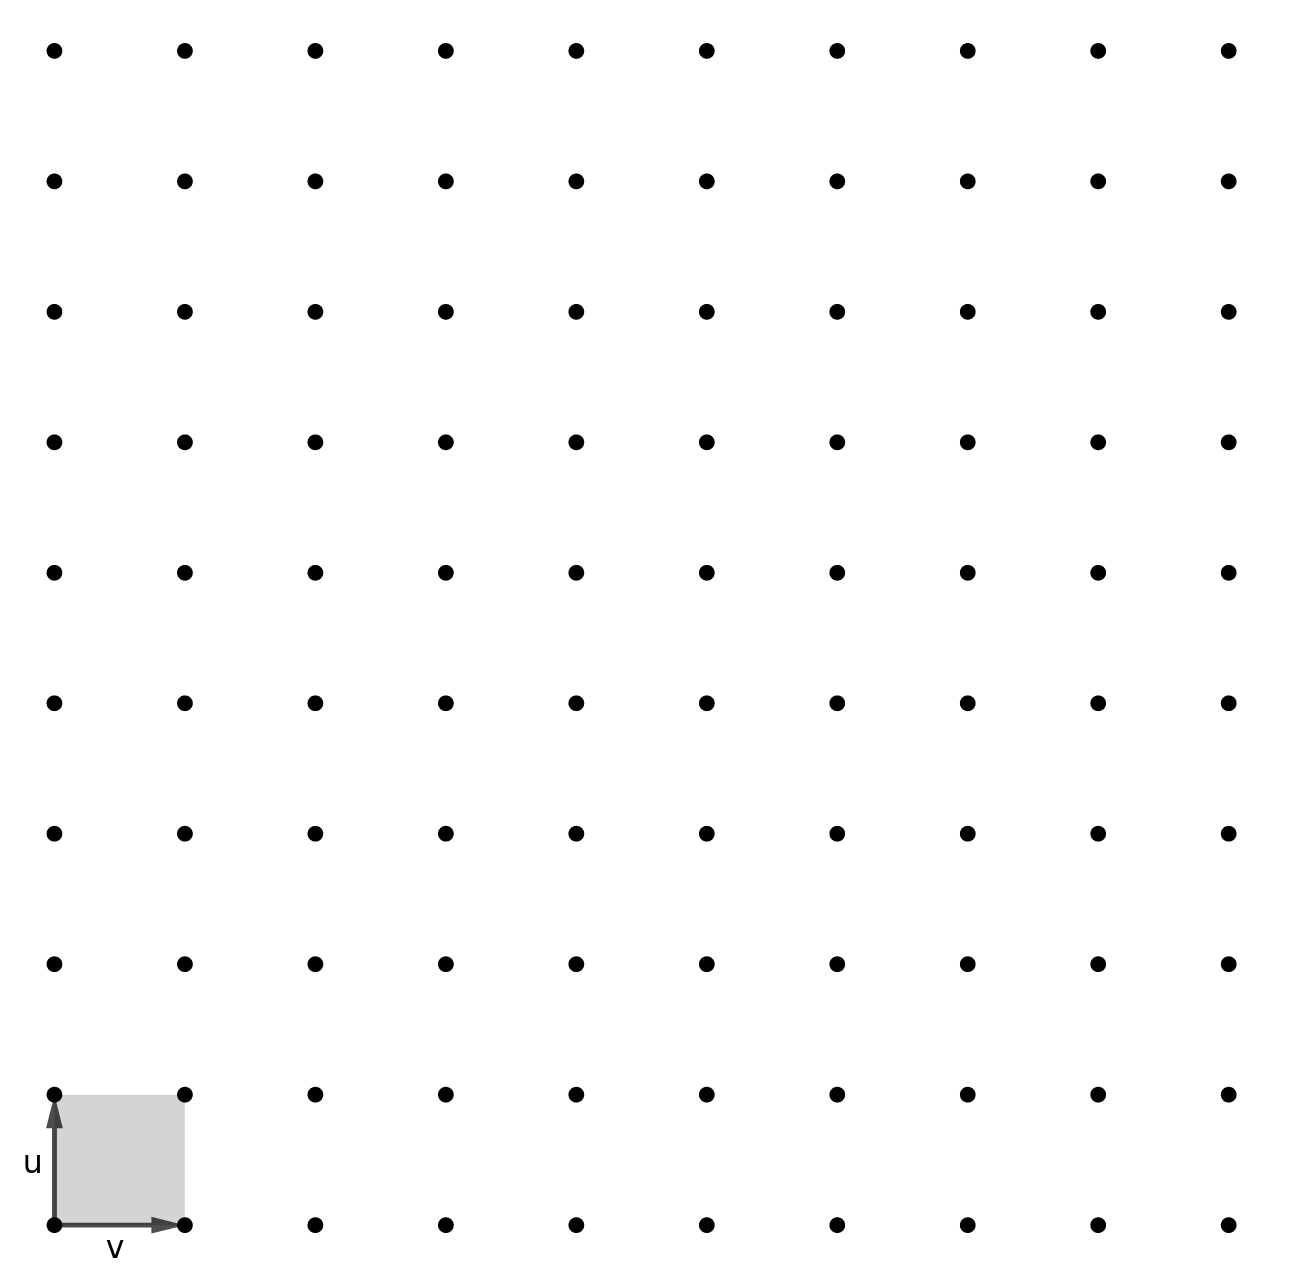
\includegraphics[width=0.75\textwidth]{Figuras/dominio_fundamental_1.png}\\
            \footnotesize{Fonte: O autor.}
        \end{minipage}\hfill
        \begin{minipage}[c]{0.5\linewidth}
            \centering
            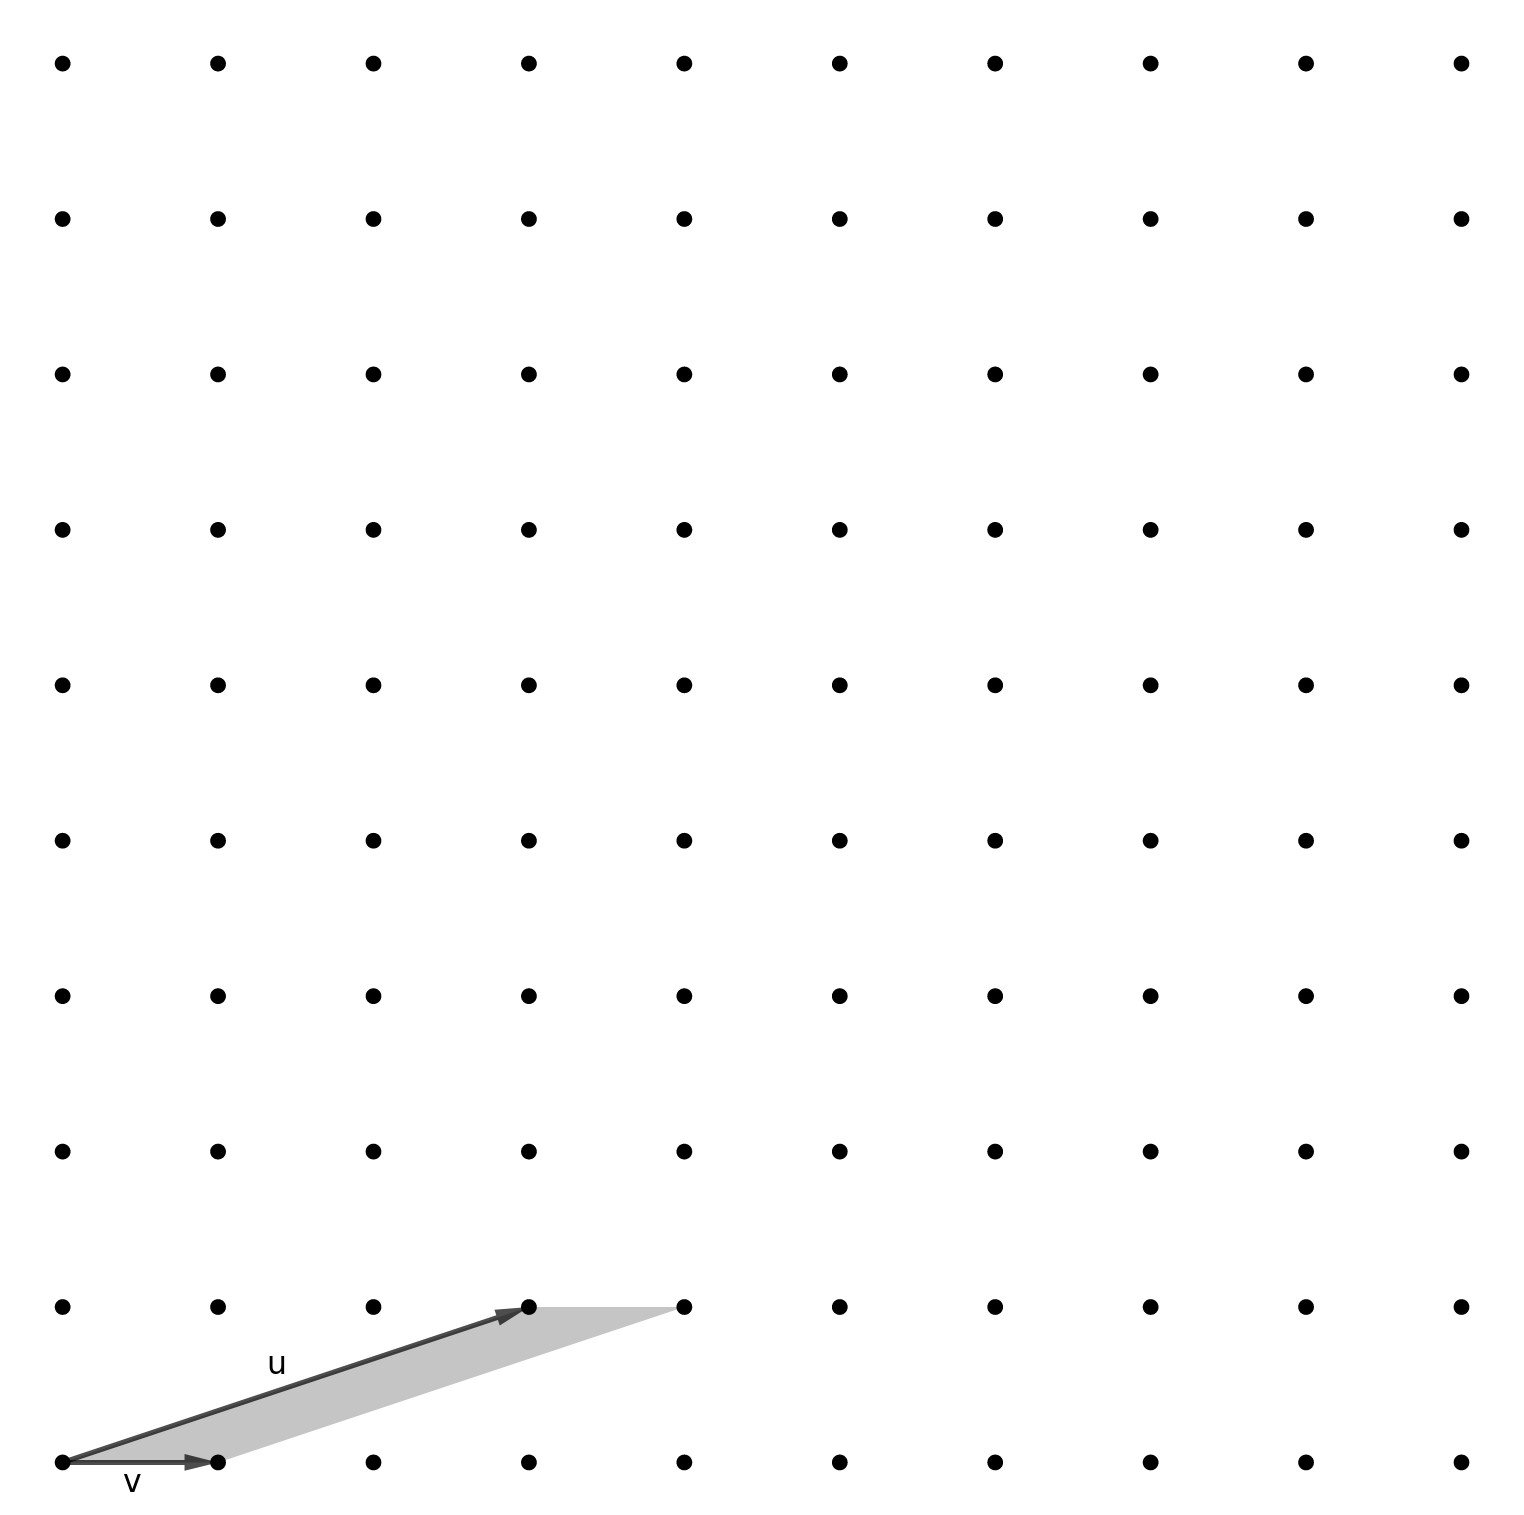
\includegraphics[width=0.75\textwidth]{Figuras/dominio_fundamental_2.png}\\
            \footnotesize{Fonte: O autor.}
        \end{minipage}
        \label{fig:dominio_fundamental_2}
    \end{figure}
    
    Sendo $\mathcal{L}$ um reticulado gerado por uma base $\textbf{B}$, o volume de seu domínio fundamental pode ser calculado pelo valor absoluto da determinante de $\textbf{B}$ na forma matricial, isto é:

    $$Vol(\mathcal{F}_B) = |Det(\textbf{B})|$$

    \noindent
    e também através do algoritmo de Gram Schmidt visto na Seção \ref{cap:reducao_base} por meio da seguinte equação segundo \cite{barros}:

    % = ou <=?
    $$Vol(\mathcal{F}_B) = \prod_{i=1}^{n} \Vert b_{i}^{*} \Vert$$

    \noindent
    em que $B$ é a base de um reticulado de dimensão $n$ e $b_{i}^{*}$ são os vetores gerados pelo algoritmo de Gram Schmidt da base $B$. Embora a base retornada pelo algoritmo de Gram Schmidt não gere o mesmo reticulado da base da entrada, ambas possuem o mesmo volume.

\section{Sucessivas mínimas}
    Seja $B_{n}(0, r) = \{x \in \mathbb{R}^{n}\ |\ ||x|| < r\}$ uma bola de dimensão $n$ centrada na origem e raio $r$. As sucessivas mínimas $\lambda_1, \lambda_2,...,\lambda_n$ de um reticulado $\mathcal{L}$ de dimensão $n$ são constantes, onde $\lambda_i(\mathcal{L})$ é o raio da menor bola de dimensão $i$ centrada na origem que contém $i$ vetores linearmente independentes de $\mathcal{L}$. As sucessivas mínimas de um reticulado $\mathcal{L}(\textbf{B})$  são definidas da seguinte forma:

    $$\lambda_i(\mathcal{L}) = min\{r\ |\ dim(\mathcal{L}(\textbf{B}) \cap \mathcal{B}(0, r)) \geq i  \}$$
    
    Tem-se na Figura \ref{fig:sucessive_minima} um reticulado de duas dimensões, isso significa que este reticulado tem apenas duas sucessivas mínimas $\lambda_1$ e $\lambda_2$. Analisando este reticulado da Figura \ref{fig:sucessive_minima}, a bola de dimensão 1 de menor raio e que contém um vetor linearmente dependente deste reticulado está destacada em uma cor mais escura e possui raio $\lambda_1$, e a bola de dimensão 2 de menor raio que contém os vetores linearmente independentes deste reticulado está destacada em uma cor mais clara e possui raio $\lambda_2$.

    Uma propriedade das sucessivas mínimas é que elas satisfazem $\lambda_1 \leq \lambda_2 \leq\ ...\  \leq \lambda_n$. Desta forma, $\lambda_1$ representa o tamanho do menor vetor de um reticulado com exceção do vetor nulo e também a menor distância entre dois elementos distintos desse reticulado \cite{daniele-lattices}.

    $$\lambda_1(\mathcal{L}) = \min_{x \neq y \in \mathcal{L}} ||x-y|| = \min_{x \in \mathcal{L} - {\vec{0}}} ||x||$$

    Alguns problemas baseados em reticulados estão relacionados com o menor vetor de um reticulado, também denotado por $\lambda_1$.
  
    \begin{figure}[htb!]
        \centering
        \caption{Sucessivas mínimas de um reticulado de duas dimensões.}
        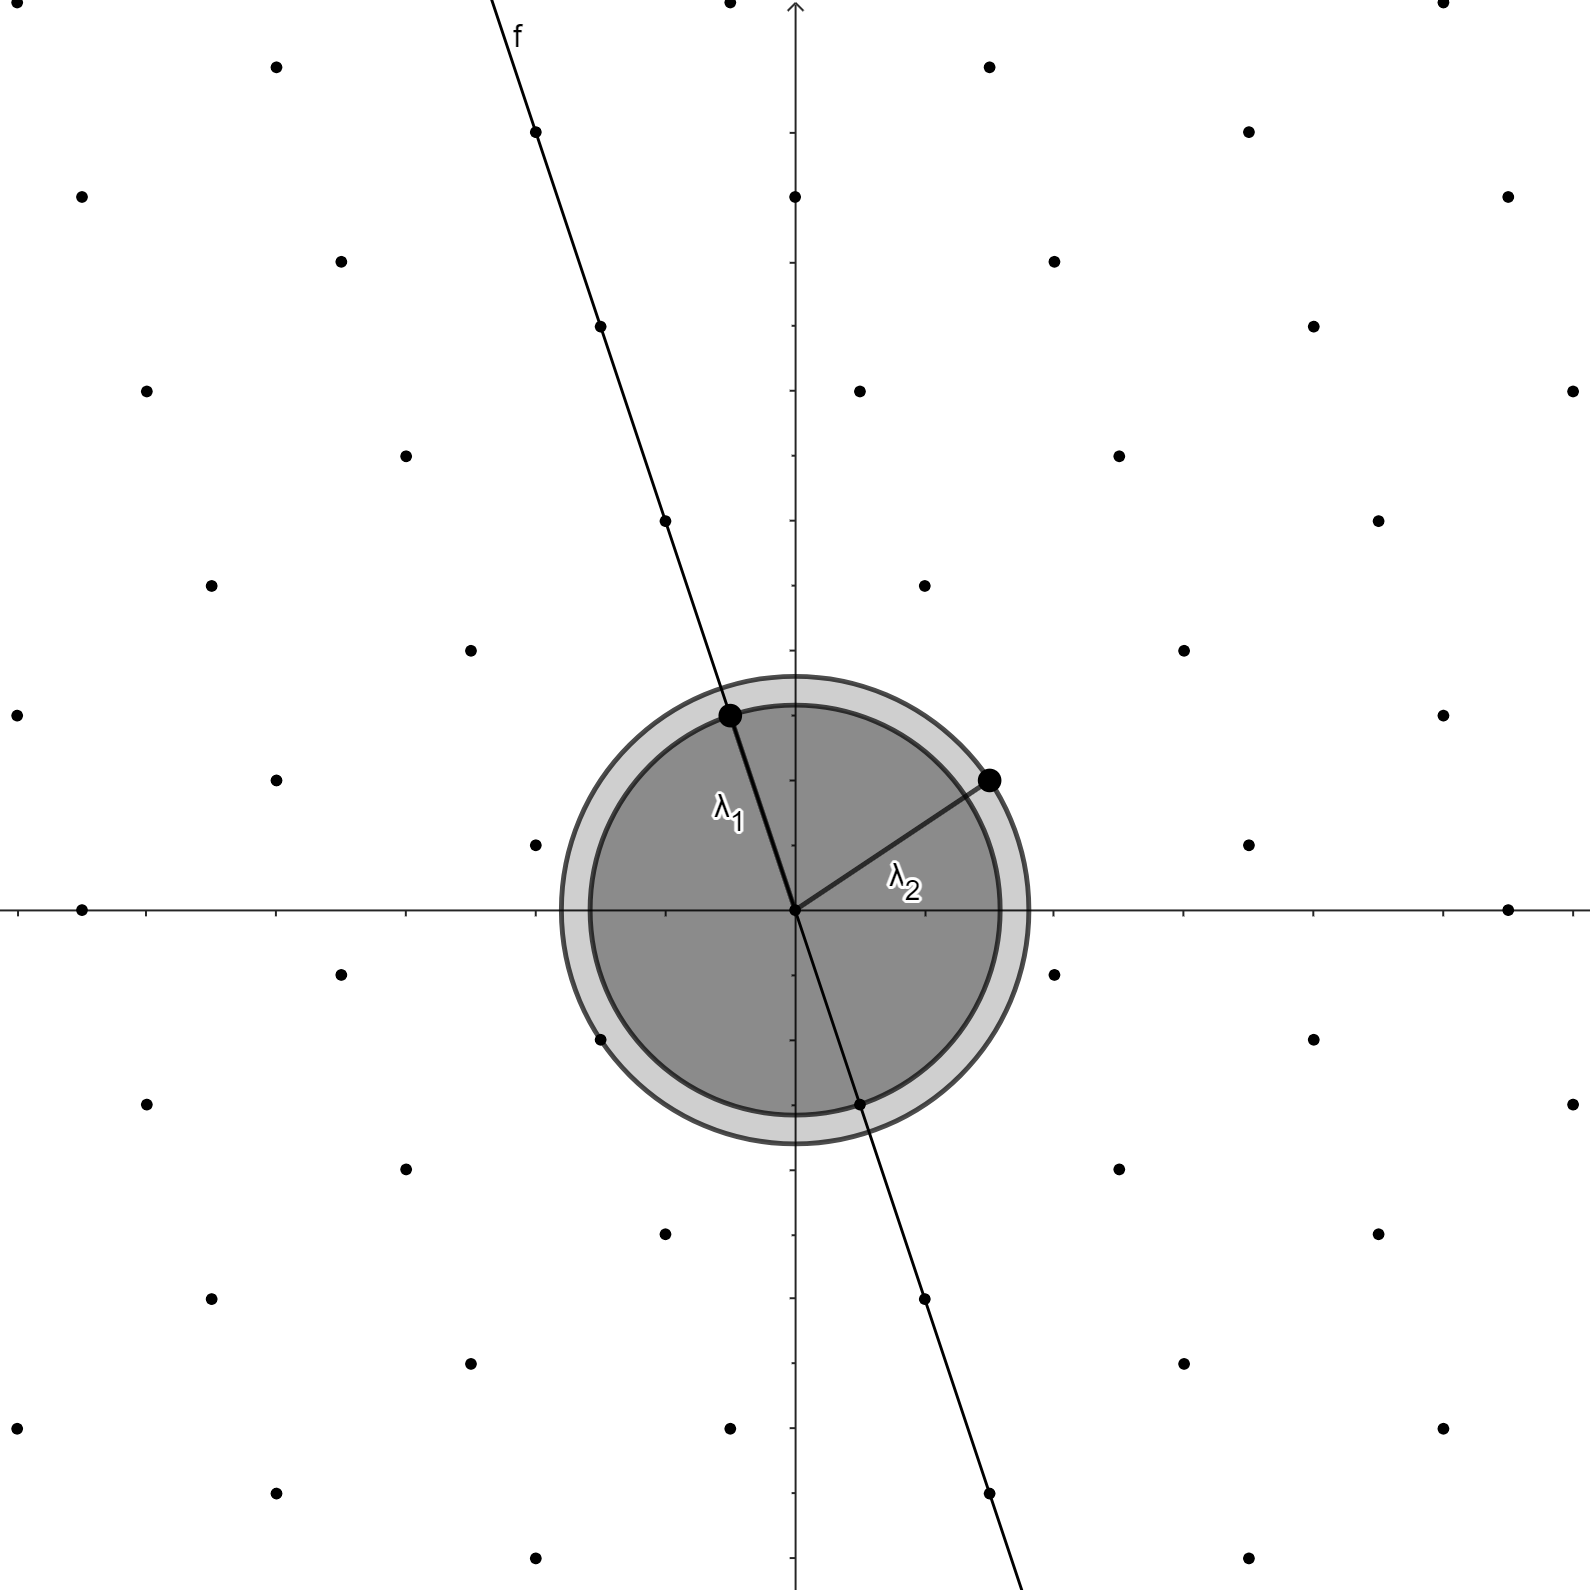
\includegraphics[width=0.75\textwidth]{Figuras/sucessive_minima.png}\\
        \footnotesize{Fonte: O autor.}
        \label{fig:sucessive_minima}
    \end{figure}
    
    As sucessivas mínimas de um reticulado dependem da métrica utilizada. Sejam os vetores $\vec{b_1} = \{2,0\}$ e $\vec{b_2} = \{1,1\}$, usando a métrica $l_1$ definida na Seção \ref{sec:espacos_metricos}, $\lambda_1 = \vec{b_1}$, visto que a norma de $\vec{b_1}$ sob a métrica $l_1$ é $2$. Entretanto, $\lambda_1 \neq \vec{b_1}$ se utilizadas as normas $l_2$ ou $l_{\infty}$ por exemplo. Isso se dá devido a $\vec{b_2}$ ser menor que $\vec{b_1}$ quando usadas essas métricas \cite{daniele-lattices}. Dessa forma, ao realizar uma análise de um problema computacional envolvendo sucessivas mínimas, deve-se ter bem definida qual métrica está sendo utilizada.

\section{Problemas computacionais}
\label{cap:lattice_problems}

%https://www.youtube.com/watch?v=o4Pl-0Q5-q0&ab_channel=SimonsInstitute -> EXPLICA MÉTODO SIEVING
%https://www.youtube.com/watch?v=LzWjLGG9cJI&ab_channel=TanjaLange%3APost-quantumcryptography -> EXPLICA MÉTODO ENUMERATION
%https://iacr.org/archive/crypto2007/46220170/46220170.pdf ->ENUMERATION
%https://math.mit.edu/~apost/courses/18.204-2016/18.204_Xinyue_Deng_final_paper.pdf -> LLL

%############################### TEM TUDO AQUIII #####################################
%#                    https://eprint.iacr.org/2012/533.pdf                           #
%#####################################################################################

%##################### IMPORTANTE PARA DEFIRNIR MODULAR LATTICES
%for any lattice B and point x ∈ span(B), there exists a unique vector y ∈ P(B) such that y − x ∈ L(B). This vector is denoted y = x mod B ->https://ieeexplore.ieee.org/document/1366257 

    
    Nesta seção serão apresentados alguns dos principais problemas computacionais sobre a estrutura de reticulados que formam a base da segurança dos sistemas de criptografia que utilizam esta estrutura. Como será visto nas Seções \ref{cap:algoritmos_exatos} e \ref{cap:reducao_base}, os algoritmos que resolvem estes problemas possuem complexidade exponencial ou pior, e os que executam em tempo polinomial conseguem apenas aproximações distantes do resultado ótimo para reticulados com certas propriedades, como dimensão, ortogonalidade e tamanho da norma dos vetores que formam a base do reticulado. Devido a este fato, os algoritmos que se baseiam nesses problemas são considerados seguros. 

    %https://dl.acm.org/doi/pdf/10.1145/237814.237838
    %The Complexity of Some Lattice Problems Jin-Yi Cai*
    %The Hardness of Approximate Optima in Lattices, Codes, and Systems of Linear Equations
    %danielle maciamicio
    
    \begin{definition}[\textit{Closest Vector Problem} (CVP)]
        O problema \ac{CVP} consiste em, dado um reticulado $\mathcal{L}$ e um vetor $\vec{c} \notin \mathcal{L}$, encontrar um vetor $\vec{v} \in \mathcal{L}$ tal que a distância entre $\vec{c}$ e $\vec{v}$ seja mínima.
    \end{definition}

    Intuitivamente, o problema \ac{CVP} pode ser aplicado à criptografia da seguinte maneira, seja $\vec{v} \in \mathcal{L(\beta)}$ uma chave privada, é somado a esta chave um vetor aleatório $\vec{e} \notin \mathcal{L(\beta)}$ com norma pequena, o resultado dessa soma é uma chave pública $\vec{c} \notin \mathcal{L(\beta)}$, dessa forma, para se recuperar a chave privada é preciso encontrar o vetor mais próximo de $\vec{c}$, que nesse caso seria a chave privada $\vec{v}$. Este é um dos principais problemas envolvendo reticulados e foi demonstrado por \cite{np-hard-cvp-svp} pertencer à classe dos problemas \ac{NP-HARD} para todas as normas $l_p$. A Figura \ref{fig:cvp} ilustra o problema \ac{CVP} em um reticulado de duas dimensões.
    
    \begin{definition}[\textit{Shortest Vector Problem} (SVP)]
         O problema \ac{SVP} consiste em, dado um reticulado $\mathcal{L}$, encontrar um vetor $\vec{v} \in \mathcal{L}$ tal que $\lVert \vec{v} \rVert$ seja mínima.
    \end{definition}

    Outro problema importante associado a reticulados é o problema \ac{SVP}, diferente do problema \ac{CVP}, este consiste em encontrar o vetor mais próximo da origem, que seria no caso o menor vetor do reticulado. Devido a essa relação com o problema \ac{CVP}, existe uma redução do problema \ac{SVP} para o \ac{CVP}, demonstrada em \cite{svp_to_cvp}. O problema \ac{SVP} foi demonstrado pertencer à classe \ac{NP-HARD} para a métrica $l_{\infty}$ por \cite{np-hard-cvp-svp}. A Figura \ref{fig:svp} ilustra este problema, em que $w$ é o vetor mais curto do reticulado.

    \begin{figure}[htb!]
        \begin{minipage}[c]{0.5\linewidth}
            \centering
            \caption{Ilustração do problema CVP.}
            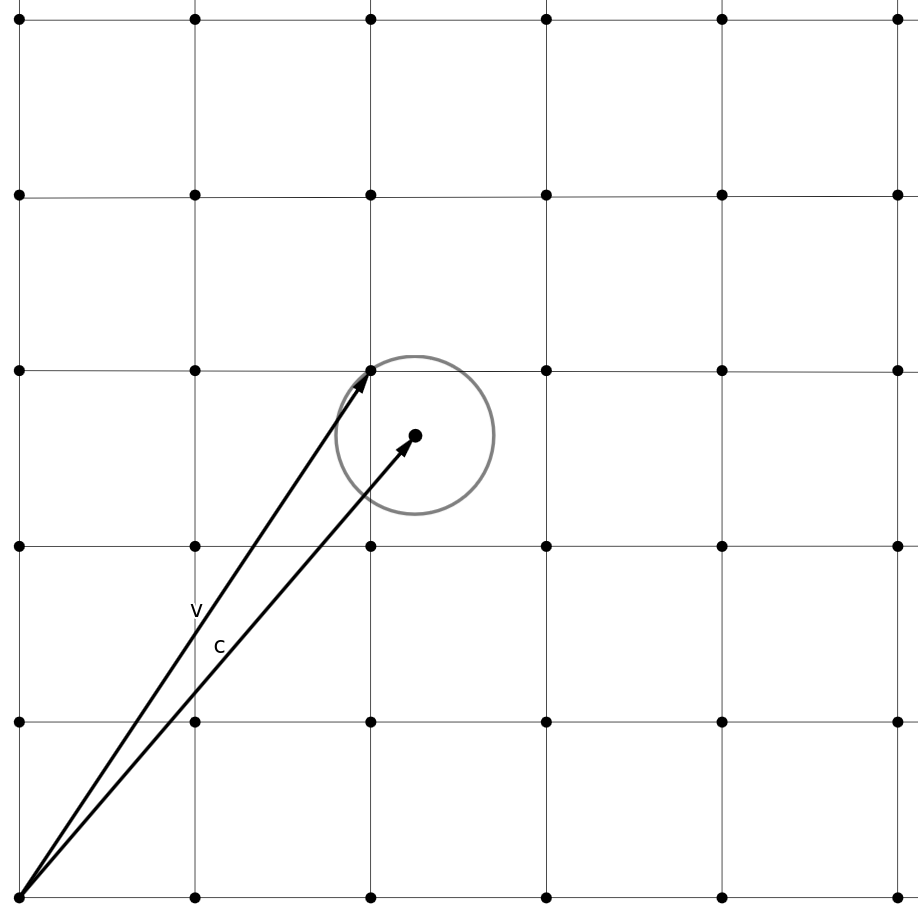
\includegraphics[width=0.75\textwidth]{Figuras/cvp.png}\\
            \footnotesize{Fonte: O autor.}
            \label{fig:cvp}
        \end{minipage}\hfill
        \begin{minipage}[c]{0.5\linewidth}
            \centering
            \caption{Ilustração do problema SVP.}
            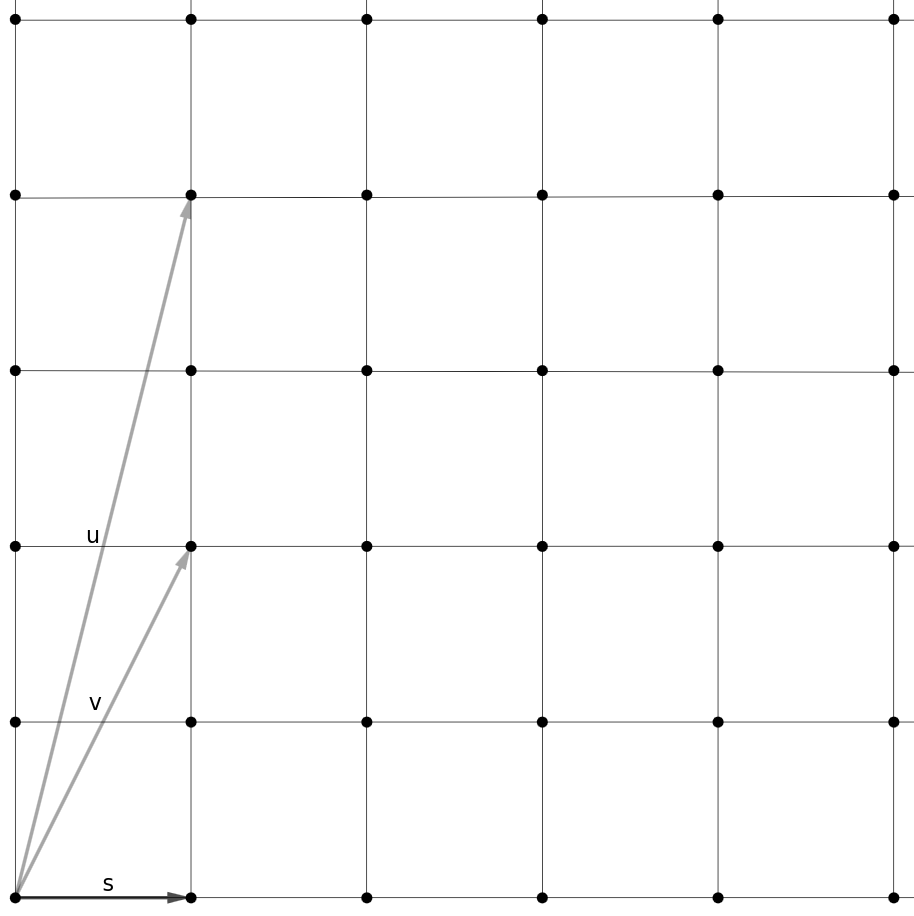
\includegraphics[width=0.75\textwidth]{Figuras/svp.png}\\
            \footnotesize{Fonte: O autor.}
            \label{fig:svp}
        \end{minipage}
    \end{figure}
    
    \begin{definition}[$CVP_\gamma$]
        O problema $CVP_\gamma$ consiste em dado um reticulado $\mathcal{L}$, um vetor $\vec{c} \notin \mathcal{L}$ e um fator de aproximação $\gamma \ge 1$, encontrar um vetor $v \in \mathcal{L}$ tal que $\|\vec{c} - \vec{v}\| \le \gamma d(\vec{c}, \mathcal{L})$.
    \end{definition}

    \begin{definition}[$SVP_\gamma$]
         O problema $SVP_\gamma$ consiste em, dado um reticulado $\mathcal{L}$ e um fator de aproximação $\gamma \ge 1$, encontrar um vetor $\vec{v} \in \mathcal{L}$ tal que $0 < \lVert \vec{v} \rVert \le \gamma \lambda_{1}(\mathcal{L})$. 
    \end{definition}

    Os problemas que utilizam um fator de aproximação, como $CVP_\gamma$ e $SVP_\gamma$, são estudados nos algoritmos que conseguem apenas uma aproximação do resultado ótimo para estes problemas. Esse fator geralmente está em função do grau do reticulado, por exemplo $\gamma(n) = (2 / \sqrt{3})^n$, isso significa que o resultado desse algoritmo estará no máximo a $\gamma$ de distância do resultado ótimo. Os algoritmos que resolvem uma aproximação desses problemas se encontram na Seção \ref{cap:reducao_base}.

     \begin{definition}[\textit{Gap Shortest Vector Problem} ($GapSVP_\gamma$)]
        O problema $GapSVP_\gamma$ consiste em, dado um reticulado $\mathcal{L}$ e um número real positivo $d$, determinar se $\lambda_1(\mathcal{L}) \leq d$ ou $\lambda_1(\mathcal{L}) > \gamma d$.
    \end{definition}

    \begin{definition}[\textit{Shortest Independent Vector Problem} ($SIVP_\gamma$)]
        O problema $SIVP_\gamma$ consiste em, fornecido um reticulado $\mathcal{L}$ de dimensão $n$, encontrar um conjunto de $n$ vetores linearmente independentes com comprimento máximo de $\gamma \lambda_{n}(\mathcal{L})$.
    \end{definition}
    
    \begin{definition}[\textit{Learning With Errors} (LWE)]
        Dado uma matriz $\textbf{A} \in \mathbb{Z}_p^{m \times n}$ gerada por uma distribuição de probabilidade uniforme e uma matriz $\textbf{t} = \textbf{As} + \textbf{e} \in \mathbb{Z}_p^m$, sendo $\textbf{e} \in \mathbb{Z}_p^m$ um erro adicional especificado por uma distribuição de probabilidade $\chi:\mathbb{Z}_p \to \mathbb{R}^{+}$ em $\mathbb{Z}_p$, encontrar a matriz $\textbf{s} \in \mathbb{Z}_p^n$ \cite{regev}. 
    \end{definition}

    \begin{figure}[htb!]
        \centering
        \caption{Ilustração do problema \ac{LWE}.}
        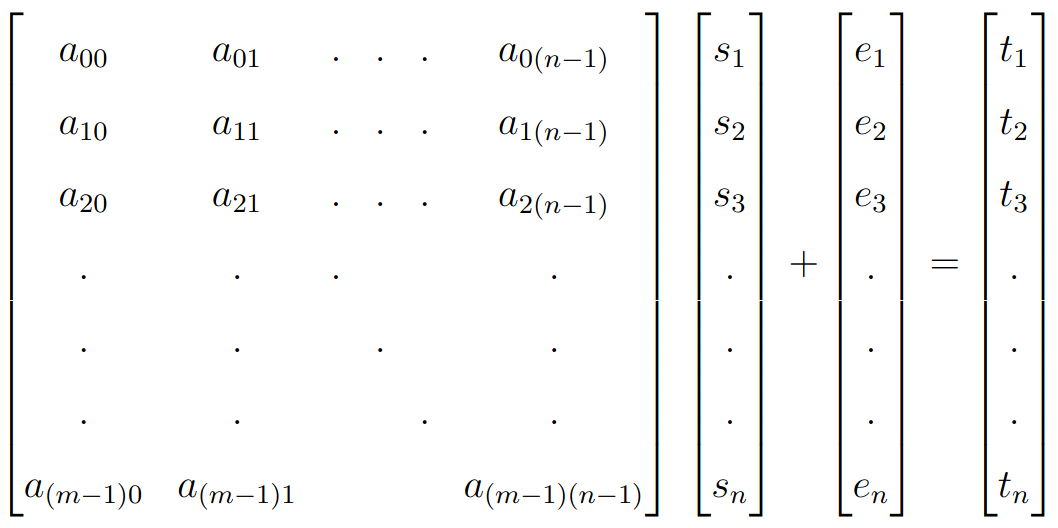
\includegraphics[width=0.65\textwidth]{Figuras/lwe.png}\\
        \footnotesize{Fonte: O autor.}
        \label{fig:lwe}
    \end{figure}

    O problema \ac{LWE} foi introduzido por \cite{regev} e consiste na dificuldade de se obter a solução para uma equação linear com um erro, como pode ser observado na Figura \ref{fig:lwe}. Perceba que sem a matriz de erro/ruído \textbf{e}, este problema poderia ser facilmente resolvida pela eliminação Gaussiana em tempo $\mathcal{O}(n)$, sendo $n$ o número de equações a serem resolvidas. Entretanto, se adicionarmos um erro aleatório a essa equação, resolvê-la é uma tarefa difícil, até para computadores quânticos. O artigo \cite{regev} relata a dificuldade de se encontrar algoritmos clássicos e quânticos que resolvem este problema em tempo polinomial, o que o torna útil para a criação de sistemas de criptografia baseados neste problema. A complexidade de resolução do \ac{LWE} está relacionada com a dificuldade de resolução dos problemas \ac{GapSVP} e \ac{SIVP}, visto que \cite{regev} demonstra uma redução destes problemas para \ac{LWE}.

    Este problema, além de ser seguro contra computadores quânticos, chamou atenção devido a sua versatilidade, eficiência e simplicidade. Ele foi a base para a criação de outros problemas computacionais como \ac{RLWE}, \ac{MLWE} e também outros modelos de criptografia, como criptografia homomórfica.

    Um aspecto a ser considerado ao utilizar o \ac{LWE} é o tamanho da chave pública, representado pela matriz \textbf{A}. Em que a complexidade de espaço é $\mathcal{O}(n^2)$, sendo $n$ a ordem da matriz \textbf{A}. Esta é uma das razões pela qual este problema não é utilizado na prática em sistemas criptográficos. O problema \textit{Ring Learning With Errors} (RLWE) apresenta uma alternativa para diminuir o tamanho da matriz \textbf{A} e melhorar o desempenho das operações de multiplicação matricial devido à seguinte relação:

        \begin{center}
            $\begin{bmatrix}
                b_{1}   & -b_{n}   & -b_{n-1} & . & . & . & -b_{2}\\
                b_{2}   &  b_{1}   & -b_{n-2} & . & . & . & -b_{3}\\
                b_{3}   &  b_{2}   &  b_{1}   & . & . & . & -b_{4}\\
                .       & .        &          & . & . & . & .     \\
                .       & .        &          &   & . & . & .     \\
                .       & .        &          &   &   & . & .     \\
                b_{n} & b_{n-1}&              &   &   &   & b_{1}
            \end{bmatrix}$
            %
            $\begin{bmatrix}
                s_1  \\
                s_2  \\
                s_3  \\
                .    \\
                .    \\
                .    \\
                s_{n}
            \end{bmatrix}$
            %
            $\Leftrightarrow$
            %
            $(b_1 + b_2 x + b_3 x^2 + ... + b_{n} x^{n-1})(s_1 + s_2 x + s_3 x^2 + ... + s_{n} x^{n-1})\ \textbf{mod}\ x^n + 1$
        \end{center}
    
    Dessa forma é possível obter os demais elementos da matriz a partir da primeira coluna, sendo assim, necessário apenas armazenar a primeira coluna, o que resulta em uma diminuição do tamanho da chave criptográfica. 
    
    \begin{definition}[\textit{Ring Learning With Errors} (RLWE)]
        Seja $A \in \mathbb{Z}_q{[}x{]} / \langle x^n+1 \rangle$ gerada por uma distribuição de probabilidade uniforme e um polinômio $t = As + e \in \mathbb{Z}_q{[}x{]} / \langle x^n+1 \rangle$ sendo $e \in \mathbb{Z}{[}x{]} / \langle x^n+1 \rangle$ especificado por uma distribuição de probabilidade $\chi$ em $\mathbb{Z}{[}x{]} / \langle x^n+1 \rangle$ com desvio padrão $\sigma$, considerando-o em $\mathbb{Z}_q{[}x{]} / \langle x^n+1 \rangle$, encontrar o polinômio $s \in \mathbb{Z}_q{[}x{]} / \langle x^n+1 \rangle$ \cite{ring_lwe}. 
    \end{definition}
    
    A redução do tamanho da chave não é a única vantagem oferecida pelo \ac{RLWE}, transformando os vetores $\vec{b}$ e $\vec{s}$ em polinômios através do isomorfismo $\sigma_1:P[x] \to \mathbb{Z}^n$, a multiplicação entre $\sigma_{1}^{-1}(\vec{b})$ e $\sigma_{1}^{-1}(\vec{s})$ módulo $x^n + 1$ é equivalente à multiplicação matricial acima. A realização de uma operação de multiplicação polinomial modular, em vez da matricial, proporciona aceleração à operação de multiplicação por meio do algoritmo \ac{NTT} \cite{ntt}, onde a complexidade passa a ser $\mathcal{O}(n log(n))$. A redução do tamanho da chave, segundo \cite{ring_lwe}, não reduz a complexidade do problema, desde que se escolha os parâmetros $\sigma$, $n$ e $q$ adequadamente.
    
    \begin{definition}[\textit{Module Learning With Errors} (MLWE)]
        Seja $\textbf{A} \in {[}\mathbb{Z}_q{[}x{]} / \langle x^n+1 \rangle{]}^{m \times k}$ gerada por uma distribuição de probabilidade uniforme e uma matriz $\textbf{t} = \textbf{As} + \textbf{e} \in {[}\mathbb{Z}_q{[}x{]} / \langle x^n+1 \rangle{]}^{m}$ sendo $\textbf{e} \in {[}\mathbb{Z}_q{[}x{]} / \langle x^n+1 \rangle{]}^{m}$, encontrar a matriz $\textbf{s} \in {[}\mathbb{Z}_q{[}x{]} / \langle x^n+1 \rangle{]}^{k}$ \cite{module-lwe}. 
    \end{definition}

    \begin{figure}[htb!]
        \centering
        \caption{Ilustração do problema \ac{MLWE}.}
        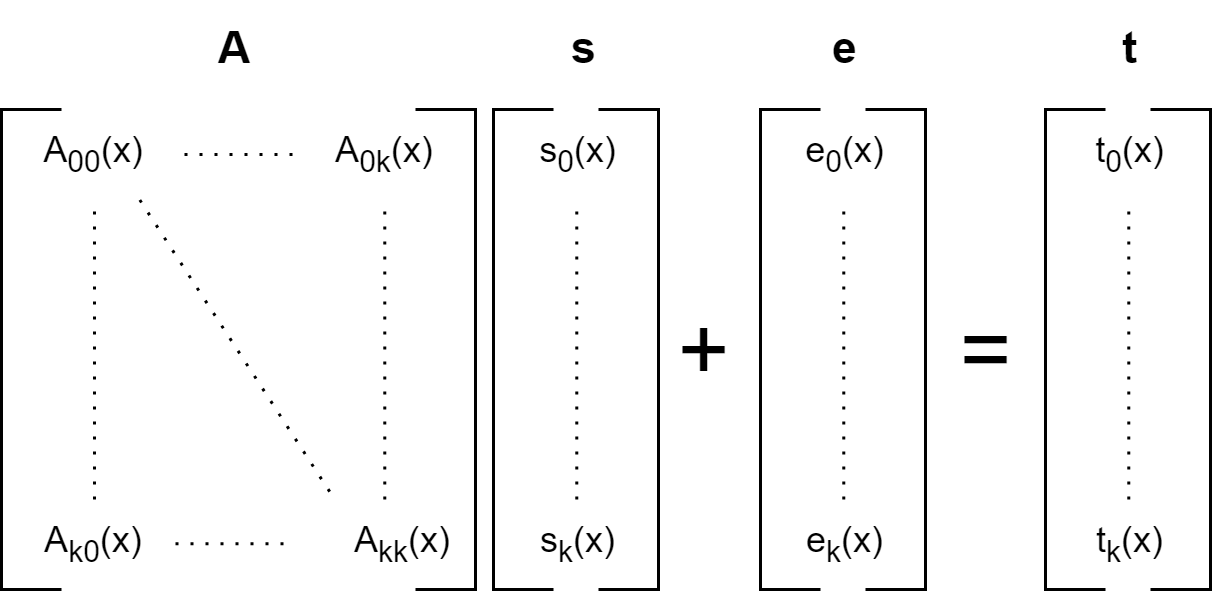
\includegraphics[width=0.75\textwidth]{Figuras/kyber_keygen.png}\\
        \footnotesize{Fonte: O autor.}
        \label{fig:mlwe}
    \end{figure}

    O problema \ac{MLWE} é semelhante ao problema \ac{LWE} como pode ser observado na Figura \ref{fig:mlwe}, com a diferença que os elementos das matrizes, em vez de inteiros, agora são polinômios. O \ac{MLWE} pode ser interpretado como vários problemas \ac{RLWE} dentro do \ac{LWE}, visto que se alterado o parâmetro $k$ para 1, tem-se exatamente o problema \ac{RLWE}. Segundo a documentação oficial do \ac{ML-KEM} \cite{kyber}, os autores optaram por utilizar o \ac{MLWE} por preocupações que a estrutura \ac{RLWE} possa permitir ataques mais eficientes, além de que o \ac{MLWE} possui uma melhor escalabilidade e eficiência semelhante ao \ac{RLWE} para determinados parâmetros \cite{kyber2}.

\section{Algoritmos exatos}
\label{cap:algoritmos_exatos}
    Existem duas técnicas que resolvem com exatidão os problemas SVP e CVP, a técnica de \textit{sieving} e a técnica de \textit{enumeration}. 
    
    A técnica de \textit{sieving} foi proposta pela primeira vez em 2001 por Miklós Ajtai, Ravi Kumar e D. Sivakumar \cite{sieving}, e existem diversas variações deste algoritmo com complexidade de tempo inferior ao algoritmo original $\mathcal{O}(2^n)$, porém ainda com complexidade exponencial de tempo e espaço, o que torna estes algoritmos impraticáveis para reticulados de grandes dimensões. A ideia principal desta técnica é selecionar um conjunto de vetores em uma região de raio $R$ de um reticulado, realizar sucessivas subtrações entre pares de vetores deste conjunto e adicionar os vetores resultantes dessas operações ao conjunto final caso sua norma for menor que $\gamma R$ para $0< \gamma < 1$. A Figura \ref{fig:sieving} ilustra a ideia-chave dos algoritmos que utilizam a técnica de \textit{sieving}. 

    \begin{figure}[htb!]
        \centering
        \caption{Exemplo do funcionamento do algoritmo \textit{sieving} com duas iterações respectivamente.}
            \begin{subfigure}{.5\textwidth}
                \centering
                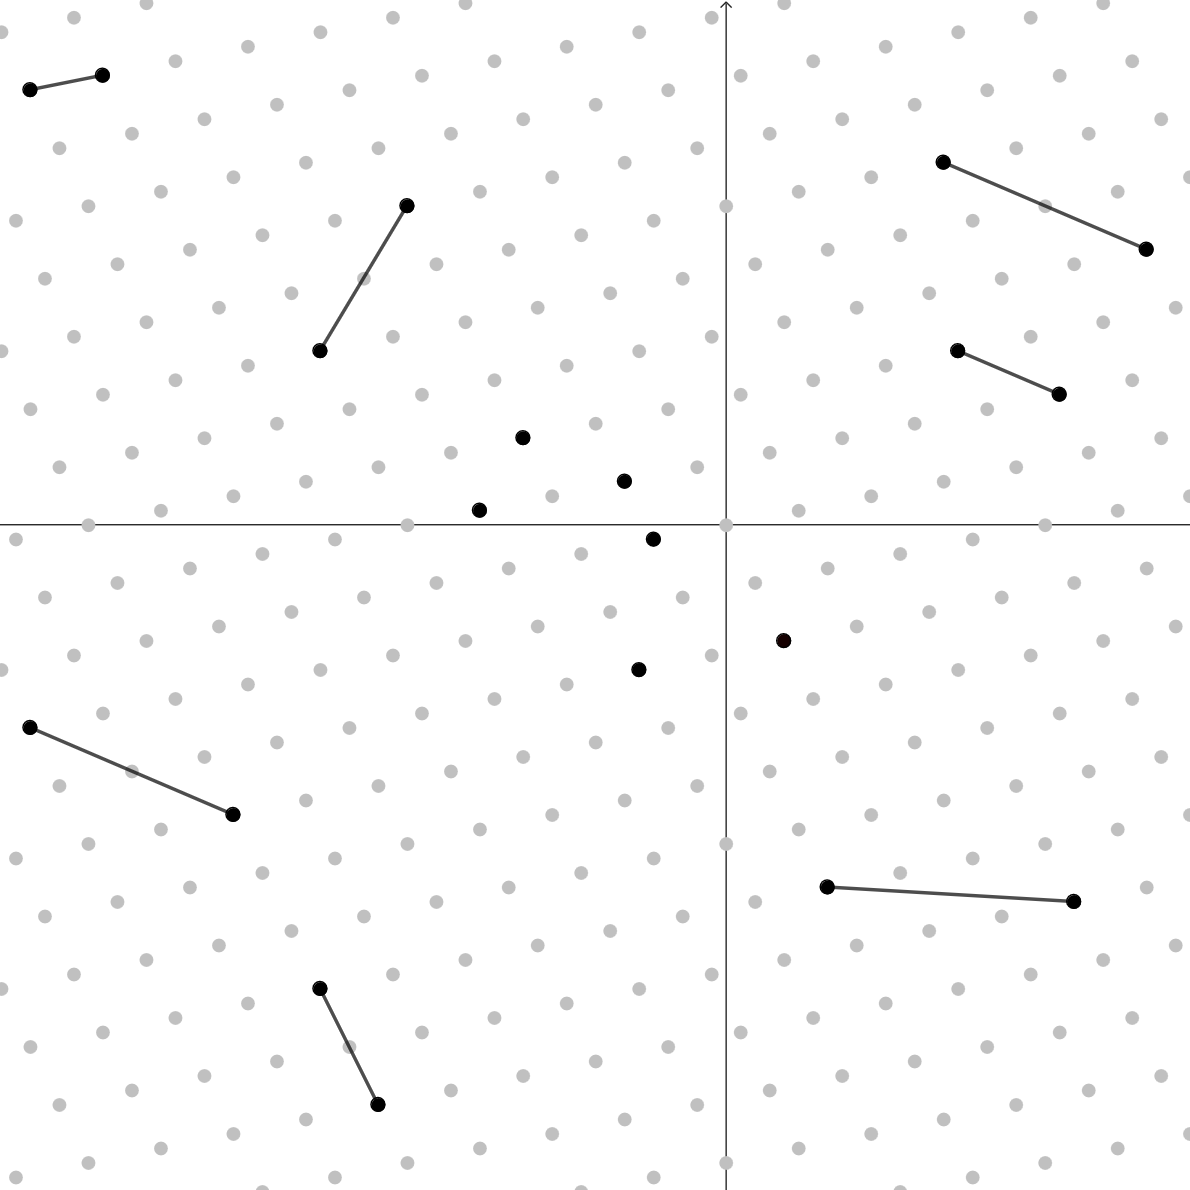
\includegraphics[width=.75\linewidth]{Figuras/sieving_1.png}
            \end{subfigure}%
            \begin{subfigure}{.5\textwidth}
                \centering
                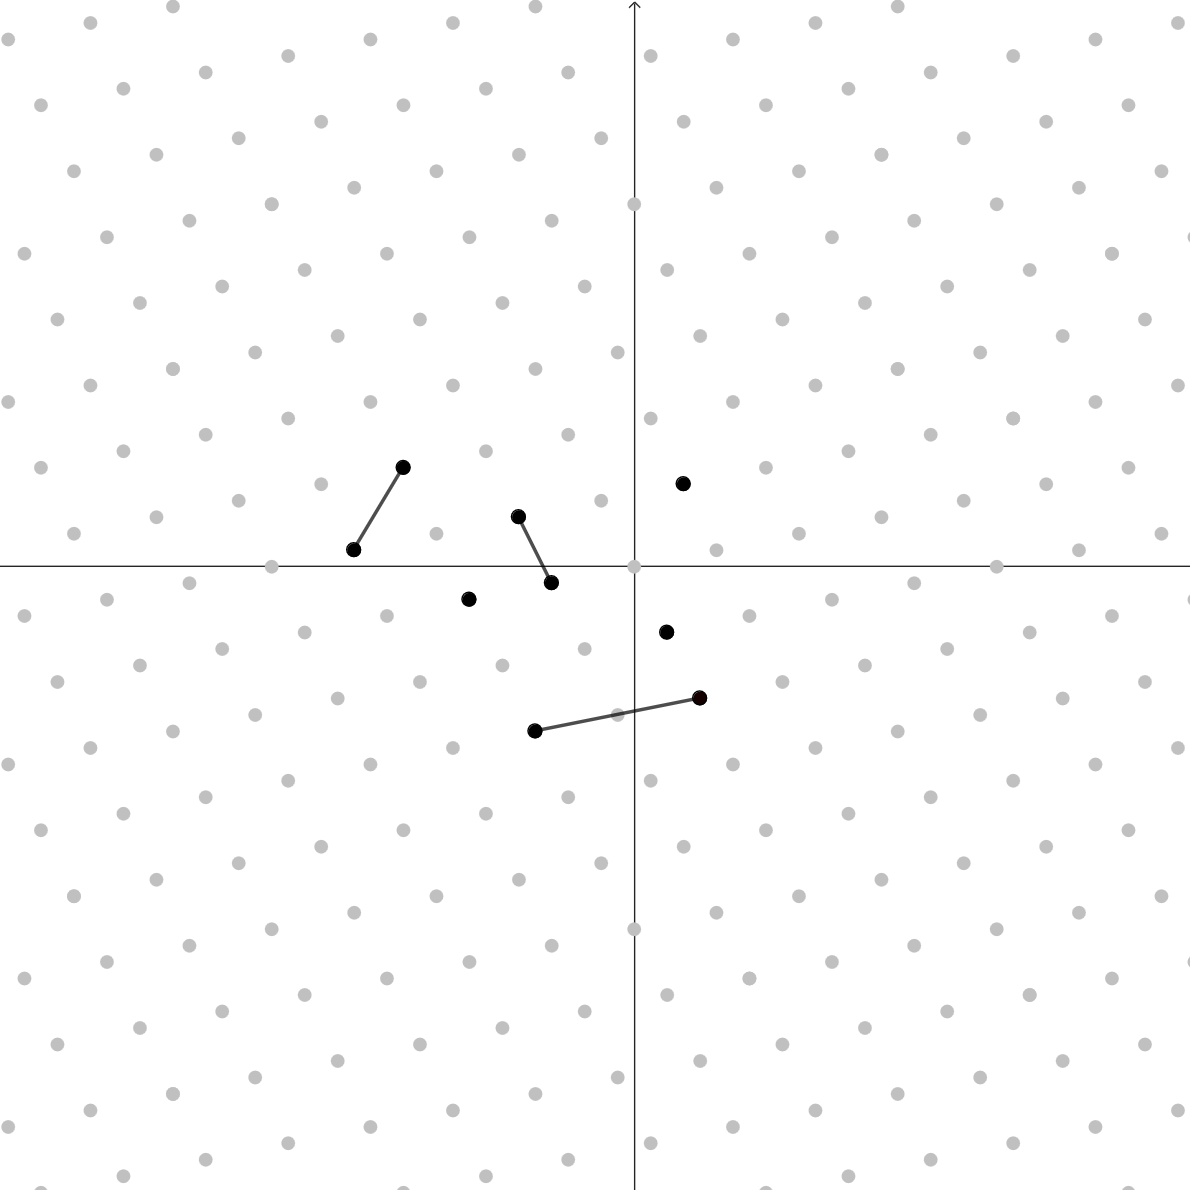
\includegraphics[width=.75\linewidth]{Figuras/sieving_2.png}
            \end{subfigure}
        \footnotesize{Fonte: O autor.}
        \label{fig:sieving}
    \end{figure}

    %https://sci-hub.se/http://dx.doi.org/10.1090/S0025-5718-1985-0777278-8
    A técnica de \textit{enumeration} foi proposta pela primeira vez por U. Fincke e M. Pohst em 1985 \cite{enumeration_fincke_pohst}, entretanto, devido à sua complexidade de $\mathcal{O}(2^{n^2})$, é mais conhecido o algoritmo proposto por Ravi Kannan de 1987, com complexidade de $\mathcal{O}(n^n)$ \cite{enumeration_kannan}. Este algoritmo, assim como o AKS, também resolve o problema SVP com exatidão, e embora possua complexidade de tempo maior que o algoritmo AKS $\mathcal{O}(n^n)$, este algoritmo tem a vantagem de possuir complexidade polinomial de espaço. A ideia principal dos algoritmos de \textit{enumeration} é selecionar duas bases $\vec{b_1}$ e $\vec{b_2}$, calcular a projeção de $\vec{b_2}$ sobre a reta ortogonal a $\vec{b_1}$. O próximo passo é enumerar os vetores em uma região que estão a uma distância múltipla da norma do vetor resultante da projeção de $\vec{b_2}$ sobre a reta ortogonal a $\vec{b_1}$. A partir destes vetores enumerados o algoritmo de Kannan encontra o vetor mais curto nesta região. A Figura \ref{fig:lattice_enumeration} ilustra este processo, onde os pontos destacados são os vetores enumerados pelo algoritmo.

    \begin{figure}[htb!]
        \centering
        \caption{Exemplo do funcionamento do algoritmo \textit{enumeration}.}
        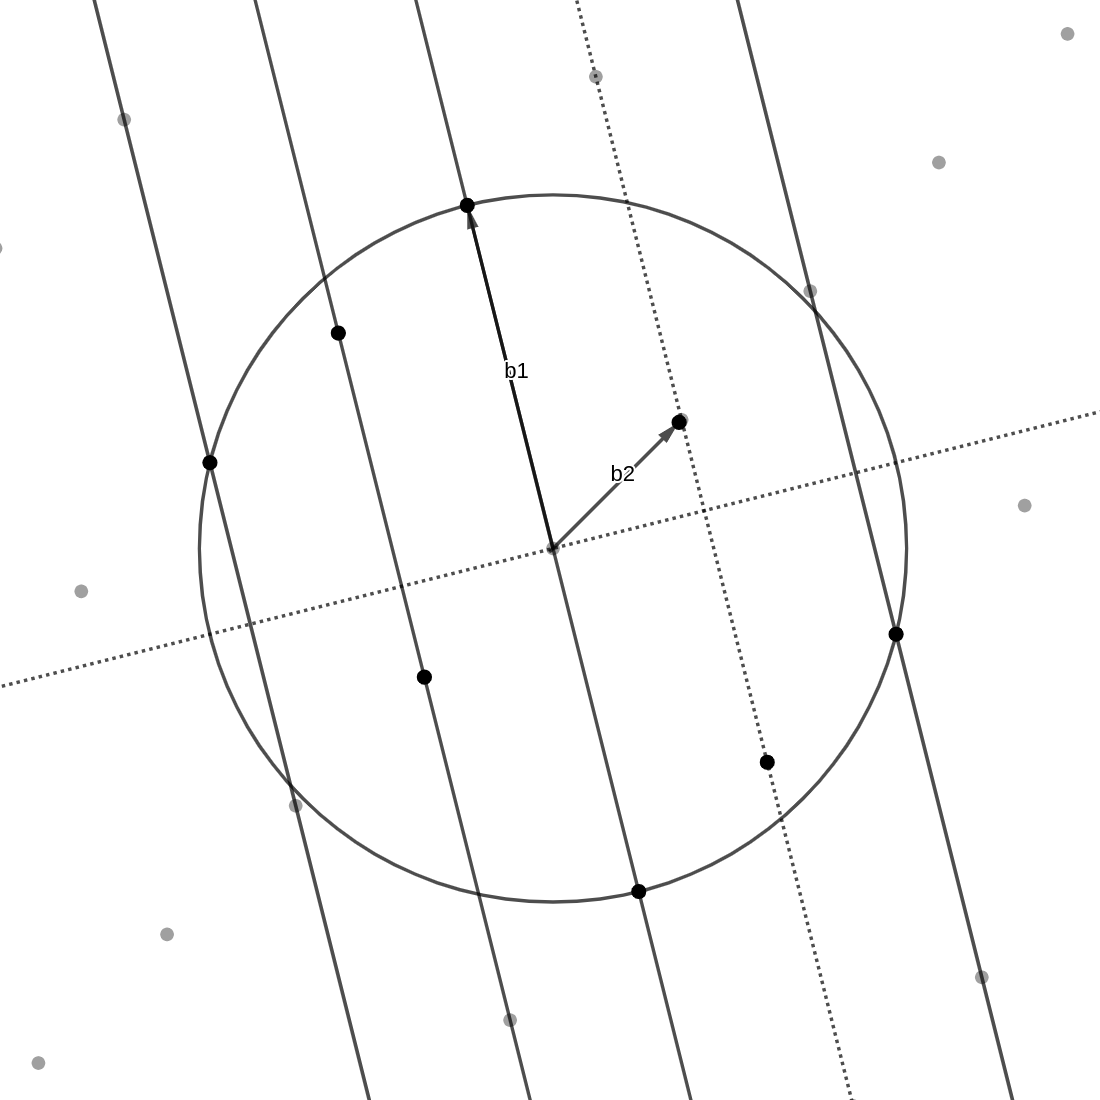
\includegraphics[width=0.65\textwidth]{Figuras/lattice_enumeration.png}\\
        \footnotesize{Fonte: O autor.}
        \label{fig:lattice_enumeration}
    \end{figure}

\section{Redução de base}
\label{cap:reducao_base}
%http://www.noahsd.com/mini_lattices/05__babai.pdf -> algoritmo de babai, intepretação geométrica
    A segurança dos algoritmos baseados em problemas envolvendo reticulados está relacionada com algumas propriedades da base do reticulado, mais especificamente a ortogonalidade, norma e dimensão dos vetores da base. A técnica de redução de base de um reticulado consiste em encontrar outra base que gere este mesmo reticulado, mas com vetores com a menor norma possível e mais ortogonais entre si. É possível calcular a ortogonalidade da base de um reticulado pela \textit{Razão de Hadamard}, esta é dada pela fórmula
    
    $$ \mathcal{H}(\beta) = \left( \frac{|Det(\textbf{B})|}{ \prod_{i=1}^{n} ||b_i||  } \right)^\frac{1}{n} $$

    \noindent
    em que $0 < \mathcal{H}(\textbf{B}) \leq 1$\cite{barros}. Quanto mais próximo de 1 for $\mathcal{H}(\textbf{B})$, mais ortogonal é a base $\textbf{B}$, esta é dita uma base boa, enquanto para uma base ruim os valores de $\mathcal{H}(\textbf{B})$ se aproximam de 0.
    
    \begin{figure}[htb!]
        \begin{minipage}[c]{0.5\linewidth}
            \centering
            \caption{Exemplo de uma base boa.}
            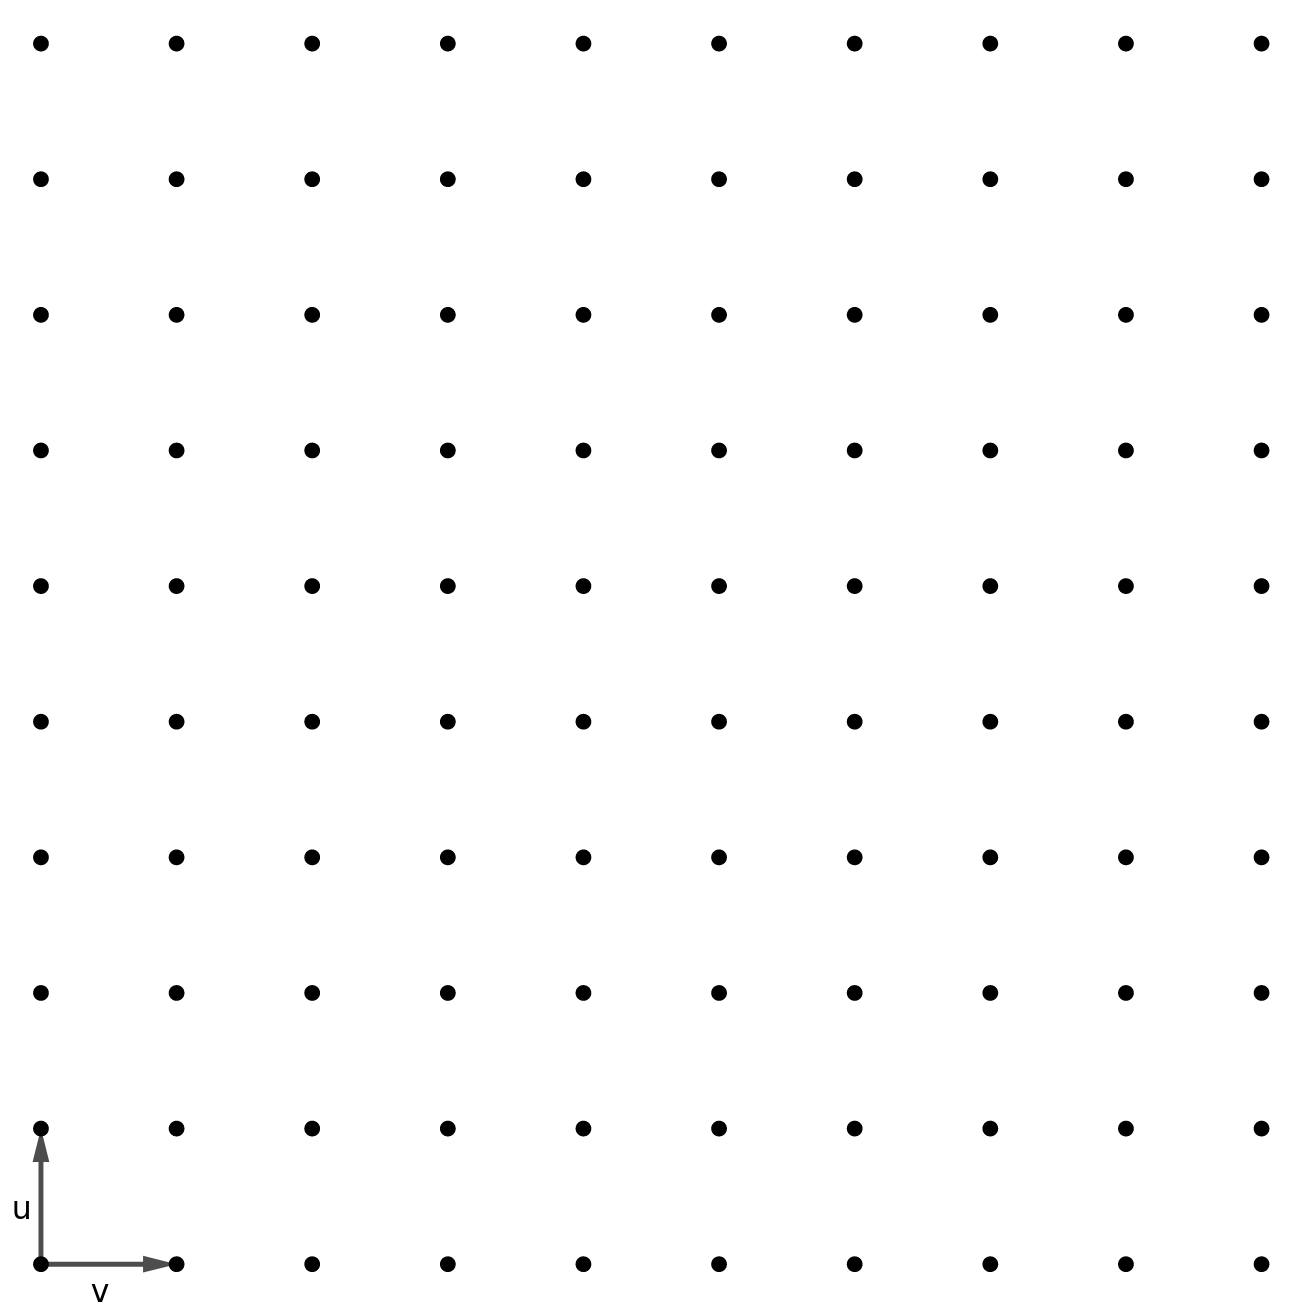
\includegraphics[width=0.75\textwidth]{Figuras/base_boa.png}\\
            \footnotesize{Fonte: O autor.}
            \label{fig:base_boa}
        \end{minipage}\hfill
        \begin{minipage}[c]{0.5\linewidth}
            \centering
            \caption{Exemplo de uma base ruim.}
            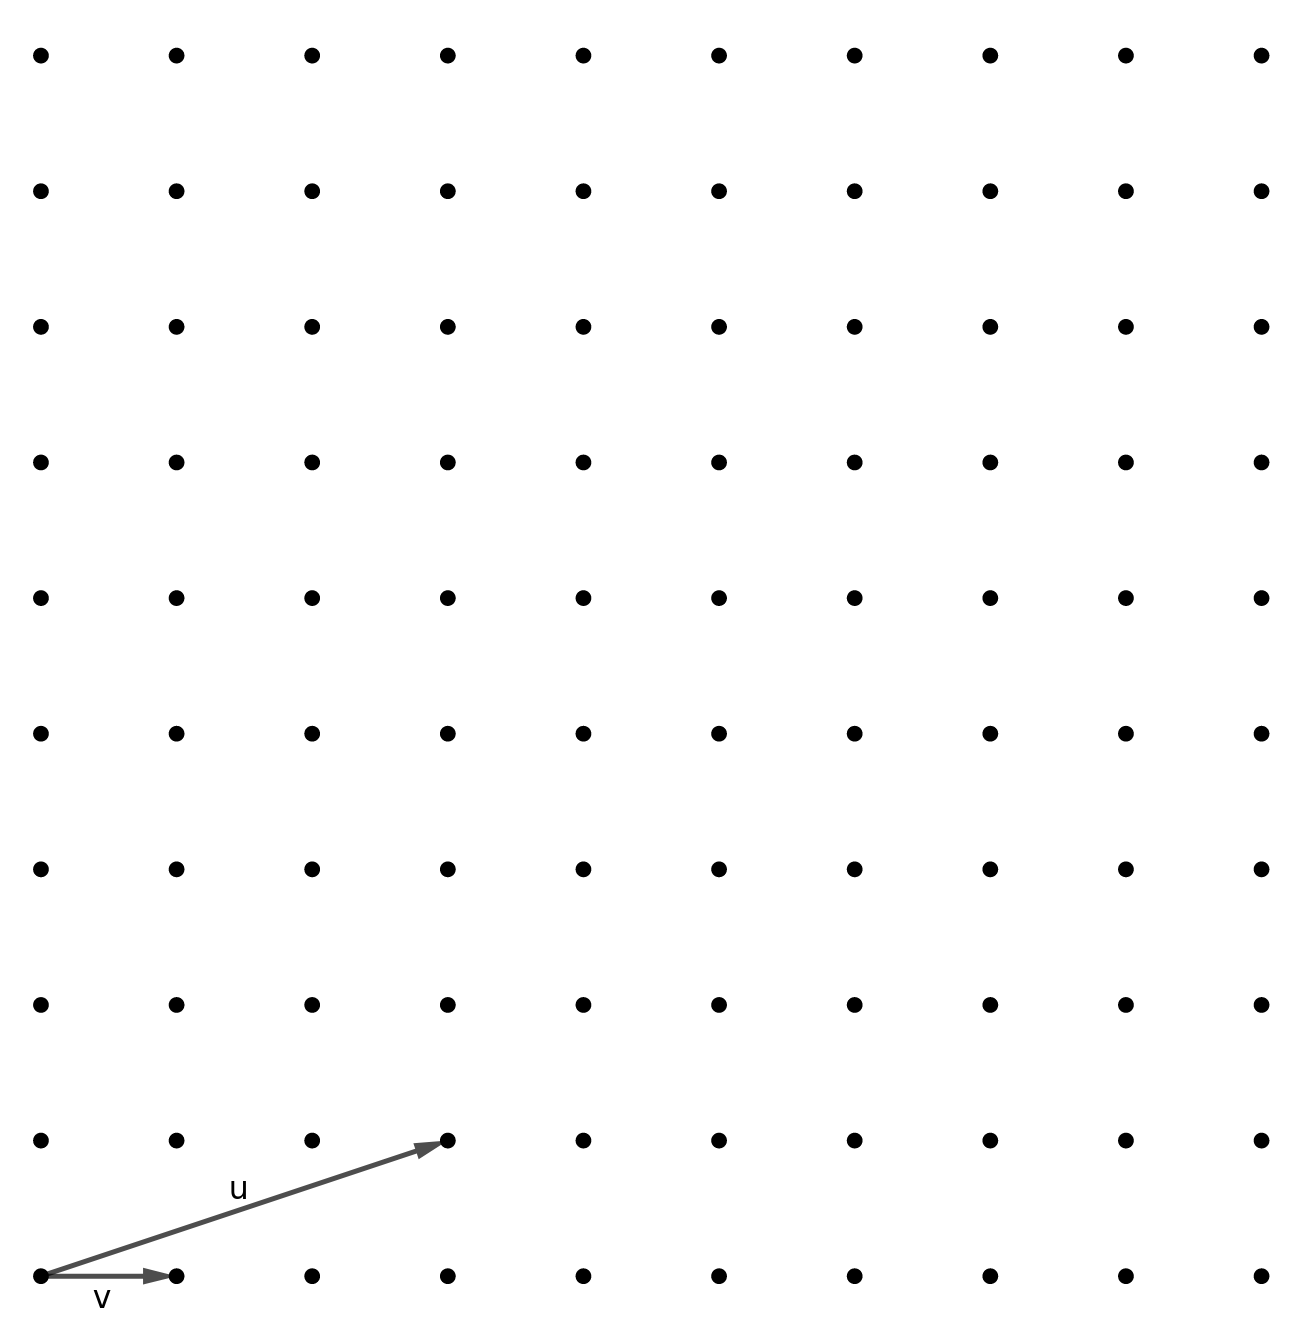
\includegraphics[width=0.75\textwidth]{Figuras/base_ruim.png}\\
            \footnotesize{Fonte: O autor.}
            \label{fig:base_ruim}
        \end{minipage}
    \end{figure}

    Os reticulados das Figuras \ref{fig:base_boa} e \ref{fig:base_ruim}, embora gerados por vetores completamente diferentes, são iguais tendo em vista que os vetores que geram o reticulado da Figura \ref{fig:base_ruim} podem ser expressos por uma combinação linear dos vetores que geram o reticulado da Figura \ref{fig:base_boa}. Entretanto, a base da Figura \ref{fig:base_boa}, gerada pelos vetores $\{(1,0),(0,1)\}$ é uma base boa, pois os vetores são ortogonais entre si e possuem sua norma pequena, a prova disso é o cálculo da \textit{Razão de Hadamard} da base, que é exatamente $1$. Já a base da Figura \ref{fig:base_ruim} é considerada ruim, visto que a \textit{Razão de Hadamard} é aproximadamente $0{,}56$. A base ser boa implica que conseguiremos boas aproximações pelos algoritmos de redução de base que serão abordados na seção \ref{algoritmos_reducao_base}.

    \subsection{Algoritmos de redução de base}
    \label{algoritmos_reducao_base}
        A razão pela qual deseja-se uma base reduzida, é para se obter uma boa aproximação para o problema \ac{CVP} através do algoritmo de Babai. O algoritmo de Babai \cite{babai} proposto em 1985 por László Babai, realiza uma aproximação da solução do problema CVP dada uma base boa, na qual este funciona da seguinte maneira:
        
        \begin{enumerate}
            \item Sendo $\vec{s} \notin \mathcal{L(\beta)}$, escreva $\vec{s}$ como uma combinação linear de $\beta$;
            \item Os coeficientes da combinação linear devem ser arredondados para um inteiro mais próximo;
            \item Os coeficientes arredondados combinados com a base devem gerar uma aproximação do vetor mais próximo de $\vec{s}$ que pertence à $\mathcal{L(\beta)}$.
        \end{enumerate}
        
        Esse algoritmo realiza uma boa aproximação do problema \ac{CVP} ao ter uma base bem ortogonal, do contrário, o resultado não é preciso. Tenha como exemplo um reticulado $\mathcal{L}(\beta)$ gerado pela base $\beta = \{ (5,1),(-2,8) \}$ e um vetor $\vec{s} = (27,8) \notin \mathcal{L}(\beta)$. A \textit{Razão de Hadamard} de $\beta$ é $\mathcal{H}(\beta) \thickapprox 0.999$, isso significa que devemos obter uma boa aproximação. Ao realizarmos os cálculos, obtém-se o vetor $\vec{c} = (30, 6)$, sendo relativamente próximo de $\vec{s}$. Agora, aplicando o algoritmo de Babai para outra base $\beta = \{(37,41),(103,113)\}$ menos ortogonal que gera o mesmo reticulado, em que  $\mathcal{H}(\beta) \thickapprox 0.07$, e que desejamos encontrar o vetor mais próximo de $\vec{s} = (27,8) \notin \mathcal{L}(\beta)$ obtém-se a seguinte aproximação $\vec{c} = -53(37,41) + 19(103,113) = (-4, -26)$. Perceba que a aproximação é pouco precisa com relação à anterior.
    
        Segundo \cite{barros} o algoritmo de Babai enxerga um vetor que não pertence a um reticulado dentro de um domínio fundamental, onde o resultado deste algoritmo estará no domínio fundamental deste vetor. Desta forma, quanto menos ortogonal for um domínio fundamental, mais distante do resultado ótimo este algoritmo pode retornar.

        Outro algoritmo importante é o de Gram-Schmidt, este algoritmo realiza sucessivas projeções entre pares de vetores da base com fim de retornar uma base com $\mathcal{H}(\beta) = 1$. Este algoritmo não retorna necessariamente uma base de vetores com coeficientes inteiros, visto que nem todo reticulado pode ser gerado por uma base totalmente ortogonal. Entretanto, este algoritmo é utilizado como subprocesso em outros algoritmos relacionados aos reticulados.

        \begin{algorithm}[!htbp]
            \SetAlgoLined
            \Entrada{$b_0,b_1,...,b_n \in \mathbb{R}^{m}$}
            \Saida{$b_0^{*},b_1^{*},...,b_n^{*} \in \mathbb{R}^{m}$}
            $b_0^{*} = \frac{b_0}{|b_0|}$\\
            \Para{$i \leftarrow 1$ até $n$}{
                \Para{$j \leftarrow 0$ até $i$}{
                    $b_i \leftarrow b_i - \langle b_i, b_j \rangle b_j$
                }
                $b_i^{*} \leftarrow \frac{b_i}{|b_i|}$
            }
            
            \Retorna{$b_0^{*},b_1^{*},...,b_n^{*}$}
        
            \caption{Algoritmo de Gram-Schmidt}
            \label{algo:gram_schmidt}
        \end{algorithm}
    
        O algoritmo \textit{Lenstra–Lenstra–Lovász} (LLL) \cite{lll} é um dos principais algoritmos de redução de base de reticulados. O Algoritmo LLL realiza uma aproximação da solução ótima dos problemas \ac{SVP} e \ac{CVP}. Para o problema \ac{SVP} o LLL realiza uma aproximação de $(2/\sqrt{3})^n \lambda_1$ em que $n$ é a dimensão do reticulado. Isto é, dada uma base, o algoritmo LLL irá encontrar um vetor que está a $(2/\sqrt{3})^n$ de distância máxima do vetor mais curto deste reticulado. E, para o \ac{CVP}, o LLL irá encontrar um vetor que está a uma distância de $2(2/\sqrt{3})^n$ do vetor alvo \cite{daniele-lattices}. O Algoritmo \ref{algo:lll} descreve o funcionamento do algoritmo LLL.\\    
        %Existem outros algoritmos de redução de base como...

        \begin{algorithm}[!htbp]
            \SetAlgoLined
            \Entrada{$ b_0,b_1,...,b_n \in \mathbb{Z}^{m}$, $\delta = \frac{3}{4}$}
            \Saida{$b_0,b_1,...,b_n \in \mathbb{Z}^{m}$}
            $\mu_{i,j} = \frac{b_i.b_{j}^{*}}{b_{j}^{*}.b_{j}^{*}}$\\
            \Inicio{
                
                $b_0^{*},b_1^{*},...,b_n^{*} \leftarrow$ Gram-Schmidt($b_0,b_1,...,b_n$)\\
                $k \leftarrow 1$\\
                \Enqto{$k \leq n$}{
                    \Para{$j \leftarrow k-1$ até $0$}{
                        \Se{$|\mu_{k,j}| > \frac{1}{2}$}{
                            $b_k \leftarrow b_k - \lfloor \mu_{k,j} \rceil b_j$\\
                            $b_0^{*},b_1^{*},...,b_n^{*} \leftarrow$ Gram-Schmidt($b_0,b_1,...,b_n$)\\
                        }
                    }
                    
                    \eSe{$\langle b_k^{*}, b_k^{*}\rangle > (\delta - \mu_{k,k-1}^{2})\langle b_{k-1}^{*}, b_{k-1}^{*}\rangle$}{
                        $k \leftarrow k + 1$\\
                    }{
                        Swap($b_k , b_k-1$)\\
                        $b_0^{*},b_1^{*},...,b_n^{*} \leftarrow$ Gram-Schmidt($b_0,b_1,...,b_n$)\\
                        $k \leftarrow Max(k-1, 1)$
                    }
                }
                
                \Retorna{$b_0,b_1,...,b_n$}
            }
            \caption{Algoritmo LLL}
            \label{algo:lll}
        \end{algorithm}

\section{Considerações finais do capítulo}
    Este capítulo apresenta a estrutura de reticulados e seus conceitos fundamentais, como também os principais problemas matemáticos envolvendo esta estrutura e as técnicas e algoritmos que resolvem estes problemas ou encontram uma solução aproximada do resultado ótimo. Estes conceitos, problemas e algoritmos estão relacionados com o algoritmo \ac{ML-KEM} apresentado no Capítulo \ref{cap:ml_kem}.
\chapter{ML-KEM}
\label{cap:ml_kem}

    O \ac{ML-KEM} \cite{kyber} é um sistema criptográfico assimétrico baseado na dificuldade de se resolver o problema \ac{MLWE} sobre a estrutura algébrica de reticulados. \ac{ML-KEM} é um dos algoritmos finalistas do programa PQC do \ac{NIST} e selecionado para padronização. Neste capítulo iremos abordar o funcionamento do \ac{ML-KEM}, sua segurança e ataques criptoanalíticos conhecidos contra esse criptossistema. Devido à falta de materiais de fácil compreensão sobre o \ac{ML-KEM} e toda a fundamentação matemática relacionada, este capitulo irá abordar o algoritmo \ac{ML-KEM} de uma maneira mais didática, reduzindo alguns parâmetros e removendo algumas funções que não alteram a estrutura do algoritmo, de forma a simplificar e facilitar o entendimento do leitor.

    O \ac{ML-KEM} é um algoritmo de encapsulamento de chave, e devido à estrutura deste mecanismo é possível separar este criptossistema em duas partes, a parte de cifragem assimétrica, denominada pelo \ac{NIST} como K-PKE, e a parte de encapsulamento de chaves, que seria o próprio \ac{ML-KEM}.

    \section{Esquema de componentes K-PKE}
    \label{sec:k-pke}
    O \ac{ML-KEM} utiliza como subprocesso um conjunto de algoritmos chamado K-PKE, que consiste nos algoritmos de geração de chaves, cifragem e decifragem. No processo de geração de chaves, são geradas as chaves públicas e privadas. Na etapa de cifragem, ocorre a cifragem de uma mensagem de entrada usando as chaves públicas. Por último, na fase de decifragem, é realizada a decifragem de uma mensagem cifrada usando a chave privada.

    Antes de abordar os principais algoritmos do K-PKE, é importante analisar algumas funções que impactam diretamente no seu funcionamento. 
   
    \begin{center}
        $\begin{array}{rl}
            Comprimir_{q}(x,d) &= \lceil (2^d / q) x \rfloor\  \textbf{mod}^{+}\ 2^d,\\
            Descomprimir_{q}(x,d) &= \lceil (q/2^d) x \rfloor
        \end{array}$
    \end{center}

    As funções de comprimir e descomprimir servem para criar uma tolerância de erros durante a cifragem e decifragem de uma mensagem, na qual $x$ é um byte da mensagem, $q$ é o parâmetro estabelecido do \ac{NIST} e $d$ para este caso sempre será o valor 1. A função descomprimir, utilizada na cifragem, é aplicada a cada coeficiente do polinômio que representa uma mensagem cifrada, onde os coeficientes são mantidos em zero caso forem zero ou substituídos por $\lceil q/2^d \rfloor$ se forem 1. A função de comprimir é utilizada para fazer o processo reverso, em que se o coeficiente for mais próximo de $\lceil q/2^d \rfloor$ do que de zero, retorna um, caso contrário retorna zero. 

    \begin{algorithm}[!htbp]
        \SetAlgoLined
        \Entrada{Vetor de bytes $B = b_0,b_1,...,b_{64\eta - 1}$}
        \Saida{Um polinômio $f \in \mathbb{Z}_{q}{[}x{]}/ \langle x^n + 1 \rangle$}
        \Para{$i \leftarrow 0$ até $n-1$}{
            $a \leftarrow_{aleat\acute{o}rio} {[} 0, \eta {]}$\\
            $b \leftarrow_{aleat\acute{o}rio} {[} 0, \eta {]}$\\
            $f_i \leftarrow a - b$
        }
        
        \Retorna{$f_{0} + f_{1} x + f_{2} x^{2} + ... + f_{n-1} x^{n-1}$}
    
        \caption{Distribuição Binomial Centrada}
        \label{algo:cbd}
    \end{algorithm}
    
    O Algoritmo \ref{algo:cbd} retorna um polinômio de grau $n$ com os coeficientes baseados na distribuição binomial centrada. A distribuição binomial centrada neste caso é uma distribuição de probabilidade com centro em zero, como ilustra a Figura \ref{fig:cbd}. Note que os coeficientes do polinômio resultante do Algoritmo \ref{algo:cbd} podem assumir apenas os valores no intervalo ${[}-\eta,\eta{]}$, dessa forma, este algoritmo é utilizado para gerar vetores de grau pequeno. 

    \begin{figure}[htb!]
        \centering
        \caption{Distribuição binomial discreta centrada em 0.}
        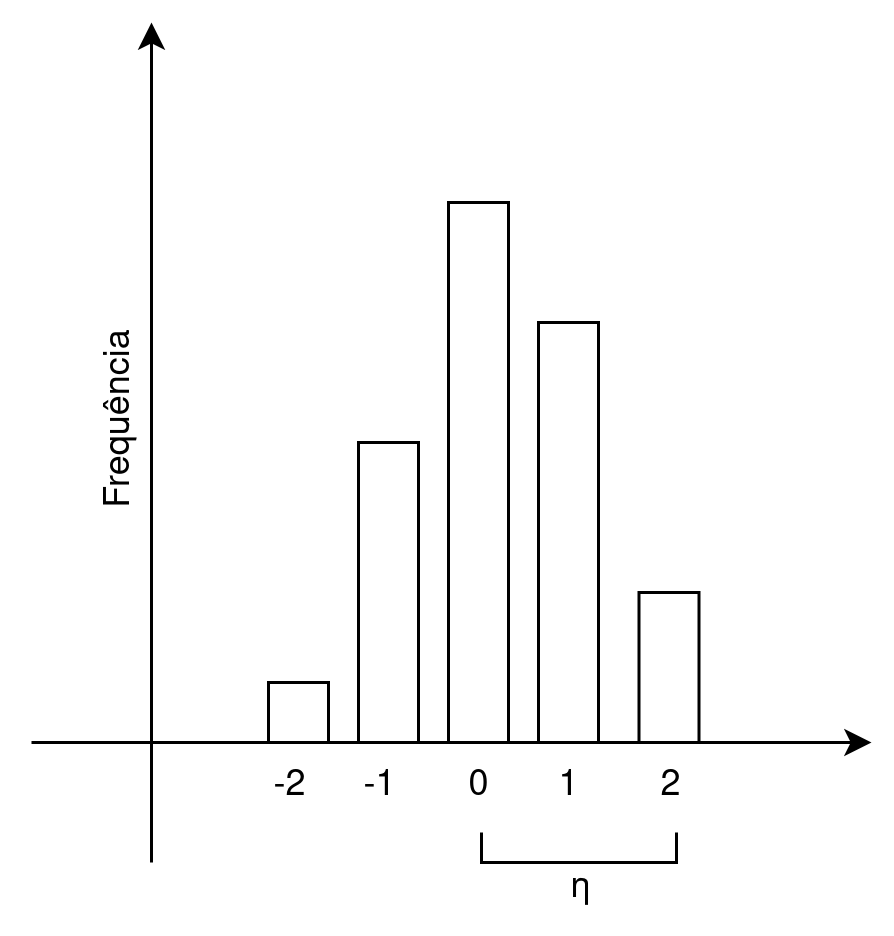
\includegraphics[width=0.65\textwidth]{Figuras/cbd.png}\\
        \footnotesize{Fonte: O autor.}
        \label{fig:cbd}
    \end{figure}

    Como pode ser visto na Figura \ref{fig:kyber_key_gen}, a geração de chaves consiste em gerar quatro matrizes de polinômios, sendo as matrizes \textbf{A} e \textbf{t} as chaves públicas, a matriz \textbf{s} a chave privada e a matriz \textbf{e} apenas uma matriz aleatória de perturbação que pode ser descartada após o final da operação. Perceba que no Algoritmo \ref{algo:kyber_keygen} a ordem das matrizes estão em função do parâmetro k, e seus elementos são polinômios de grau 256 com coeficientes pertencentes ao intervalo ${[}0,3329{]}$. Os elementos da matriz \textbf{A} devem ser gerados o mais aleatório possível, enquanto os elementos das matrizes \textbf{s} e \textbf{e} devem ser gerados por uma distribuição de probabilidade binomial centrada em zero pelo Algoritmo \ref{algo:cbd}. Segundo \cite{kyber}, a motivação para a escolha desta distribuição foi para dificultar alguns ataques conhecidos a esquemas baseados no \ac{LWE}. O Algoritmo \ref{algo:kyber_keygen} representa este processo de geração de chaves.

    \begin{figure}[htb!]
        \centering
        \caption{Ilustração da geração de chaves do K-PKE no modelo matricial.}
        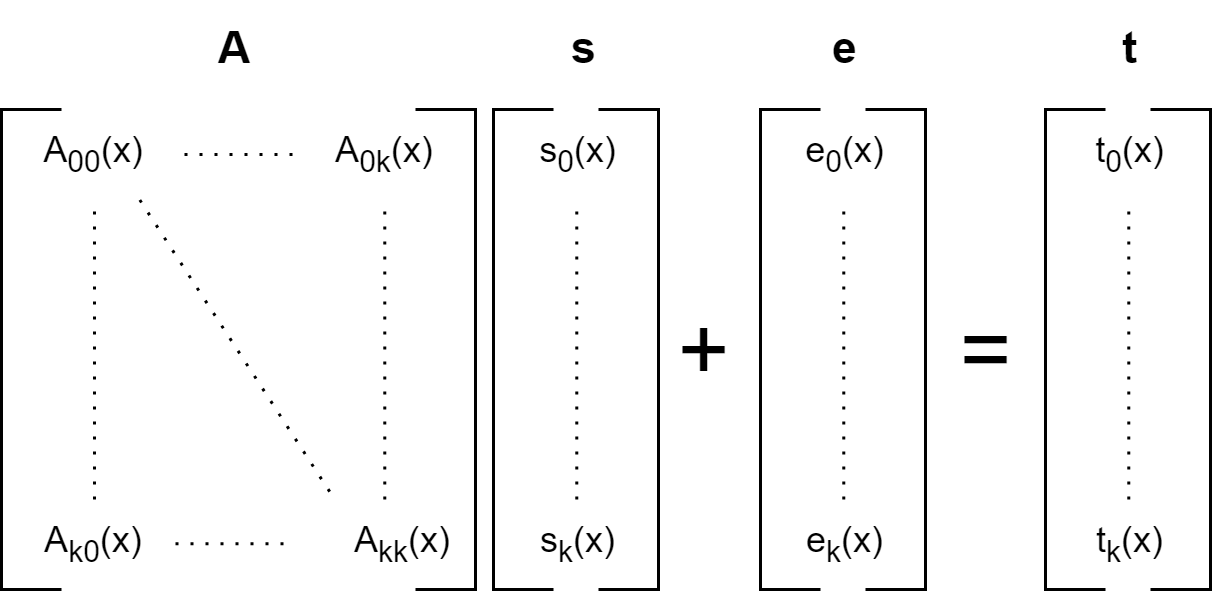
\includegraphics[width=0.75\textwidth]{Figuras/kyber_keygen.png}\\
        \footnotesize{Fonte: O autor.}
        \label{fig:kyber_key_gen}
    \end{figure}

    \begin{algorithm}[!htbp]
        \SetAlgoLined
        \Saida{Chave privada $s \in {[}\mathbb{Z}_{q}{[}x{]}/ \langle x^n + 1 \rangle{]}^k$}
        \Saida{Chave pública $t \in {[}\mathbb{Z}_{q}{[}x{]}/ \langle x^n + 1 \rangle{]}^k$}
        \Saida{Chave pública $A \in {[}\mathbb{Z}_{q}{[}x{]}/ \langle x^n + 1 \rangle{]}^{k \times k}$}
        
        \Para{$i \leftarrow 0$ até $k - 1$}{
            \Para{$j \leftarrow 0$ até $k - 1$}{
                A[i][j] $\leftarrow$ random\_poly()\\
            }
        }

        \Para{$i \leftarrow 0$ até $k - 1$}{
            s[i] $\leftarrow$ random\_poly\_cbd($\eta_1$)\\
        }

        \Para{$i \leftarrow 0$ até $k - 1$}{
            e[i] $\leftarrow$ random\_poly\_cbd($\eta_1$)\\
        }

        $t \leftarrow As + e$\\
        
        \Retorna{s,t,A}
    
        \caption{K-PKE - Geração de chaves}
        \label{algo:kyber_keygen}
    \end{algorithm}

    A cifragem de uma mensagem conforme ilustra a Figura \ref{fig:kyber_enc} consiste na geração de uma matriz \textbf{u} e um polinômio v, isto é, uma mensagem cifrada pelo K-PKE será representada por estes dois elementos. O processo de cifragem de uma mensagem M, representada por um polinômio, consiste em calcular a transposta das chaves públicas \textbf{A} e \textbf{t}, gerar duas matrizes e um polinômio de forma aleatória que seguem a distribuição binomial centrada em zero, e computar a matriz \textbf{u} e o polinômio v como indica o Algoritmo \ref{algo:kyber_encryption}.

    \begin{figure}[htb!]
        \centering
        \caption{Ilustração da cifragem de uma mensagem usando K-PKE no modelo matricial.}
        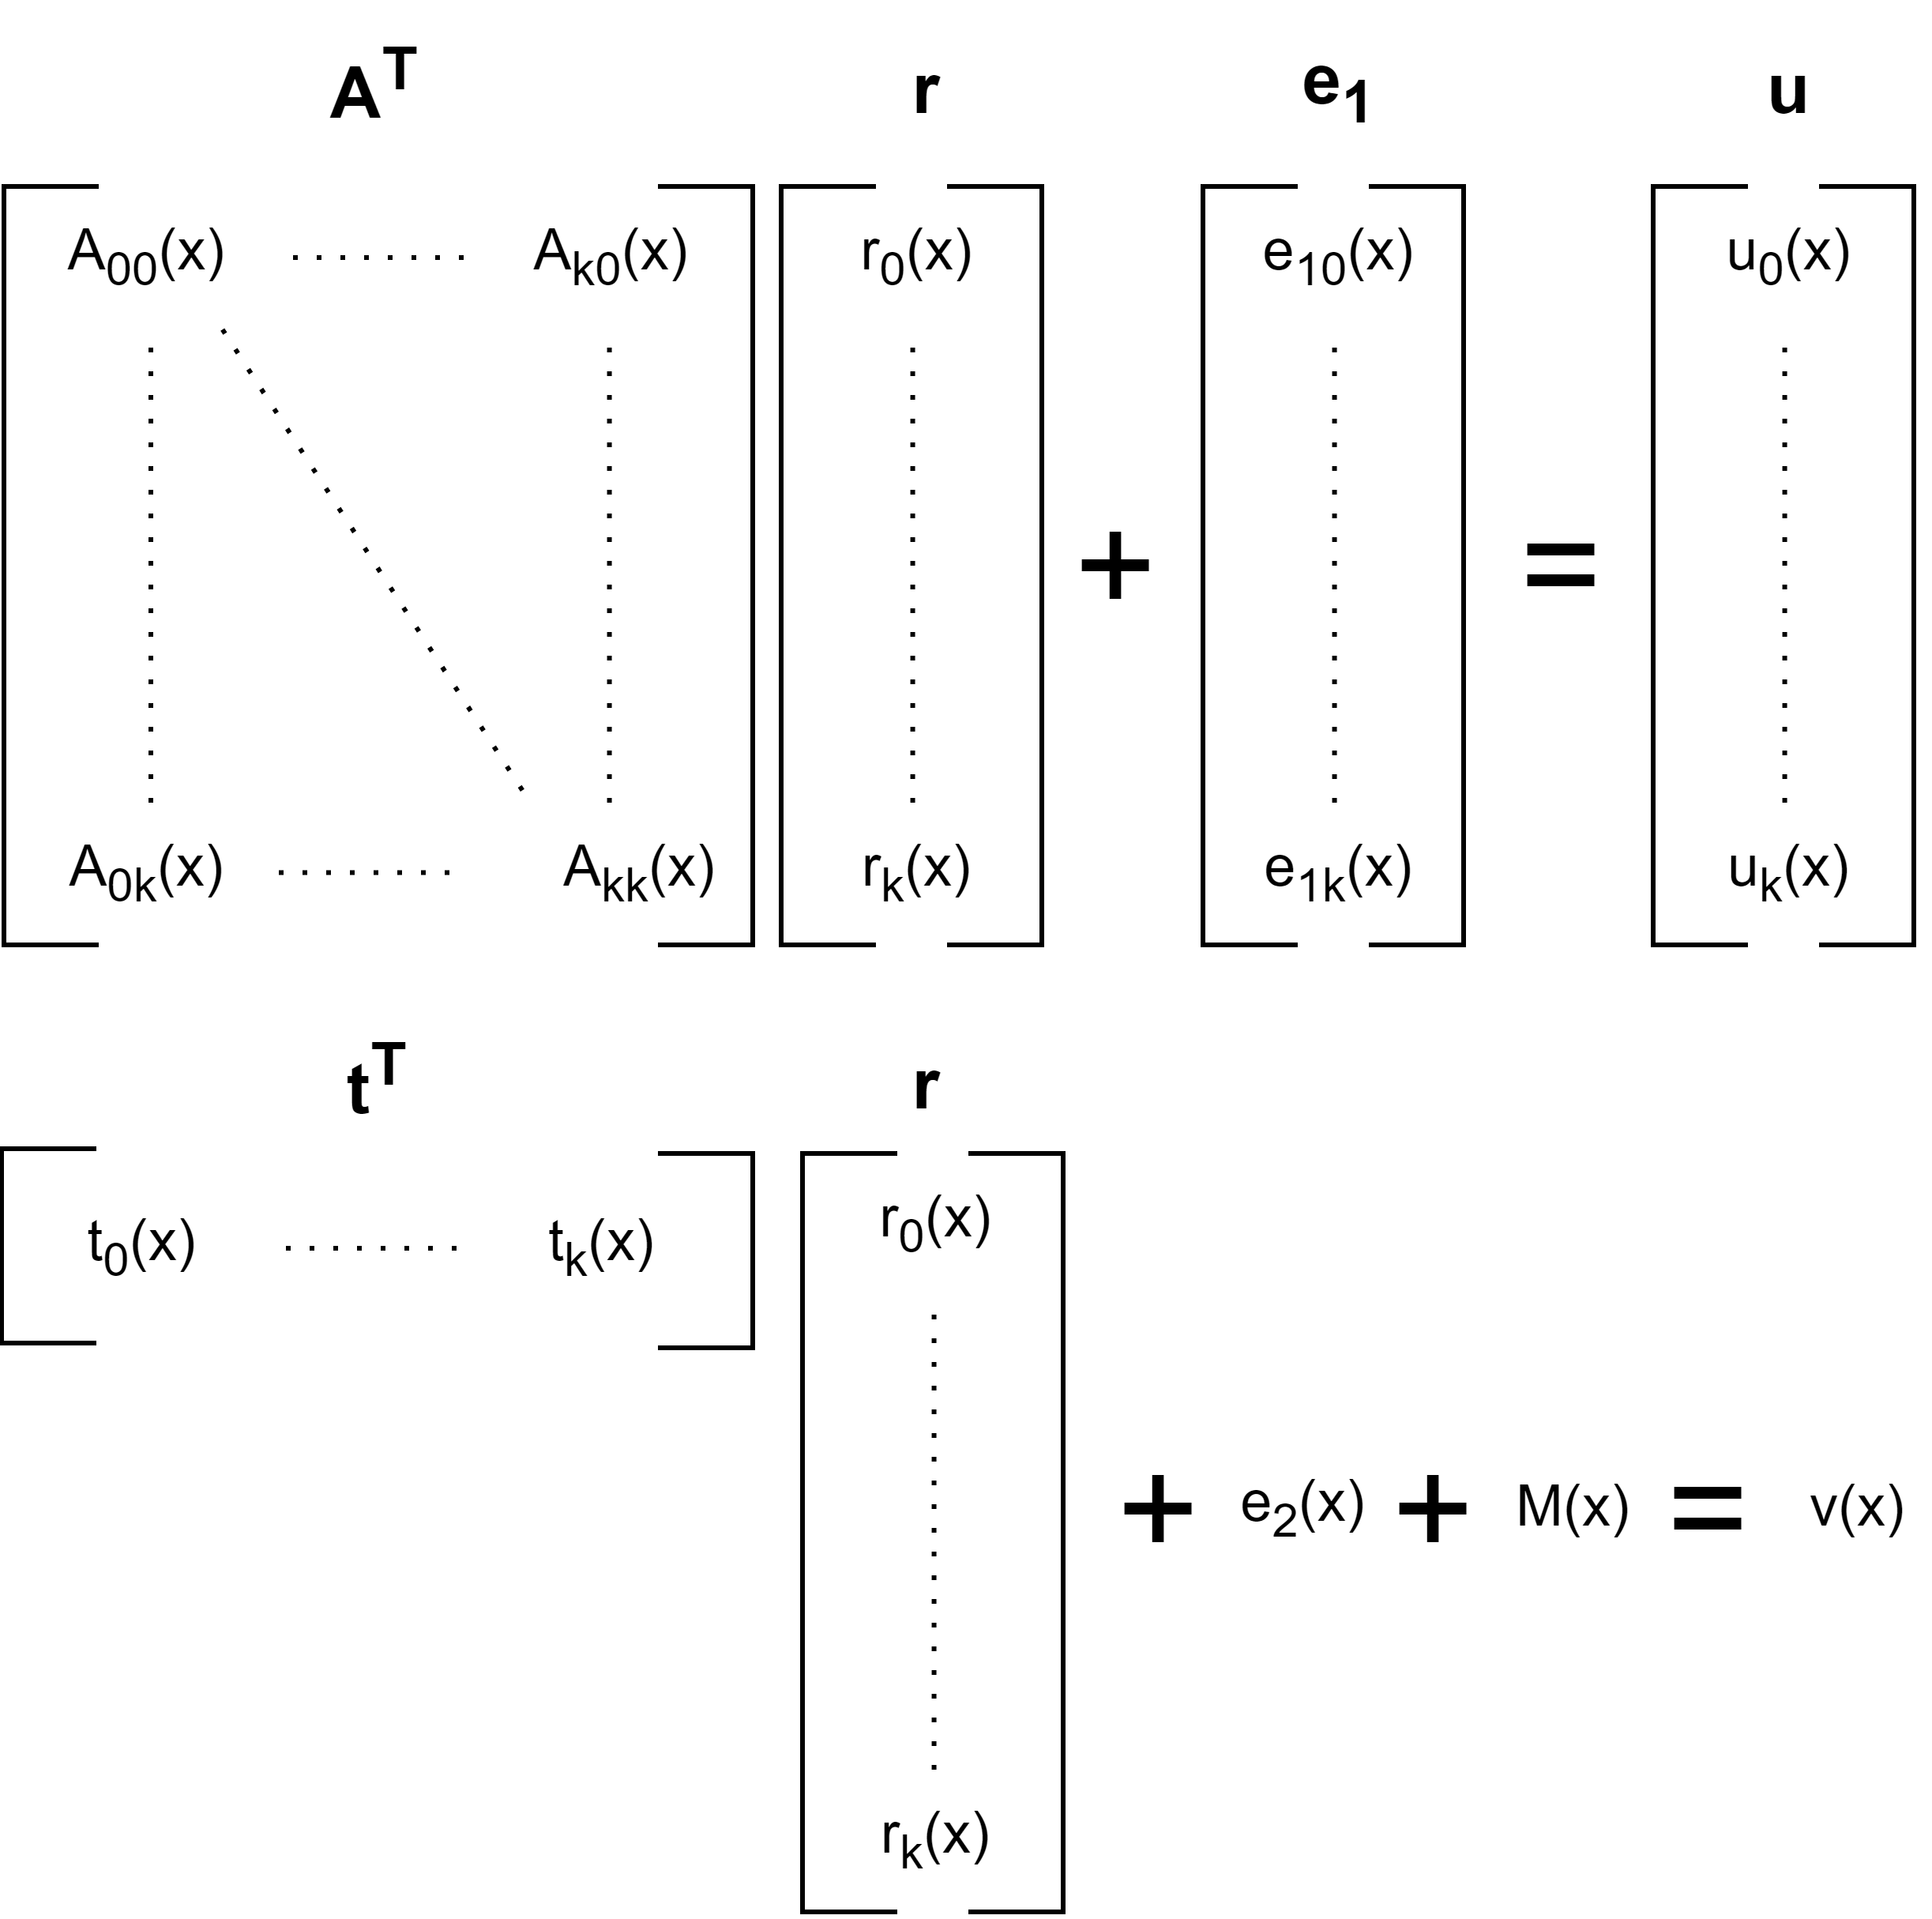
\includegraphics[width=0.75\textwidth]{Figuras/kyber_enc.png}\\         
        \footnotesize{Fonte: O autor.}
        \label{fig:kyber_enc}
    \end{figure}

    \begin{algorithm}[!htbp]
        \SetAlgoLined
        \Entrada{Chave pública A}
        \Entrada{Chave pública t}
        \Entrada{Mensagem m de 32 bytes}
        \Saida{Texto cifrado $u \in {[}\mathbb{Z}_{q}{[}x{]}/ \langle x^n + 1 \rangle{]}^k$}
        \Saida{Texto cifrado $v \in \mathbb{Z}_{q}{[}x{]}/ \langle x^n + 1 \rangle$}
   
        $A^T   \leftarrow CalculaTransposta(A, k)$\\
        $t^{T} \leftarrow CalculaTransposta(t, k)$\\
        
        \Para{$i \leftarrow 0$ até $k - 1$}{
            r[i] $\leftarrow$ random\_poly\_cbd($\eta_1$)\\
        }

        \Para{$i \leftarrow 0$ até $k - 1$}{
            $e_1$[i] $\leftarrow$ random\_poly\_cbd($\eta_2$)\\
        }

        $e_2 \leftarrow$ random\_poly\_cbd($\eta_2$)\\

        $u \leftarrow A^{T} r + e_{1}$\\
        $v \leftarrow t^{T} r + e_{2} + Descomprimir_{q}(m,1)$\\
        
        \Retorna{u,v}
    
        \caption{K-PKE - Cifragem}
        \label{algo:kyber_encryption}
    \end{algorithm}

    A decifragem do K-PKE é relativamente simples, como pode ser visto na Figura \ref{fig:kyber_dec}, basta calcular a transposta da chave privada \textbf{s}, computar $m' = v - s^T u$ e aplicar a função de comprimir em $m'$ conforme o Algoritmo \ref{algo:kyber_decryption}.

    \begin{figure}[htb!]
        \centering
        \caption{Ilustração da decifragem de uma mensagem usando K-PKE no modelo matricial.}
        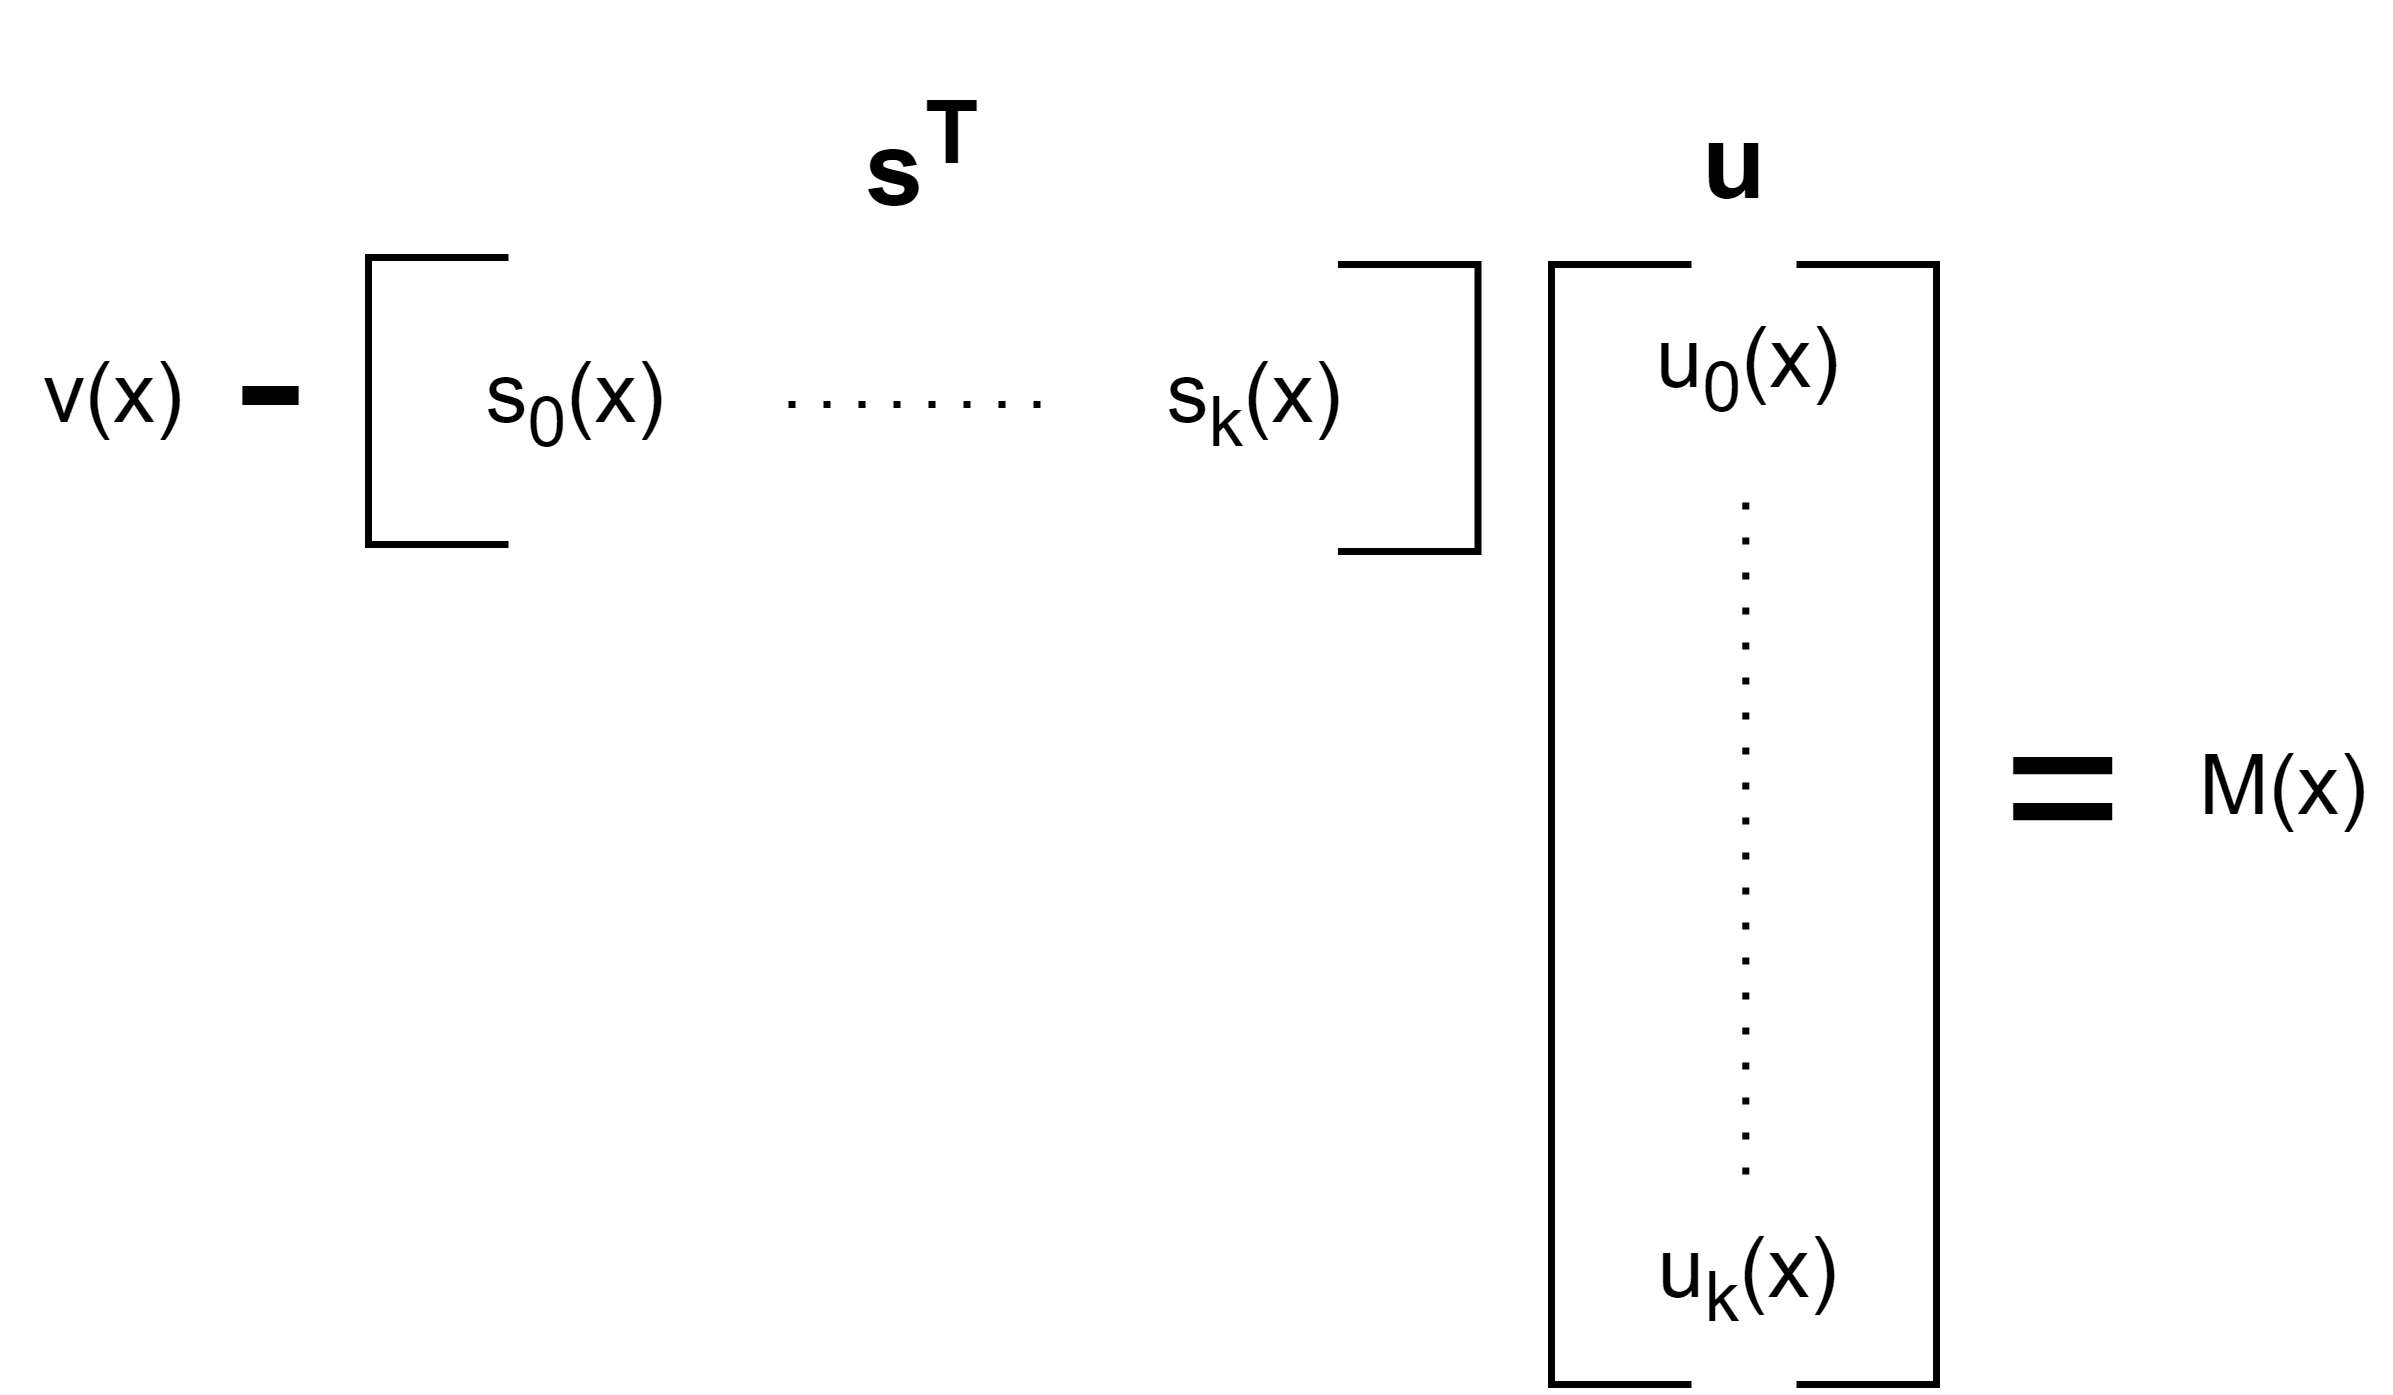
\includegraphics[width=0.65\textwidth]{Figuras/kyber_dec.png}\\
        \footnotesize{Fonte: O autor.}
        \label{fig:kyber_dec}
    \end{figure}

    \begin{algorithm}[!htbp]
            \SetAlgoLined
            \Entrada{Chave privada s}
            \Entrada{Texto cifrado $u \in {[}\mathbb{Z}_{q}{[}x{]}/ \langle x^n + 1 \rangle{]}^k$}
            \Entrada{Texto cifrado $v \in \mathbb{Z}_{q}{[}x{]}/ \langle x^n + 1 \rangle$}
            \Saida{Mensagem m de 32 bytes}
            
            $s^T = CalculaTransposta(s, k)$\\
            $m' = v-s^T u$\\
            $m = Comprimir_{q}(m',1)$
            
            \Retorna{m}
        
            \caption{K-PKE - Decifragem}
            \label{algo:kyber_decryption}
        \end{algorithm}

    Para entender o porquê deste processo de cifragem e decifragem funcionar, observe a seguinte derivação da equação de decifragem do Algoritmo \ref{algo:kyber_decryption}.

    \begin{center}
        $\begin{array}{c}
            v-s^{T}u\\
            (t^{T}r + e_2 + \lceil q/2 \rfloor M) - (s^T(A^T r + e_1))\\
            ((As + e)^T r + e_2 + \lceil q/2 \rfloor M) - (s^T(A^T r + e_1))\\
            ((As)^T r + e^T r + e_2 + \lceil q/2 \rfloor M) - (s^T A^T r + s^T e_1)\\
            (s^T A^T r + e^T r + e_2 + \lceil q/2 \rfloor M) - (s^T A^T r + s^T e_1)\\
            \lceil q/2 \rfloor M + e^T r + e_2 - s^T e_1\\
        \end{array}$
    \end{center}

    Perceba que a função Descomprimir multiplica cada byte da mensagem M(x) por $q / 2$ no processo de cifragem, e depois são adicionados ruídos de norma pequena. Na última linha da derivação temos uma mensagem M com coeficientes grandes adicionado de ruídos com norma pequena, uma vez que foram gerados seguindo uma distribuição de probabilidade centrada em zero. Desta forma é possível remover os ruídos realizando um arredondamento através da função Comprimir.

    Segue um exemplo prático das três etapas do K-PKE com os parâmetros ajustados em $n = 4$, $k = 2$, $q = 3329$, $\eta_1 = 2$ e $\eta_2 = 2$, para simplificar o processo.

    \noindent
    \textbf{Geração de chaves}

        O primeiro passo é gerar a matriz \textbf{A} que será uma das chaves públicas, a matriz \textbf{A} neste caso é uma matriz $2 \times 2$, então é necessário gerar quatro polinômios de grau 3 com coeficientes entre 0 e 3329. Os coeficientes devem ser o mais aleatório possível.
        
        \begin{center}
            \textbf{A} = $\begin{bmatrix}
               2791 + 1035 x + 1916 x^2 + 339 x^3  & 2154 + 2311 x + 517 x^2 + 2496 x^3 \\
               632 + 3048 x + 416 x^2 + 930 x^3  & 1029 + 699 x + 1587 x^2 + 524 x^3
            \end{bmatrix}$
        \end{center}
        

        Para gerar a matriz \textbf{s} e a matriz \textbf{e} é necessário gerar uma matriz coluna $2 \times 1$ com polinômios de grau 3 e com coeficientes entre -2 e 2. Segundo a distribuição binomial centrada em zero, os polinômios de \textbf{s} devem ter mais coeficientes próximos à 0.

        \begin{center}
            \textbf{s} = $\begin{bmatrix}
               -2 x + x^2 + x^3  \\
                1 - 1 x + -2 x^2 - 1 x^3
            \end{bmatrix}$
            %
            \textbf{e} = $\begin{bmatrix}
                1 + 1 x + 2 x^3 \\
                -1 -1 x + 1 x^2 -1 x^3
            \end{bmatrix}$
        \end{center}

        Por fim, para gerar a chave pública \textbf{t}, deve-se computar t = \textbf{A} \textbf{s} + \textbf{e}.

        \begin{center}
             \textbf{t} = $\begin{bmatrix}
                2394 + 1159 x + 105 x^2 + 1857 x^3 \\
                492 + 3023 x + 2948 x^2 + 2686 x^3 
            \end{bmatrix}$   
        \end{center}

        Deve-se ter cuidado ao realizar as operações entre polinômios, pois estes elementos pertencem ao anel quociente $\mathbb{Z}_{3329}[x] / \langle x^4+1 \rangle$. Um exemplo de como trabalhar com as operações de soma, subtração e multiplicação pode ser conferida no Apêndice \ref{ap:abstract_algebra} nos Exemplos \ref{exemplo:soma_em_Z[x]/<I>} e \ref{exemplo:multiplicacao_em_Z[x]/<I>}.

    \noindent
    \textbf{Cifragem}

    Seja M  = 1101 uma mensagem que deseja-se cifrar com K-PKE, representada pelo polinômio M(x) = $1 + 1x + 0 x^2 + 1x^3 = 1+x+x^3$. Primeiro deve-se calcular a transposta das matrizes \textbf{A} e \textbf{t}.

    \begin{center}
       $\textbf{A}^T$ = $\begin{bmatrix}
           2791 + 1035 x + 1916 x^2 + 339 x^3  & 632 + 3048 x + 416 x^2 + 930 x^3 \\
           2154 + 2311 x + 517 x^2 + 2496 x^3  & 1029 + 699 x + 1587 x^2 + 524 x^3
        \end{bmatrix}$

       $\textbf{t}^T$ = $\begin{bmatrix}
           2394 + 1159 x + 105 x^2 + 1857 x^3 & 492 + 3023 x + 2948 x^2 + 2686 x^3 
        \end{bmatrix}$
    \end{center}

    O próximo passo é gerar as matrizes de ruído aleatório \textbf{r} e \textbf{$e_1$}, e o polinômio de ruído \textbf{$e_2$}.

    \begin{center}
        \textbf{r} = $\begin{bmatrix}
           -1 + x + x^2 + 2 x^3 \\
            1 + x^3
        \end{bmatrix}$
        %
        $\textbf{e}_1$ = $\begin{bmatrix}
            1 + x + x^2 \\
            -1 -x + x^2 -x^3
        \end{bmatrix}$
        %
        $e_2(x) = -x^2 + x^3$
    \end{center}

    A cifragem de uma mensagem M(x) gera dois elementos, uma matriz \textbf{u} e um polinômio v(x). A geração da matriz \textbf{u} é obtida computando $\textbf{A}^T \textbf{r} + \textbf{e}_1$, o resultado desta operação segue abaixo. 

    
    \begin{center}
        \textbf{u} = $\begin{bmatrix}
            246 + 218 x + 719 x^2 + 3098 x^3 \\
            527 + 2082 x + 20 x^2 + 2863 x^3
        \end{bmatrix}$
    \end{center}

    Antes de realizar o cálculo de v(x) é preciso aplicar a função Descomprimir a mensagem M(x), que consiste em multiplicar cada coeficiente da mensagem M(x) por $q/2^d$ e arredondar para o inteiro mais próximo. Segundo a documentação do \ac{NIST} os parâmetros q e d da função Descomprimir são respectivamente 3329 e 1. Desta forma, a mensagem M(x) passa a ser $M(x) = 1665 + 1665x + 1665 x^3$. Com isso, para obtermos o último elemento da mensagem cifrada, o polinômio v(x), deve-se computar $\textbf{t}^T$ \textbf{r} + $e_2$(x) + M(x).

    \begin{center}
        $v(x) = 2447 + 908 x + 3323 x^2 + 2381 x^3$
    \end{center}

    \noindent
    \textbf{Decifragem}

    Para realizar a decifragem de \textbf{u} e v(x), é necessário calcular a transposta da chave privada \textbf{s} e computar $m'(x) = v - \textbf{s}^T u$, após computado $m'(x)$ deve-se aplicar a função Comprimir a ela para realizar o arredondamento, assim obtendo a mensagem original M(x). 

    \begin{center}
            $\textbf{s}^T$ = $\begin{bmatrix}
               -2 x + x^2 + x^3 & 1 - 1 x + -2 x^2 - 1 x^3
            \end{bmatrix}$
    \end{center}
    
    \begin{center}
            $m'(x) = 2447 + 908 x + 3323 x^2 + 2381 x^3 -$
            
            $\begin{bmatrix}
               -2 x + x^2 + x^3 & 1 - 1 x + -2 x^2 - 1 x^3
            \end{bmatrix}$
            %
            $\begin{bmatrix}
            246 + 218 x + 719 x^2 + 3098 x^3 \\
            527 + 2082 x + 20 x^2 + 2863 x^3
        \end{bmatrix}$
    \end{center}

    \begin{center}
        $m'(x) = 1663 + 1245 x + 206 x^2 + 1874 x^3$
    \end{center}

    Aplicando a função Comprimir em m'(x), obtemos a mensagem original M, finalizando o processo de decifragem do K-PKE.

    \begin{center}
        $M(x) = 1 + 1 x + 0 x^2 + 1 x^3$ \\
        $M = 1101$
    \end{center}
    
    %https://link.springer.com/chapter/10.1007/978-981-19-7644-5_4
    %https://www.youtube.com/watch?v=94fdZvSx-NY&t=429s ******** IMPORTANTE  *********
    %https://asecuritysite.com/encryption/lwe3

\section{Encapsulamento de chaves ML-KEM}
\label{sec:ml-kem}
    O \ac{ML-KEM} é um algoritmo de encapsulamento de chave, ou seja, como dito na Seção \ref{sec:kem}, os algoritmos de encapsulamento de chave têm como objetivo estabelecer uma chave simétrica aleatória em comum entre duas partes. A principal diferença entre o \ac{ML-KEM} e o K-PKE, está na mensagem cifrada, enquanto o K-PKE permite cifrar uma mensagem qualquer, o \ac{ML-KEM} determina a mensagem cifrada, esta mensagem é a chave simétrica compartilhada. A nomenclatura de alguns termos também é diferente, as chaves públicas são chamadas de chaves de encapsulamento, a chave privada é dita de desencapsulamento.

    O funcionamento do \ac{ML-KEM} é semelhante ao K-PKE, entretanto a forma como essa comunicação deve ocorrer é pré-estabelecida, e deve seguir o diagrama da Figura \ref{fig:kem_nist} segundo o \ac{NIST}. Perceba que não são cifradas e decifradas mensagens quaisquer como no K-PKE. Em vez disso, o algoritmo gera esta mensagem que é a chave simétrica compartilhada de forma aleatória. A razão disso se dá pelo fato do \ac{ML-KEM} ser um algoritmo de encapsulamento de chave, este abordado no Capítulo \ref{cap:criptografia}.

    \begin{figure}[htb!]
        \centering
        \caption{Estabelecimento de uma chave compartilhada com o \ac{ML-KEM}.}
        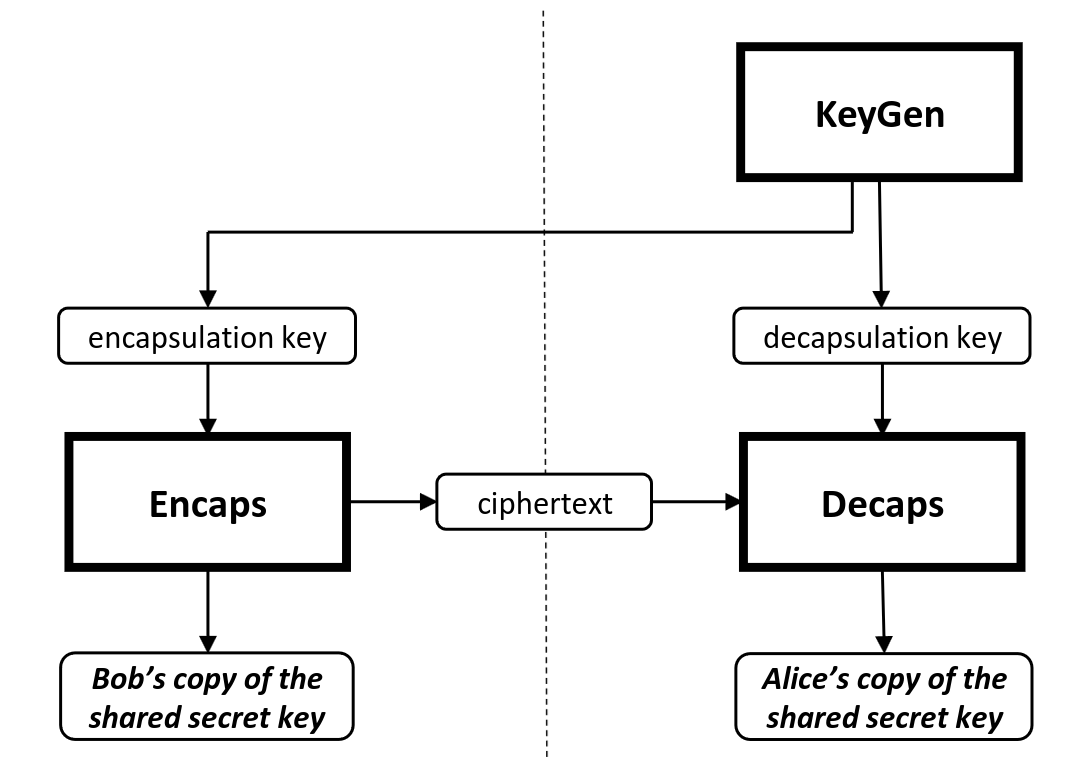
\includegraphics[width=0.75\textwidth]{Figuras/kem_nist.png}\\
        \footnotesize{Fonte: \cite{kyber}.}
        \label{fig:kem_nist}
    \end{figure}

    \begin{algorithm}[!htbp]
            \SetAlgoLined
            \Saida{Chave de desencapsulamento $dk\_pke\_s \in {[}\mathbb{Z}_{q}{[}x{]}/ \langle x^n + 1 \rangle{]}^k$}
            \Saida{Chave de encapsulamento $ek\_pke\_t \in {[}\mathbb{Z}_{q}{[}x{]}/ \langle x^n + 1 \rangle{]}^k$}
            \Saida{Chave de encapsulamento $ek\_pke\_a \in {[}\mathbb{Z}_{q}{[}x{]}/ \langle x^n + 1 \rangle{]}^{k \times k}$}
            
            k\_pke\_s, k\_pke\_t, k\_pke\_a $\leftarrow$ k\_pke\_keygen()\\
            dk\_pke\_s $\leftarrow$ k\_pke\_s\\
            ek\_pke\_t $\leftarrow$ k\_pke\_t\\
            ek\_pke\_a $\leftarrow$ k\_pke\_a
            
            \Retorna{dk\_pke\_s, ek\_pke\_t, ek\_pke\_a}
        
            \caption{ML-KEM - Geração de chaves}
            \label{algo:ml_kem_keygen}
        \end{algorithm}

        No modelo simplificado da geração de chaves do \ac{ML-KEM}, descrito pelo Algoritmo \ref{algo:ml_kem_keygen}, a geração de chaves é idêntica à geração de chaves do K-PKE, com apenas algumas renomeações nas chaves criptográficas, em que dk\_pke\_s é a chave privada de desencapsulamento, ek\_pke\_t e ek\_pke\_a são as chaves públicas de encapsulamento.
        
        \begin{algorithm}[!htbp]
            \SetAlgoLined
            \Entrada{Chave de encapsulamento $ek\_pke\_t \in {[}\mathbb{Z}_{q}{[}x{]}/ \langle x^n + 1 \rangle{]}^k$}
            \Entrada{Chave de encapsulamento $ek\_pke\_a \in {[}\mathbb{Z}_{q}{[}x{]}/ \langle x^n + 1 \rangle{]}^{k \times k}$}
            \Saida{Chave compartilhada cifrada $c\_u \in {[}\mathbb{Z}_{q}{[}x{]}/ \langle x^n + 1 \rangle{]}^k$}
            \Saida{Chave compartilhada cifrada $c\_v \in {[}\mathbb{Z}_{q}{[}x{]}/ \langle x^n + 1 \rangle{]}^k$}
            \Saida{Chave compartilhada $K \in \mathbb{Z}_{q}{[}x{]}/ \langle x^n + 1 \rangle$}
       
            K $\leftarrow$ random\_poly()\\
            c\_u, c\_v $\leftarrow$ k\_pke\_cifragem(ek\_pke\_a, ek\_pke\_t, K)

            \Retorna{c\_u, c\_v, K}
            
            \caption{ML-KEM - Encapsulamento}
            \label{algo:ml_kem_encapsulation}
        \end{algorithm}

        O algoritmo de encapsulamento gera uma chave privada aleatória K, que será a chave compartilhada. A chave compartilhada K é cifrada pela chave de encapsulamento
        
        \begin{algorithm}[!htbp]
            \SetAlgoLined
            \Entrada{Chave compartilhada cifrada $c\_u \in {[}\mathbb{Z}_{q}{[}x{]}/ \langle x^n + 1 \rangle{]}^k$}
            \Entrada{Chave compartilhada cifrada $c\_v \in {[}\mathbb{Z}_{q}{[}x{]}/ \langle x^n + 1 \rangle{]}^k$}
            \Entrada{Chave de desencapsulamento $dk\_pke\_s \in {[}\mathbb{Z}_{q}{[}x{]}/ \langle x^n + 1 \rangle{]}^k$}
            \Saida{Chave compartilhada $K \in \mathbb{Z}_{q}{[}x{]}/ \langle x^n + 1 \rangle$}
            
            $K \leftarrow$ k\_pke\_decifragem(c\_u, c\_v, dk\_pke\_s)
            
            \Retorna{K}
        
            \caption{ML-KEM - Desencapsulamento}
            \label{algo:ml_kem_decapsulation}
        \end{algorithm}

        A implementação na linguagem C dos algoritmos \ref{algo:ml_kem_keygen}, \ref{algo:ml_kem_encapsulation} e \ref{algo:ml_kem_decapsulation} pode ser encontrada no repositório do GitHub em \url{https://github.com/opallace/ML-KEM}, e também outras ferramentas de teste e \textit{benchmark}. Este repositório conta com uma implementação fiel dos algoritmos deste capítulo, e também com um manual de uso e exemplos básicos de códigos para facilitar o uso por terceiros. É importante lembrar que os algoritmos apresentados neste trabalho e implementados no repositório não devem serem utilizados em ambientes reais. Estes foram desenvolvidos e simplificados para fins acadêmicos. 

\section{Parâmetros}
\label{sec:parametros}
    Os parâmetros estabelecidos para o \ac{ML-KEM} constam na FIPS 203 do \ac{NIST} em \cite{kyber}. São fornecidos parâmetros para 3 modelos do \ac{ML-KEM} com relação ao seu nível de segurança: ML-KEM-512, ML-KEM-768 e ML-KEM-1024. A Tabela \ref{tab:kyber_param} mostra os parâmetros para estes três modelos.\\ 
    
    \begin{table}[h!]
        \centering
        \caption{Parâmetros do \ac{ML-KEM}.}
        \begin{tabular}{|c|c|c|c|c|c|c|c|c|}
        \hline
                  & $n$ & $k$ & $q$ & $\eta_1$ & $\eta_2$ & $\delta$ & \ac{NIST} \textit{Level Security} \\ \hline
        ML-KEM-512  & 256 & 2 & 3329 & 3 & 2 & $2^{-139}$ & I   \\ \hline
        ML-KEM-768  & 256 & 3 & 3329 & 2 & 2 & $2^{-169}$ & III \\ \hline
        ML-KEM-1024 & 256 & 4 & 3329 & 2 & 2 & $2^{-174}$ & V   \\ \hline
        \end{tabular}\\
        \footnotesize{Fonte: O autor.}
        \label{tab:kyber_param}
    \end{table}

    O parâmetro $\delta$ é a probabilidade de erro no processo de decifragem. Os níveis de segurança do \ac{NIST} vão de I a V, em que os níveis I, III e V significam ser pelo menos tão difícil de quebrar quanto o AES128, AES192 e AES256, respectivamente, através do método de busca exaustiva da chave.

    Para alterar estes parâmetros na implementação do GitHub basta modificar os valores definidos no arquivo params.h e recompilar todo o projeto. Os exemplos de geração de chaves, cifragem e decifragem demonstrados na Seção \ref{sec:k-pke} utilizaram os parâmetros $n = 4$, $k = 2$, $q = 3329$, $\eta_1 = 2$ e $\eta_2 = 2$ a fim de simplificar os cálculos envolvidos. Entretanto, devido ao parâmetro $q$ estar diretamente relacionado com a taxa de sucesso no processo de decifragem, foi escolhido não modificar. 
    
\section{Segurança}
    A segurança do \ac{ML-KEM} está diretamente relacionada com a dificuldade de se resolver o problema \ac{MLWE}, abordado no Capítulo \ref{cap:lattice_problems}. Ou seja, encontrar um algoritmo que fornecidos as chaves públicas \textbf{A} e \textbf{t}, encontre a chave privada \textbf{s} com alta probabilidade. Segundo \cite{kyber2}, o \ac{ML-KEM} é considerado seguro para todos os ataques clássicos e quânticos conhecidos, para os parâmetros estabelecidos na Tabela \ref{tab:kyber_param}.

\section{Desempenho}
    O \ac{ML-KEM} destaca-se em tempo de geração de chaves, encapsulamento e desencapsulamento comparado a outros algoritmos de encapsulamento de chaves do programa \ac{NIST} \ac{PQC}, como pode ser visto na Figura \ref{fig:benchmark}. 

    \begin{figure}[htb!]
        \centering
        \caption{Comparação de desempenho entre os algoritmos de encapsulamento no programa \ac{NIST} \ac{PQC}.}
        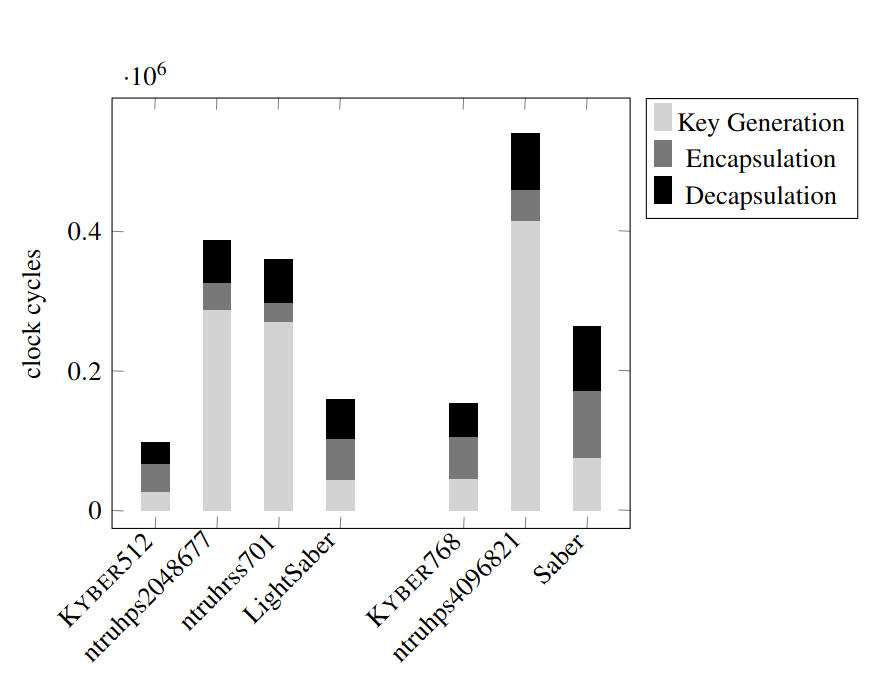
\includegraphics[width=0.75\textwidth]{Figuras/benchmark.png}\\
        \footnotesize{Fonte: Adaptado de \cite{nist_round_3_report}.}
        \label{fig:benchmark}
    \end{figure}
    
    Isso se deve ao fato dos seus cálculos necessitarem principalmente de soma e multiplicação de matrizes e polinômios, que são operações de baixa complexidade. A soma de matrizes e polinômios, por exemplo, possui complexidade $\mathcal{O}(n)$ e a multiplicação matricial $\mathcal{O}(n^2)$. Pelo fato das matrizes serem pequenas, $2 \times 2$, $3 \times 3$ ou $4 \times 4$, dependendo do parâmetro k escolhido, a complexidade do algoritmo em geral é mais afetada pela multiplicação dos elementos dessas matrizes, que no caso são polinômios, e das primitivas criptográficas utilizadas durante os processos (estas primitivas foram removidas deste trabalho para sua simplificação). A multiplicação dos polinômios, pelo fato de pertencerem a um anel quociente, podem ser otimizadas pelo método \ac{NTT}, possuindo assim complexidade logarítmica ao invés de quadrática. Estes fatores de otimização contribuíram significativamente para seu desempenho, e em sua seleção para padronização.
\chapter{Conclusão}
\label{cap:consideracoes_parciais}
    O algoritmo de criptografia \ac{ML-KEM} é relevante para manter a segurança dos dados em um futuro onde a computação quântica terá capacidade computacional para quebrar a segurança dos principais algoritmos de criptografia atuais. Em 2016, foi publicado o algoritmo Kyber no programa \ac{PQC} do \ac{NIST}, com o objetivo de ser o principal algoritmo de criptografia de chave pública, este foi escolhido e padronizado em 2023 e renomeado para \ac{ML-KEM}. O \ac{ML-KEM} possui sua segurança baseada na dificuldade de se resolver o problema \ac{MLWE} \cite{module-lwe}. O fato deste problema ser recente implica na carência de materiais de fácil compreensão sobre o assunto, tendo em sua maioria artigos que exigem um alto nível de conhecimento para se compreender. Esta foi uma das dificuldades na elaboração deste trabalho, além da necessidade de conhecimento em diversas áreas como álgebra abstrata, teoria dos números, espaços métricos, álgebra linear e criptologia. 

    Dentre os objetivos específicos propostos no Capítulo 1, a implementação simplificada do algoritmo \ac{ML-KEM}, desenvolvida neste trabalho, fornece uma base para que o leitor possa compreender o funcionamento deste algoritmo, e também, a partir deste, possa desenvolver por conta um modelo mais próximo da versão oficial que envolvem conceitos mais sofisticados de segurança e otimização.

    Os trabalhos futuros que podem ter como base este documento incluem um aprofundamento nos problemas computacionais baseados em reticulados, além de otimizações utilizadas nas operações do \ac{ML-KEM} como \ac{NTT}. Outro conceito recente de criptografia é a criptografia homomórfica, este possui estudos que utilizam variantes do problema \ac{LWE}.

\newpage

\bibliographystyle{pkg/abnt-alf}
\bibliography{bibliografia}

\appendix
% ----------------------------------------------------------
% Apêndices
% ----------------------------------------------------------

\chapter{Conceitos matemáticos}
\label{ap:conceitos_matematicos}

Neste capítulo iremos abordar alguns conceitos matemáticos importantes para o entendimento deste trabalho.

\section{Aritmética modular}
    A aritmética modular é um dos conceitos estudados pelo ramo da matemática conhecido como teoria dos números, que será amplamente utilizado neste trabalho. O conhecimento de aritmética modular será necessário para compreender alguns problemas de criptografia abordados nos Capítulo \ref{cap:criptografia} e \ref{cap:lattice_problems}. O algoritmo \ac{ML-KEM} também faz o uso da aritmética modular nas operações aritméticas entre polinômios, na qual é vista com mais detalhes no Apêndice \ref{ap:abstract_algebra}.

\begin{definition}[divisibilidade]
 Sejam $a$ e $b$ inteiros diferentes de $0$, é dito que $a$ é divisível por $b$ se e somente se existe um inteiro $c$ tal que $a = b.c$, a notação usada para denotar essa divisibilidade de $a$ por $b$ é $a\:|\:b$.
 \end{definition}

\begin{theorem}
    Se $a\:|\:b$ e $a\:|\:c$, então $(b + c)\:|\:a$.
\end{theorem}

\begin{theorem}
    Se $a\:|\:b$, então $(a.c)\:|\:b$.
\end{theorem}

\begin{theorem}
    Se $a\:|\:b$ e $b\:|\:c$, então $a\:|\:c$.
\end{theorem}

\begin{theorem}
Seja $n \in \mathbb{Z}$ e $d \in \mathbb{Z}_{+}$, existe um único par de inteiros $q$ e $r$ com $0 \leq r < d$ tais que $n = d.q + r$.
\end{theorem}

Sejam $n,d,q,r \in \mathbb{Z}$ tais que $d > 0$, $n = d.q + r$ e $0 \leq r < d$, definem-se as funções \textbf{div} e \textbf{mod} tais que:

\begin{itemize}
	\item $n$\ \textbf{div} $d = q$;
	\item $n$\ \textbf{mod} $d = r$.
\end{itemize}

\begin{definition}[Congruência modular]
Dados $j, k \in \mathbb{Z}$ e $m \in \mathbb{Z}_{+}$, é dito que $j$ é congruente a $k$ no módulo $m$ se e somente se $(j - k) \ |\  m$. A notação de congruência é $j \equiv k\ (\textbf{mod}\ m)$, ou seja, $j$ e $k$ são o mesmo número no módulo m.
\end{definition}

    \noindent
    \textbf{Propriedades da congruência modular}:
    \begin{itemize}
         \item \textbf{Propriedade reflexiva:} Seja $m \in \mathbb{Z}_{+}$, $n \equiv n\: (\textbf{mod}\: m)\: \forall n \in \mathbb{Z}$;
    	\item \textbf{Propriedade simétrica:} Seja $m \in \mathbb{Z}_{+}$, $j \equiv k\: (\textbf{mod}\: m)$ se e somente se $k \equiv j\: (\textbf{mod}\: m)$;
    	\item \textbf{Propriedade transitiva:} Seja $m \in \mathbb{Z}_{+}$, se $j \equiv k\: (\textbf{mod}\: m)$ e $k \equiv i\: (\textbf{mod}\: m)$ então $j \equiv i\: (\textbf{mod}\: m)$.
    \end{itemize}
    
    \begin{exemplo}
    para facilitar o entendimento sobre conceito de congruência, considere um relógio de 12 horas. Se agora são 5 horas, que horas serão daqui a 10 horas? Como este relógio não possui 15 horas, reinicia-se a contagem a partir de 0 quando o relógio chega em 12 horas. Dessa forma tem-se que 15 = 12 + 3; neste caso, se agora são 5 horas, daqui a 10 horas serão 3 horas. Desta forma é dito que $15 \equiv 3\ (\textbf{mod}\ 12)$, visto que $(15 - 3)\ |\ 12$.
    \qed
    \end{exemplo}

\pagebreak
\section{Teoria dos números}

    Esta seção apresenta alguns conceitos estudados no campo da teoria dos números mencionados na Seção \ref{sec:problemas_computacionais}, onde é abordado os problemas que os algoritmos de criptografia atuais são baseados.

    \begin{definition}[número primo]
        Um número natural maior que 1 que possui como divisores positivos apenas 1 e ele próprio.
    \end{definition}

    \begin{definition}[coprimos]
        Dois números são coprimos, ou primos entre si, se o único divisor comum entre eles for o número 1.
    \end{definition}

    \begin{exemplo}
        os divisores do número 4 são: 2 e 1, e os divisores do número 9 são: 3 e 1. Portando os números 4 e 9 são coprimos.
    \qed
    \end{exemplo}
   

    \begin{definition}[número composto]
        Dado $n,n_1,n_2 \in \mathbb{N}$ tal que $n > 1$, $n\ |\ n_1$ e $n\ |\ n_2$. Temos que $n$ é dito composto se $n = n_1 n_2$, com $1 < n_1 < n$ e $1 < n_1 < n$. 
    \end{definition}

    \begin{theorem}[teorema fundamental da aritmética]
        Todo número natural maior que 1 ou é primo, ou pode ser escrito como um produto de números primos.
    \end{theorem}

    Segundo o teorema fundamental da aritmética dado um número composto, por exemplo o número 145, podemos representá-lo pela multiplicação de números primos, neste caso 5 e 29. O problema da fatoração prima, abordado na Seção \ref{sec:problema_fatoracao_prima} utiliza este teorema.

    \begin{definition}[ordem multiplicativa]
        Dado os números inteiros positivos $n$ e $m$, tais que $n$ e $m$ são coprimos, a ordem multiplicativa de $n$ módulo $m$ é o menor valor inteiro positivo $k$ que satisfaz $n^k \equiv 1\ (\textbf{mod}\ m)$.
    \end{definition}

    \begin{exemplo}
        tem-se que \(2^6 \equiv 1\ (\textbf{mod}\ 7)\). No entanto, \(2^3 \equiv 1\ (\textbf{mod}\ 7)\). Observa-se que ambos satisfazem a congruência; porém, 3 é o menor expoente que satisfaz a equação. Portanto, conclui-se que 3 é a ordem multiplicativa de 2 módulo 7.
    \qed
    \end{exemplo}

    \begin{definition}[função totiente de Euler]
        A função totiente de Euler de um número natural $n$, denotada por $\varphi(n)$, é a quantidade de números coprimos a $n$ no intervalo $1 \le \varphi(n) < n$.
    \end{definition}

    \begin{exemplo}
         tem-se $\varphi(10) = 4$ pois a quantidade de números coprimos a 10 no intervalo ${[}1,10{[}$ é o conjunto $\{1, 3, 7, 9\}$ contendo 4 elementos.
    \qed
    \end{exemplo}

    \begin{definition}[raiz primitiva módulo m]
        Se a ordem multiplicativa de $k$ módulo $m$ é igual à função totiente de Euler para $m$, dizemos que $k$ é uma raiz primitiva módulo $m$.
    \end{definition}

    \begin{exemplo}
        é dito que 3 é uma raiz primitiva módulo 10, visto que a ordem multiplicativa de 3 e 10 é 4, e como calculado anteriormente, $\varphi(10) = 4$. Sendo assim, como a ordem multiplicativa entre 3 e 10 é igual à função totiente de 10, o número 3 é uma raiz primitiva módulo 10. Este conceito é utilizado no problema do logaritmo discreto, abordado na Seção \ref{sec:problema_logaritmo_discreto}.
    \qed
    \end{exemplo}

\pagebreak
\section{Álgebra linear}
Esta seção se dedica a alguns conceitos de álgebra linear essenciais para a compreensão deste trabalho. A álgebra linear é um ramo da matemática que se dedica no estudo de equações lineares, vetores, espaços vetoriais, matrizes, entre outros.

\begin{definition}[matriz]
    Chamamos de matriz $m \times n$ uma tabela de elementos dispostos em m linhas e n colunas.
\end{definition}

    \begin{center}
        $\textbf{A}_{m \times n} = \begin{bmatrix}
            a_{11} & a_{12} & . & . & . & b_{1n}\\
            a_{21} & a_{22} & . & . & . & b_{2n}\\
            a_{31} & a_{32} & . & . & . & b_{3n}\\
            .      & .      & . &   &   & .     \\
            .      & .      &   & . &   & .     \\
            .      & .      &   &   & . & .     \\
            a_{m1} & a_{m2} &   &   &   & a_{mn}
        \end{bmatrix}$
        %
        $= {[}a_{ij}{]}_{m \times n}$
    \end{center}

    O número de linhas e colunas é dito a ordem de uma matriz. É importante ressaltar algumas matrizes especiais, como a matriz quadrada, em que o número de linhas é igual o número de colunas; matriz nula, em que todos os elementos são zero, tal matriz é representada por \textbf{0}; matriz coluna, em que se tem apenas uma coluna e analogamente matriz linha, em que se tem apenas uma linha; por fim, matriz identidade quadrada, denotada por \textbf{I} tal que $a_{ii} = 1$ e $a_{ij} = 0$ para $i \neq j$.

    A seguir, é definida as operações e propriedades de soma entre matrizes de mesma ordem, multiplicação de uma matriz por um escalar, operação de transposição e multiplicação entre matrizes.
    
    A adição de matrizes de mesma ordem, isto é $\textbf{A}_{m \times n}$ + $\textbf{B}_{m \times n}$ é representada por:

                        $$\textbf{A} + \textbf{B} = {[}a_{ij} + b_{ij}{]}_{m \times n}$$
                
    \noindent
    e apresenta as seguintes propriedades:
    \begin{itemize}
        \item[(i)] $\textbf{A} + \textbf{B} = \textbf{B} + \textbf{A}$,
        \item[(ii)] $\textbf{A} + (\textbf{B} + \textbf{C}) = (\textbf{A} + \textbf{B}) + \textbf{C}$,
        \item[(iii)] $\textbf{A} + \textbf{0} = \textbf{A}$, onde \textbf{0} representa matriz nula.
    \end{itemize}

    A multiplicação de um escalar $k$ por uma matriz $\textbf{A} = {[}a_{ij}{]}_{m \times n}$ é representada por:

                            $$k.\textbf{A} = {[}k a_{ij}{]}_{m \times n}$$

    \noindent
    e segue as seguintes propriedades, dadas duas matrizes \textbf{A} e \textbf{B} de mesma ordem e $k,k_1$ e $k_2$ escalares:
     \begin{itemize}
        \item[(i)] $k(\textbf{A} + \textbf{B}) = k\textbf{A} + k\textbf{B}$,
        \item[(ii)] $(k_1 + k_2)\textbf{A} = k_1 \textbf{A} + k_2 \textbf{A}$,
        \item[(iii)] $0.\textbf{A} = \textbf{0}$, neste caso, se multiplicarmos o escalar zero, obtemos a matriz nula,
        \item[(iv)] $k_1(k_2 \textbf{A}) = (k_1 k_2)\textbf{A}$.
    \end{itemize}

    Outra operação importante é a de transposição, seja a matriz $\textbf{A} = {[}a_{ij}{]}_{m \times n}$, sua transposta, denotada $\textbf{A}^T = {[}b_{ij}{]}_{n \times m}$, é tal que $b_{ij} = a_{ji}$. 
    
    \begin{center}
        $\textbf{A} = \begin{bmatrix}
           2  & 1 \\
           0  & 3 \\
           -1 & 4
        \end{bmatrix}_{3 \times 2}$
        %
        $\textbf{A}^T = \begin{bmatrix}
           2 & 0 & -1 \\
           1 & 3 & 4
        \end{bmatrix}_{2 \times 3}$
    \end{center}

    A operação de transposição respeita as seguintes propriedades:
    \begin{itemize}
        \item[(i)] $(\textbf{A}^T)^T = \textbf{A}$,
        \item[(ii)] $(\textbf{A} + \textbf{B})^T = \textbf{A}^T + \textbf{B}^T$,
        \item[(iii)] $(\textbf{AB})^T = \textbf{B}^T \textbf{A}^T$,
        \item[(iv)] $(k \textbf{A})^T = k \textbf{A}^T$, onde $k$ é um escalar.
    \end{itemize}

    A operação de multiplicação entre matrizes é um pouco mais complexa e só pode ser efetuada se o número de colunas da primeira matriz for igual ao número de linhas da segunda, isto é, sejam as matrizes $\textbf{A} = {[}a_{ij}{]}_{m \times n}$ e $\textbf{B} = {[}b_{rs}{]}_{n \times p}$, definimos a operação $\textbf{AB} = {[}c_{uv}{]}_{m \times p}$, onde

                     $$c_{uv} = \sum_{k=1}^{n} a_{uk} b_{kv}$$

    \noindent
    e respeita as seguintes propriedades:
    \begin{itemize}
        \item[(i)] $\textbf{AB} \neq \textbf{BA}$,
        \item[(ii)] $\textbf{AI} = \textbf{IA} = \textbf{A}$,
        \item[(iii)] $\textbf{A}(\textbf{B} + \textbf{C}) = \textbf{AB} + \textbf{AC}$,
        \item [(iv)] $(\textbf{A} + \textbf{B})\textbf{C} = \textbf{AC} + \textbf{BC}$,
        \item [(v)] $(\textbf{AB})\textbf{C} = \textbf{A}(\textbf{BC})$,
        \item [(vi)] $(\textbf{AB})^T = \textbf{B}^T \textbf{A}^T$,
        \item [(vii)] $\textbf{0}.\textbf{A} = \textbf{0}$ e $\textbf{A}.\textbf{0} = \textbf{0}$, e \textbf{0} representa a matriz nula.
    \end{itemize}

\begin{definition}[vetores]
    Dado um segmento de reta orientado AB, um vetor é o conjunto de todos os segmentos orientados equipolentes\footnote{Dois segmentos são equipolentes quanto têm a mesma direção, o mesmo sentido e o mesmo comprimento. A relação de equipolência é denotada por $\sim$} a AB.
\end{definition}

Seja $\vec{v}$ este conjunto, podemos escrever que $\vec{v} = \{XY\ |\ XY \sim AB\}$, onde XY é um segmento qualquer do conjunto. O vetor representante desse conjunto inicia na origem.

\begin{definition}[vetor nulo]
    Dizemos que um vetor é nulo quando sua origem e a extremidade coincidem. Denotamos esse vetor por $\vec{0}$.
\end{definition}

\begin{definition}[espaços vetoriais]
    Um espaço vetorial é um conjunto $V$ de vetores, não vazio, com duas operações: soma entre dois vetores $\vec{u},\vec{v} \in V$ que resulta em $\vec{v} + \vec{u} \in V$, e multiplicação entre um vetor $\vec{v} \in V$ por escalar $a \in \mathbb{R}$, cujo resultado é $a\vec{v} \in V$. Tais que para quaisquer $\vec{u},\vec{v},\vec{w} \in V$ e $a,b \in \mathbb{R}$, os seguintes axiomas são satisfeitos:
    
    \noindent
    \textbf{Adição}:
    \begin{itemize}
        \item[(i)] $(\vec{u} + \vec{v}) + \vec{w} = \vec{u} + (\vec{v} + \vec{w})$,
        \item[(ii)] $\vec{u} + \vec{v} = \vec{v} + \vec{u}$,
        \item[(iii)] Existe $\vec{0} \in V$ tal que $\vec{u} + \vec{0} = \vec{u}$ e
        \item[(iv)] Existe $-\vec{u} \in V$ tal que $\vec{u} + (-\vec{u}) = \vec{0}$.
    \end{itemize}
    
    \noindent
    \textbf{Multiplicação por escalar}:
    \begin{itemize}
        \item[(i)] $a(\vec{u} + \vec{v}) = a\vec{u} + a\vec{v}$,
        \item[(ii)] $(a + b)\vec{v} = a\vec{v} + b\vec{v}$,
        \item[(iii)] $(ab)\vec{v} = a(b\vec{v})$ e
        \item[(iv)] $1\vec{u} = \vec{u}$.
    \end{itemize}
\end{definition}

    \begin{exemplo}
    \label{exemplo:espaco_vetorial_rn}
        Seja um espaço vetorial o conjunto de vetores $V = \mathbb{R}^{n} = \{(x_1, x_2, ... , x_n)\ |\ x_i \in \mathbb{R}\}$.
    \qed
    \end{exemplo}

    \begin{exemplo}
    \label{exemplo:espaco_vetorial_matriz}
        $V = M(m,n)$, o conjunto das matrizes reais $m \times n$.
    \qed
    \end{exemplo}

    \begin{exemplo}
    \label{exemplo:espaco_vetorial_polinomio}
        Tem-se também o espaço vetorial $V = P_n = \{a_0 + a_1 x + a_2 x^2 + ... + a_n x^n\ |\ a_i \in \mathbb{R}\}$ definido por todos os polinômios com coeficientes reais de grau menor ou igual a $n$.
    \qed
    \end{exemplo}
    
    Os elementos dos conjuntos dos exemplos \ref{exemplo:espaco_vetorial_rn},\ref{exemplo:espaco_vetorial_matriz} e \ref{exemplo:espaco_vetorial_polinomio} respeitam todas as propriedades de um espaço vetorial, portanto são espaços vetoriais.

\begin{definition}[produto interno]
    Seja $V$ um espaço vetorial sobre $\mathbb{R}$. O produto interno é definido por $\langle .,. \rangle : V \times V \rightarrow \mathbb{R}$, onde tal operação satisfaz as seguintes propriedades:

    \begin{itemize}
        \item[(i)] $\langle \vec{v},\vec{v} \rangle \ge 0$ para todo vetor $\vec{v}$, e\\ $\langle \vec{v},\vec{v} \rangle = 0$ se, e somente se $\vec{v} = \vec{0}$;
        \item[(ii)] $\langle a\vec{v}_1,\vec{v}_2 \rangle = a\langle \vec{v}_1,\vec{v}_2 \rangle$ para todo $a \in \mathbb{R}$;
        \item[(iii)] $\langle \vec{v}_1 + \vec{v}_2,\vec{v}_3 \rangle = \langle \vec{v}_1,\vec{v}_3 \rangle + \langle \vec{v}_2,\vec{v}_3 \rangle$;
        \item[(iv)] $\langle \vec{v}_1,\vec{v}_2 \rangle = \langle \vec{v}_2,\vec{v}_1 \rangle$.
    \end{itemize}
    
\end{definition}

    Sejam os vetores $\vec{a} = (a_1,a_2,a_3,...,a_n)$ e $\vec{b} = (b_1,b_2,b_3,...,b_n)$, o produto interno entre $\vec{a}$ e $\vec{b}$ é dado por $\langle \vec{a}, \vec{b} \rangle = a_1 b_1 + a_2 b_2 + a_3 b_3 + ... + a_n b_n$.\\

    Em um espaço vetorial com produto interno definido, podemos realizar outras operações entre vetores como calcular a norma vetorial, ângulo e a projeção entre dois vetores.

\begin{definition}[ortogonalidade entre vetores]
    Dois vetores $\vec{u}$, $\vec{v}$ são ditos ortogonais se o ângulo entre eles for de $90^{\circ}$, em outras palavras, quando o produto interno $\langle \vec{u}, \vec{v} \rangle = 0$, denota-se tal ortogonalidade por $\vec{u} \perp \vec{v}$.
\end{definition}

\begin{definition}[norma vetorial]
    Norma consiste em uma função que associa um vetor do espaço vetorial em um número real não negativo. A norma de um vetor está associada ao seu comprimento, também denominada como módulo de um vetor.
\end{definition}

    Neste trabalho iremos fazer o uso apenas da norma euclidiana. Seja o vetor $\vec{v} = (a_1,a_2,...,a_n)$, sua norma euclidiana é definida por: $$\lVert \vec{v} \rVert = \sqrt{a_{1}^2 + a_{2}^2 + ... + a_{n}^2}$$

\begin{definition}[projeção entre vetores]
A projeção vetorial de um vetor $\vec{u}$ sobre um vetor não nulo $\vec{v}$, denotado por $proj_{\vec{v}}\Vec{u}$, é uma projeção ortogonal de $\vec{u}$ sobre uma reta paralela à $\vec{v}$.
\end{definition}

    Sejam os vetores $\vec{u}$ e $\vec{v}$, para calcular o vetor projeção $\vec{w}$ de $\vec{u}$ sobre $\vec{v}$, como mostra a Figura \ref{fig:projecao}, utiliza-se a fórmula: $$ \vec{w} = proj_{\vec{v}}\Vec{u} = \frac{\langle\vec{u}, \Vec{v}\rangle}{\lVert \Vec{v} \rVert^{2}}\Vec{v} $$

    \begin{figure}[htb!]
        \centering
        \caption{Projeção de $\vec{u}$ sobre $\vec{v}$.}
        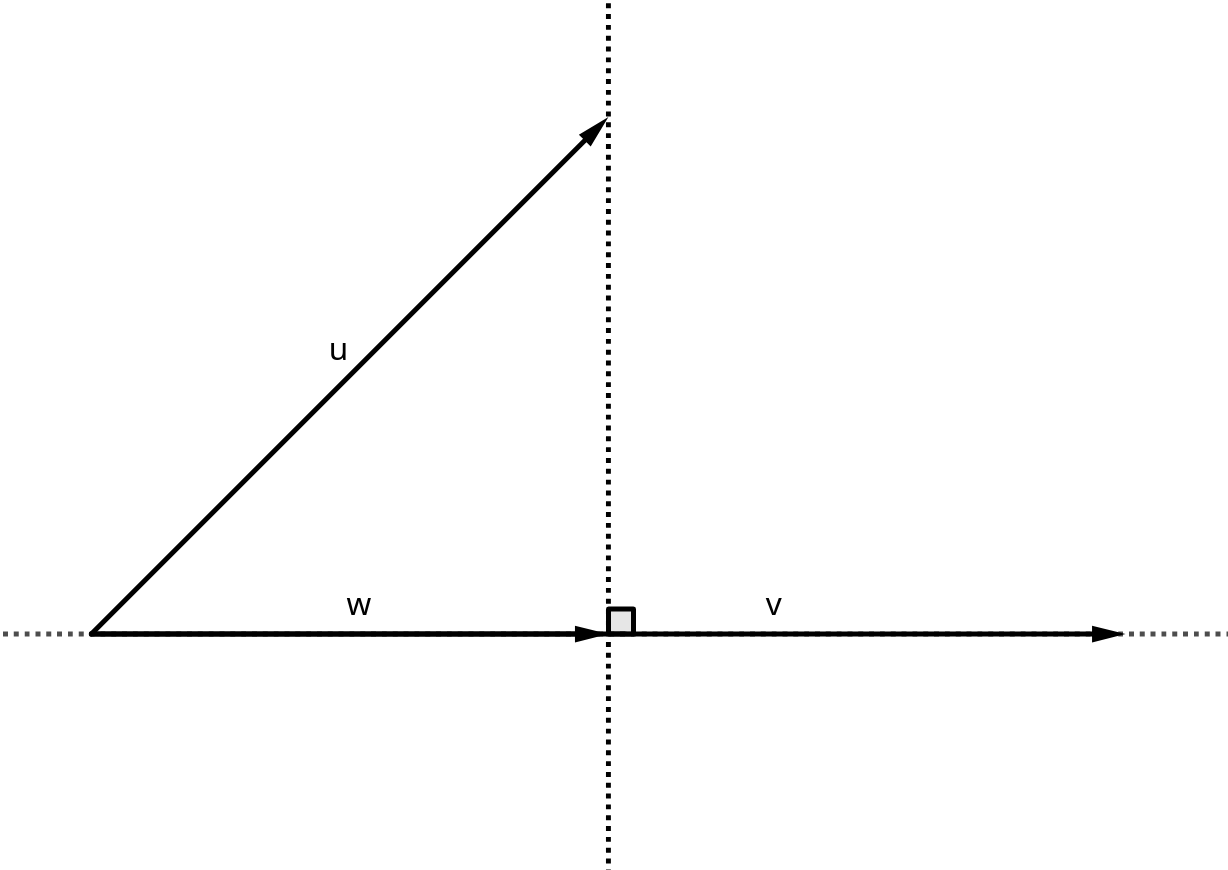
\includegraphics[width=0.75\textwidth]{Figuras/projecao.png}\\
        \footnotesize{Fonte: O autor.}
        \label{fig:projecao}
    \end{figure}

\begin{definition}[combinação linear]
    Seja $V$ um espaço vetorial, dizemos que um vetor $\vec{v}$ é uma combinação linear de outros vetores $\vec{v_1}, \vec{v_2}, \vec{v_3},...,\vec{v_n} \in V$ se e somente se existem escalares $a_1, a_2, a_3,...,a_n \in \mathbb{R}$ tais que $\vec{v}=a_1 \vec{v_1}+a_2 \vec{v_2}+ a_3 \vec{v_3}+...+a_n \vec{v_n}$.
\end{definition}

    \begin{exemplo}
        O vetor $\vec{w} = (5,3) \in \mathbb{R}^{2}$, pode ser escrito como uma combinação linear dos vetores $\vec{u} = (1,0)$ e $\vec{v} = (0,1)$. Isso pode ser visto por $(5,3) = 5(1,0) + 3(0,1)$.
    \qed
    \end{exemplo}

\begin{definition}[dependência e independência linear]
    Seja $V$ um espaço vetorial qualquer e $\vec{v_1}, \vec{v_2}, \vec{v_3},...,\vec{v_n} \in V$, dizemos que o conjunto $\{ \vec{v_1}, \vec{v_2}, \vec{v_3},...,\vec{v_n} \}$ é linearmente independente quando a combinação linear nula $\vec{0}=a_1 \vec{v_1}+a_2 \vec{v_2}+ a_3 \vec{v_3}+...+a_n \vec{v_n}$ implicar que obrigatoriamente $a_1=a_2=a_3=...=a_n= 0$. Caso exista algum escalar $a_n \neq 0$ que satisfaça a combinação linear nula, dizemos que o conjunto $\{ \vec{v_1}, \vec{v_2}, \vec{v_3},...,\vec{v_n} \}$ é linearmente dependente.
\end{definition}

    \begin{exemplo}
        os vetores $\vec{u} = (1,0)$ e $\vec{u} = (0,1)$ são linearmente independentes pois\\

        \begin{center}
            $\begin{array}{rl}
                a_1 (1,0) + a_2 (0,1) &= (0,0)\\
                (a_1,0) + (0,a_2) &= (0,0)\\
                (a_1,a_2) &= (0,0)\\
                a_1 &= 0\\ 
                a_2 &= 0
            \end{array}$
        \end{center}

    \qed
    \end{exemplo}
    
    \begin{exemplo}
        Seja os vetores $\vec{u} = (1,2)$ e $\vec{u} = (3,6)$ do espaço vetorial $\mathbb{R}^{2}$, tais vetores não são linearmente independentes pois,
    
        \begin{center}
            $\begin{array}{rl}
                a_1 (1,2) + a_2 (3,6) &= (0,0)\\
                (a_1,2 a_1) + (3 a_2, 6 a_2) &= (0,0)\\
                (a_1 + 3 a_2, 2 a_1 + 6 a_2) &= (0,0)\\
            \end{array}$
        \end{center}
        
        \begin{center}
            $\begin{cases}
                a_1 + 3 a_2   &= 0\\
                2 a_1 + 6 a_2 &= 0
            \end{cases}$
        \end{center}
    
        \noindent
        resolvendo o sistema acima, encontramos infinitas soluções em que $a_1$ e $a_2$ são diferentes de 0, determinando assim que os vetores $\vec{u} = (1,2)$ e $\vec{u} = (3,6)$ são linearmente dependentes.
    
    \qed
    \end{exemplo}
    
\begin{definition}[base de espaços vetoriais]
    Um conjunto de vetores $\beta = \{ \vec{v_1}, \vec{v_2}, \vec{v_3},...,\vec{v_n} \}$ é considerado uma base para um espaço vetorial $V$, se as seguintes condições forem satisfeitas:
    \begin{itemize}
        \item[(i)] $\beta$ é linearmente independente;
        \item[(ii)] para todo vetor $\vec{v}\in V$ existem $a_1, a_2, \ldots, a_n\in \mathbb{R}$ tal que $\vec{v}=a_1\vec{v_1}+a_2\vec{v_2}+\ldots+a_n\vec{v_n}$.
    \end{itemize}
\end{definition}

\begin{definition}[dimensão de espaços vetoriais]
    A dimensão de um espaço vetorial $V$ é a quantidade de elementos de sua base geradora, denotada por $Dim(V)$.
\end{definition}

\pagebreak
\section{Álgebra abstrata}
\label{ap:abstract_algebra}
Uma operação binária interna é uma função (eventualmente) parcial $\oplus:\mathbb{A}^{2}\rightarrow\mathbb{A}$ e é usualmente denotada como um par ordenado <$\mathbb{A}, \oplus$>, no qual $\mathbb{A}$ é denominado conjunto suporte. A seguir são apresentadas algumas propriedades de operações binárias internas.

\begin{itemize}
    \item[(i)] \textbf{fechada:} $\oplus:\mathbb{A}^{2}\rightarrow\mathbb{A}$ é função total
	\item[(ii)] \textbf{comutativa:} $\forall a,b \in \mathbb{A}\:(a \oplus b = b \oplus a)$
	\item[(iii)] \textbf{associativa:} $\forall a,b \in \mathbb{A}\:((a \oplus b) \oplus c = (c \oplus b) \oplus a = a \oplus b \oplus c)$
	\item[(iv)] \textbf{elemento neutro:} $\exists e \in \mathbb{A}\:\forall a \in \mathbb{A}\:(a \oplus e = a = e \oplus a)$
	\item[(v)] \textbf{elemento inverso:} $\forall a \in \mathbb{A}\:\exists \bar{a} \in \mathbb{A}\:(a \oplus \bar{a} = e = \bar{a} \oplus a)$
\end{itemize}

\begin{definition}[grupoide]
    Um grupoide é um conjunto não vazio junto a uma operação binária fechada. Se um grupoide respeitar a propriedade de comutatividade, denomina-se grupoide abeliano.
\end{definition}

    \begin{exemplo}
         a realização da operação de subtração entre os elementos do conjunto dos inteiros é sempre um inteiro, portanto ($\mathbb{Z},-$) denota um grupoide não abeliano, visto que se $a,b \in \mathbb{Z}\ a - b \neq b - a$. 
    \qed
    \end{exemplo}

\begin{definition}[semigrupo]
    Um semigrupo é definido como um conjunto não vazio que possui uma operação binária fechada e associativa. Se a operação binária também respeitar a propriedade de comutatividade, é dito que o semigrupo é abeliano.
\end{definition}

\begin{definition}[monoide]
    Os monoides são definidos por um conjunto não vazio e uma operação binária que respeita as propriedades de fechamento, associatividade e possui elemento neutro. Se um monoide também possuir a propriedade de comutatividade, é dito que o monoide é abeliano.
\end{definition}

    \begin{exemplo}
         A realização da operação de multiplicação entre os elementos do conjunto $\mathbb{Z}^{*}$ denotam um semigrupo, visto que respeitam a associatividade, portanto ($\mathbb{Z}^{*},*$) é um semigrupo. Entretanto, a estrutura ($\mathbb{Z}^{*},*$) também pode ser classificada como um monoide, pois possui elemento neutro 1 para a operação de multiplicação.
    \qed
    \end{exemplo}
    
    
\begin{definition}[grupo]
    Grupos são definidos como um  conjunto não vazio que possui operação binária que respeita as propriedades de fechamento, associatividade, possui elemento neutro e elemento inverso. Se um grupo respeitar a propriedade de comutatividade, é dito que o grupo é abeliano.
\end{definition}

    \begin{exemplo}
    \label{exemplo:grupo}
        A estrutura ($\mathbb{Z},+$) é um grupo, visto que a operação de soma entre os elementos de $\mathbb{Z}$ possui as propriedades de fechamento, associatividade, possui elemento neutro 0 e possui elemento inverso $a,a' \in \mathbb{Z}\ a + (-a) = 0$. A estrutura ($\mathbb{Z},+$) também possui a propriedade comutativa, sendo assim, classificada como um grupo abeliano. 
    \qed
    \end{exemplo}
    
\begin{definition}[anel]
    Um anel ($A, \oplus, \otimes$) é uma álgebra constituída de um conjunto suporte e duas operações $\oplus$ e $\otimes$ na qual:

    \begin{itemize}
        \item ($A , \oplus$) é um grupo abeliano;
    	\item $\otimes$ é associativo; e
    	\item $\forall a,b,c \in A (a \otimes (b \oplus c)) = ((a \otimes b) \oplus (a \otimes c))$.
    \end{itemize}
\end{definition}

    \begin{exemplo}
        A estrutura ($\mathbb{Z},+,*$) é um anel, pois demonstramos no exemplo \ref{exemplo:grupo} que a estrutura ($\mathbb{Z},+$) é um grupo abeliano, a operação de multiplicação é associativa entre os elementos de $\mathbb{Z}$ e também respeita a distributividade da multiplicação na soma.
    \qed
    \end{exemplo}

    Outros anéis importantes que serão utilizados com frequência neste trabalho são: anel polinomial e anel quociente.
    
\begin{definition}[anel polinomial]
    Sendo o polinômio P na forma $P(x) = a_0 + a_1x^1 + a_2x^2 + ... + a_nx^n$ com $n \in \mathbb{N}$, P é um anel polinomial se seus coeficientes ($a_0, a_1, a_2,...,a_n$) pertencem a um anel A. Denota-se então que $P \in A[x]$.
\end{definition}

\begin{definition}[anel quociente]
    Seja um anel $A$ e um ideal bilateral $I \subseteq A$. Tem-se o anel quociente $A/I$ formado pelo conjunto de todas as classes de equivalência modulo $I$.
\end{definition}

\begin{definition}[classes e relações de equivalência]
    Uma relação $R$ sobre dois elementos $x,y \in A$ denotada por $xRy$, é uma relação de equivalência se satisfazer as seguintes propriedades:

    \begin{itemize}
        \item[(i)] reflexiva: $xRx$
        \item[(ii)] simétrica: $xRy$ então, $yRx$
        \item[(iii)] transitiva: $xRy$ e $yRz$ então $xRz$
    \end{itemize}

    O conjunto de todos os elementos pertencentes a uma relação de equivalência $R$, é conhecido como classe de equivalência de $R$.
\end{definition}

\begin{definition}[ideais]
    Sejam $A$ um anel e $I$ um subconjunto não vazio de $A$.
    Dizemos que $I$ é um ideal à esquerda de $A$ se satisfazer as seguintes propriedades:
    
    \begin{enumerate}
        \item[(i)] se $x, y,  \in I$, então $x-y \in I$ e,
        \item[(ii)] se $a \in A, x \in I$, então $ax \in I$.
    \end{enumerate}
    
    Analogamente define-se um ideal à direita I de $A$ como um subconjunto não vazio tal que:
    
    \begin{enumerate}
        \item[(i)] se $x, y,  \in I$, então $x-y \in I$ e,
        \item[(ii)] se $a \in A, x \in I$, então $xa \in I$.
    \end{enumerate}
    
    Se $I$ é um ideal simultaneamente à direita e à esquerda de $R$ dizemos que $I$ é um ideal (bilateral) de $R$.
\end{definition}

    \begin{exemplo}
         Sendo o anel dos inteiros $\mathbb{Z}$ e o conjunto dos inteiros pares representado por $2\mathbb{Z} \subset \mathbb{Z}$ é um ideal de $\mathbb{Z}$, pois a subtração de qualquer inteiro par por outro inteiro par resulta em um inteiro par, e a multiplicação de um inteiro par por outro inteiro qualquer, resulta em um inteiro par. 
    \qed
    \end{exemplo}

    Outro tipo ideal que deve ser mencionado, é o ideal polinomial na forma $\langle x^{n} + 1 \rangle \subset \mathbb{Z}[x]$. Este ideal representa todos os polinômios múltiplos de $x^{n} + 1$ pertencentes a $\mathbb{Z}[x]$, visto que, sejam $P(x),Q(x) \in \langle x^{n} + 1 \rangle $, $P(x)(x^{n}+1) - Q(x)(x^{n}+1) = (P(x)-Q(x))(x^{n}+1)$ e seja $G(x) \notin \langle x^{n} + 1 \rangle$, $P(x)(x^{n}+1)G(x) = (P(x)G(x))(x^{n}+1)$.

    O anel quociente $\mathbb{Z}_p[x] / \langle x^n+1 \rangle$ é de grande importância para esse trabalho, esta estrutura é utilizada no esquema M-LWE empregado pelo Kyber. Seja $a,b \in \mathbb{Z}_p[x]$, um ideal $\langle x^n+1 \rangle \in \mathbb{Z}_p[x]$ e a relação de equivalência definida por $a \equiv b\ (\textbf{mod}\ \langle x^n+1 \rangle$) se $a - b \in \langle x^n+1 \rangle$. O anel quociente $\mathbb{Z}_p[x] / \langle x^n+1 \rangle$ é uma classe de equivalência formada pelo conjunto de todos os polinômios pertencentes a $\mathbb{Z}_p[x]$ módulo $x^n+1$. Isto é, um polinômio pertencente a $\mathbb{Z}_p[x] / \langle x^n+1 \rangle$ é um polinômio que pertence ao anel $\mathbb{Z}_p[x]$ de grau menor que $n$ com coeficientes entre 0 e $p-1$.

    \begin{exemplo}
    \label{exemplo:soma_em_Z[x]/<I>}
        seja o anel quociente $\mathbb{Z}_7[x] / \langle x^5+1 \rangle$ e os polinômios $a(x) = 5 + 6x + x^3 - 2x^4 - 3x^5 \in \mathbb{Z}_7[x] / \langle x^5+1 \rangle$ e $b(x) = 1 - x + 4x^2 + 3x^4 + x^5 \in \mathbb{Z}_7[x] / \langle x^5+1 \rangle$. A operação de soma entre $a(x)$ e $b(x)$ é definida por:

        \begin{center}
            $\begin{array}{rl}
                c(x) &= a(x) + b(x)\\
                c(x) &= (5 + 6x + x^3 - 2x^4 - 3x^5) + (1 - x + 4x^2 + 3x^4 + x^5)\\
                c(x) &= 6 + 5x + 4x^2 + x^3 + x^4 - 2x^5
            \end{array}$
        \end{center}
    \qed
    \end{exemplo}

    A operação de soma não altera o grau do polinômio resultante, entretanto a multiplicação polinomial altera. Desta forma, para que o resultado pertença ao anel quociente $\mathbb{Z}_7[x] / \langle x^5+1 \rangle$, é necessário realizar uma divisão polinomial onde o resultado é o resto.

    \begin{exemplo}
    \label{exemplo:multiplicacao_em_Z[x]/<I>}
        Sejam os mesmos polinômios do exemplo \ref{exemplo:soma_em_Z[x]/<I>}, a operação de multiplicação entre $a(x)$ e $b(x)$ é definida por:

        \begin{center}
            $\begin{array}{rl}
                c(x) &= a(x) * b(x)\\
                c(x) &= (5 + 6x + x^3 - 2x^4 - 3x^5) * (1 - x + 4x^2 + 3x^4 + x^5)\\
                c(x) &= 5 + x + 14x^2 + 25x^3 + 12x^4 + 26x^5 + x^6 - 9x^7 - 5x^8 - 11x^9 - 3x^{10}\\
                c(x) &= c(x)\ \textbf{mod}\ x^5 + 1\\ 
                c(x) &= -24 + 23x^2 + 30x^3 + 23x^4\\
                c(x) &= (-24\ \textbf{mod}\ 7) + (23\ \textbf{mod}\ 7)x^2 + (30\ \textbf{mod}\ 7)x^3 + (23\ \textbf{mod}\ 7)x^4\\
                c(x) &= 4 + 2x^2 + 2x^3 + 2x^4\\
            \end{array}$
        \end{center}
    
    \qed
    \end{exemplo}
    
    Um polinômio que pertence ao anel quociente $\mathbb{Z}_7[x] / \langle x^5+1 \rangle$ deve possui grau menor que 5 e coeficientes menores que 7. De modo prático, para limitar o grau de um polinômio que exceda grau 5, é realizada a operação \textbf{mod} $x^5 + 1$ sobre este polinômio, e para limitar os coeficientes é realizada a operação \textbf{mod} $7$ em cada coeficiente do polinômio.
    
\begin{definition}[corpos]
    Um corpo $\mathbb{K}$ é um anel comutativo com unidade, ou seja, possui elemento neutro para multiplicação, e todo elemento diferente do elemento neutro da adição (denotado por 0) possui um elemento inverso com relação à multiplicação, isso é $\forall a \in \mathbb{K}-\{0\}, \exists b \in \mathbb{K}$ tal que a.b = b.a = 1.
\end{definition}

    O conjunto dos inteiros módulo $p$, sendo $p$ um número primo, denotado por $\mathbb{Z}_p = \{0,1,2,...,p-1\}$ é um corpo.
    
    \begin{exemplo}
        $\mathbb{Z}_{3} = \{0,1,2\}$ é um corpo, pois $1*1\ \textbf{mod}\ 3=1$ e $2.2\ \textbf{mod}\ 3 = 1$.
    \qed
    \end{exemplo}

    \begin{contraexemplo}
        o conjunto $\mathbb{Z}_{4} = \{0,1,2,3\}$ não é um corpo, pois nenhum número pertencente a $\mathbb{Z}_4-\{0\}$ multiplicado por 2 módulo 4 resulta em 1, ou seja, existe um elemento do conjunto $\mathbb{Z}_4$ que não possui inverso multiplicativo.
    \qed
    \end{contraexemplo}

    \begin{definition}
        Um módulo M sobre um anel unitário A (ou um A-módulo unitário) é um grupo abeliano (M, +) em conjunto com uma operação de um anel unitário A em M, que se escreve $(a, v) \rightarrow av$, satisfazendo as seguintes propriedades \cite{introducao_a_algebra}:

        \begin{enumerate}
            \item[(i)] \ $a(v_1 + v_2) = a v_1 + a v_2, a \in A, v_1 , v_2 \in M$;
            \item[(ii)] \ $(a_1 + a_2)v = a_1 v + a_2 v, a_1, a_2 \in A, v \in M$;
            \item[(iii)] \ $a_1 (a_2 v) = (a_1 a_2)v, a_1, a_2 \in A, v \in M$;
            \item[(iv)] \ $1 v = v, v \in M$.
        \end{enumerate}
    \end{definition}

    Um módulo se assemelha aos espaços vetoriais, com a diferença que os escalares dos espaços vetoriais pertencem a um corpo, enquanto os escalares de um módulo pertencem a um anel.

\pagebreak
\section{Espaços métricos}
\label{sec:espacos_metricos}
    Quando for abordado o conceito de reticulados, estrutura na qual o algoritmo \ac{ML-KEM} é baseado, serão necessários alguns conceitos envolvendo espaços métricos, visto que um reticulado é um espaço métrico. Alguns problemas envolvendo reticulados possuem sua dificuldade de resolução associada a uma métrica, desta forma, vê-se necessário uma introdução sobre espaços métricos.

    Uma métrica em um conjunto $M$ é uma função $d:M \times M \rightarrow \mathbb{R}^{+}$, essa função associa cada par de elementos $x,y \in M$ a um número real positivo $d(x,y)$, chamado distância de x a y. Seja $x,y$ e $z \in M$, a função $d$ precisa satisfazer as seguintes propriedades:

    \begin{enumerate}
        \item[(i)] $d(x,x) = 0$,
        \item[(ii)] Se $x \neq y$ então $d(x,y) > 0$,
        \item[(iii)] $d(x,y) = d(y,x)$ e
        \item[(iv)] $d(x,z) \leq d(x,y) + d(y,z)$.
    \end{enumerate}

    Alguns exemplos de métricas que podem ser utilizada para medir a distância entre dois elementos $x,y$ de um conjunto qualquer são:

    \noindent
    Métrica euclidiana:
    $$d(x,y) = \sqrt{\sum_{i=1}^{n} (x_i - y_i)^2}$$

    \noindent
    Métrica de Manhattan:
    $$d(x,y) = \sum_{i=1}^{n} \vert x_i - y_i \vert$$

    \noindent
    Métrica de Chebyshev:
    $$d(x,y) = \lim_{p \to \infty} \left( \sum_{i=1}^{n} (x_i - y_i)^p \right)^{1/p} $$

    \noindent
    Métrica de Minkowski:
    $$d(x,y) = \left( \sum_{i=1}^{n} (x_i - y_i)^p \right)^{1/p} $$
    
    A métrica de Minkowski, também é conhecida como norma $l_p$, é uma generalização das três métricas anteriores: euclidiana $p = 2$, Manhattan $p = 1$ e com $p$ tendendo ao infinito tem-se a métrica de Chebyshev. 

    \begin{definition}[espaço métrico]
        Um espaço métrico é um par $(M,d)$, onde M é um conjunto e d é uma métrica em M.
    \end{definition}

    \begin{exemplo}
        O espaço euclidiano $\mathbb{R}^n$ é um espaço métrico, onde os elementos de $\mathbb{R}^n$ são pontos $x = (x_1,x_2,...,x_n)$. Com a distância definida pela métrica euclidiana.
    \qed
    \end{exemplo}

    Outras definições importantes que é necessário abordar são os conceitos de bolas e esferas. Seja $a$ um ponto no espaço métrico $M$ e $r > 0$ um número real, definimos:

    \begin{definition}[bola aberta]
         A bola aberta de centro $a$ e raio $r$, é o conjunto de pontos de $M$ cuja distância ao ponto $a$ é menor que $r$. $B(a,r) = \{x \in M\ |\ d(x,a) < r\}$.
    \end{definition}

    \begin{definition}[bola fechada]
        A bola fechada de centro $a$ e raio $r$, é o conjunto de pontos de $M$ cuja distância ao ponto $a$ é menor ou igual à $r$. $B{[}a,r{]} = \{x \in M\ |\ d(x,a) \leq r\}$.
    \end{definition}

    \begin{definition}[esfera]
        A esfera de centro $a$ e raio $r$, é o conjunto de pontos de $M$ cuja distância ao ponto $a$ é igual à $r$. $S(a,r) = \{x \in M\ |\ d(x,a) = r\}$.
    \end{definition}

    A Figura \ref{fig:bola} mostra um exemplo de uma bola no plano com raio 1, contendo todos os pontos em cinza. Já a Figura \ref{fig:esfera} mostra um exemplo de uma esfera de raio 1. Lembrando que pode-se ter bolas e esferas de $n$ dimensões, dependendo do espaço métrico que está sendo utilizado.

    \begin{figure}[htb!]
        \begin{minipage}[c]{0.5\linewidth}
            \centering
            \caption{Bola no plano.}
            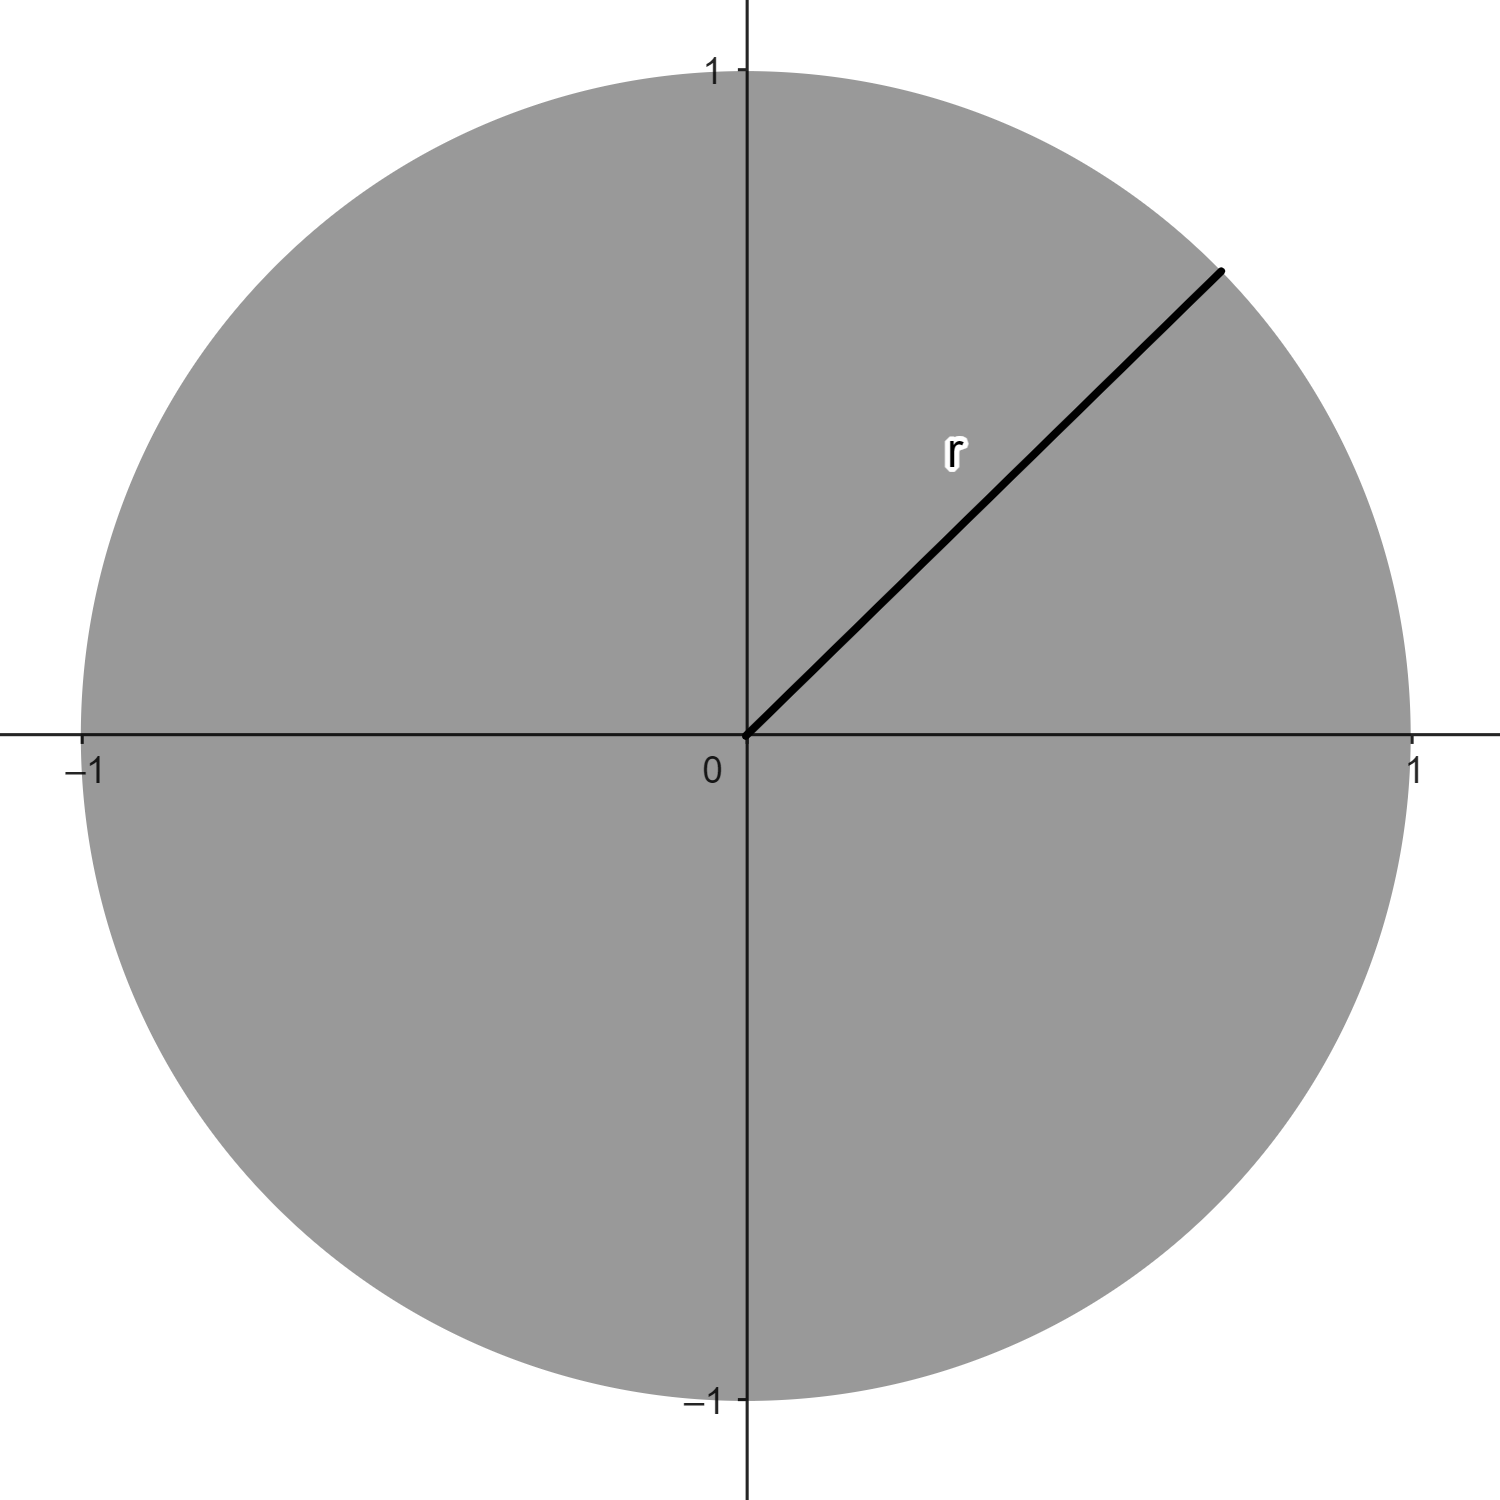
\includegraphics[width=0.75\textwidth]{Figuras/bola.png}\\
            \footnotesize{Fonte: O autor.}
            \label{fig:bola}
        \end{minipage}\hfill
        \begin{minipage}[c]{0.5\linewidth}
            \centering
            \caption{Esfera no plano.}
            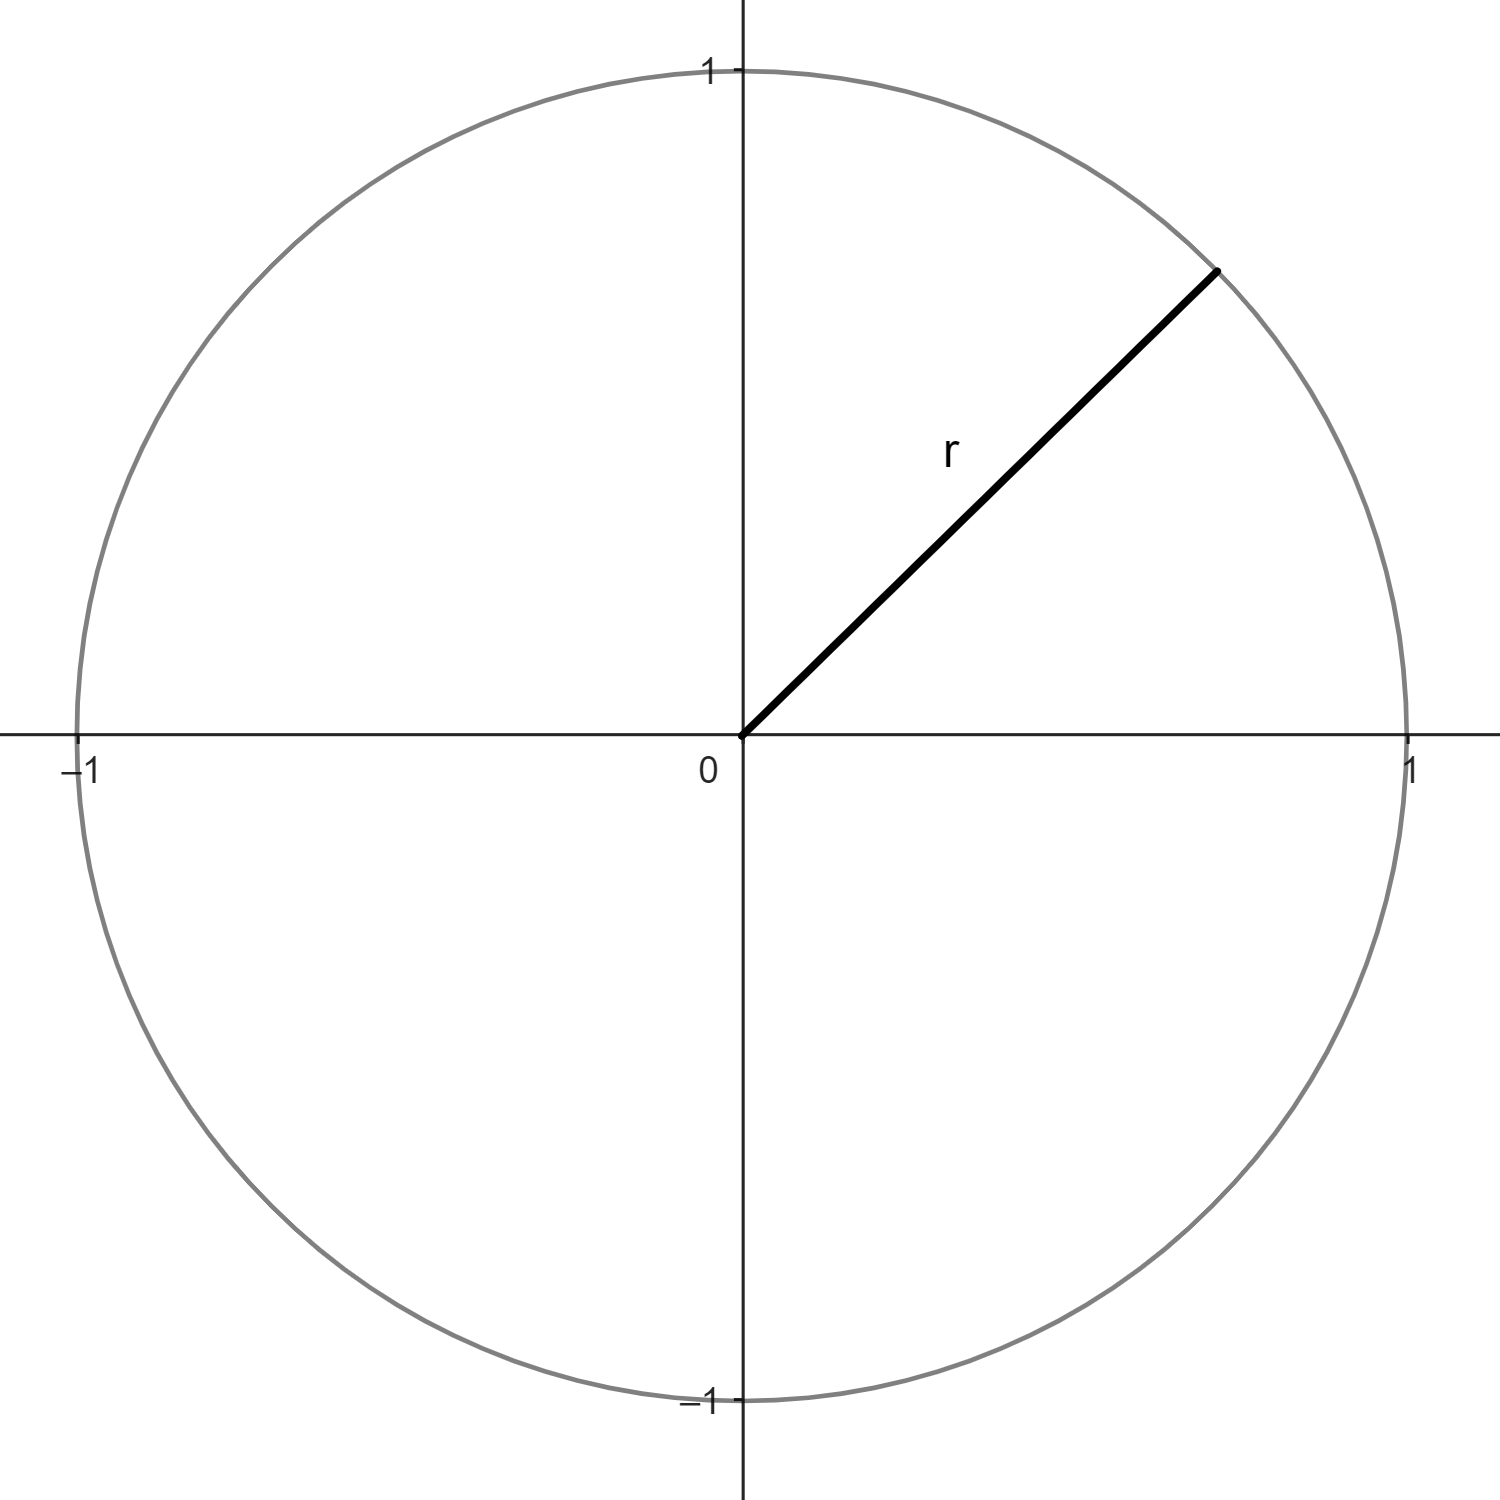
\includegraphics[width=0.75\textwidth]{Figuras/esfera.png}\\
            \footnotesize{Fonte: O autor.}
            \label{fig:esfera}
        \end{minipage}
    \end{figure}

    Seja $a$ um ponto pertencente ao espaço métrico $M$, dizemos que o ponto $a$ é um ponto isolado se $M \cap B(a,r) = \{a\}$, para algum $r > 0$, isto é, se além do próprio ponto $a$, nenhum outro ponto de $M$ está a uma distância inferior a $r$ de $a$.

    \begin{definition}[espaço métrico discreto]
        Um espaço métrico $M$ é dito discreto, se todo elemento pertencente a $M$ for isolado.
    \end{definition}
        
    \begin{exemplo}
        o espaço métrico do conjunto dos inteiros e distância euclidiana é um espaço métrico discreto, pois conseguimos definir um $r > 0$ tal que seja o raio de uma bola aberta com origem em quaisquer inteiro e que este inteiro, seja isolado. Já o conjunto $\{0,1,1/2,...,1/n\}$ não é discreto, pois o elemento 0 não é isolado para algum elemento do conjunto, ou seja, não conseguimos definir uma distância mínima entre os elementos desse conjunto.
    \qed
    \end{exemplo}

\chapter{Demonstrações}
\label{ap:demonstrações}
    Para facilitar a leitura do texto, todas as demonstrações de teoremas e isomorfismos estarão separados neste apêndice.

    \section{Teorema fundamental da aritmética}
        \begin{theorem}[teorema fundamental da aritmética]
            Todo número natural maior que 1 ou é primo, ou pode ser escrito como um produto de números primos.
        \end{theorem}
    
        \begin{proof}\ 
            \begin{enumerate}
                \item [] Por indução em $n$.
                \item \textit{base da indução}: sendo $n = 2$ e como 2 é um número primo, a base está provada.
                \item \textit{hipótese de indução}: sendo um $k \ge 2$ qualquer, supomos que todo $i = 2,3,...,k$ é primo ou um produto de primos.
                \item \textit{passo indutivo}: provar a propriedade para $k+1$. Caso $k+1$ seja número primo, a propriedade é satisfeita. Caso $k+1$ seja número composto então $k+1 = n_1 n_2$ para $1 < n_1 < k+1$ e $1 < n_2 < k+1$. Aplicando a hipótese de indução em $n_1$ e $n_2$, temos que $k+1$ é um produto de primos, satisfazendo a propriedade.
            \end{enumerate}
        \end{proof}

    \pagebreak
    \section{Isomorfismos aditivos sobre reticulados}
        Seja $\sigma_1$ e $\sigma_{1}^{-1}$ os seguintes mapeamentos entre um reticulado de base de tamanho $n$ e polinômios de grau $n-1$.
    
        \begin{center}
            $\begin{array}{rl}
                \sigma_1 &:P[x] \to \mathbb{Z}^n\\
                       &:a_1 + a_2 x + a_3 x^2 + ... + a_{n} x^{n-1} \to (a_1, a_2, a_3, ... , a_{n})
            \end{array}$\\
        
            $\begin{array}{rl}
                \sigma_1^{-1} &:\mathbb{Z}^n \to P[x]\\
                       &:(a_1, a_2, a_3, ... , a_{n}) \to a_1 + a_2 x + a_3 x^2 + ... + a_{n} x^{n-1}
            \end{array}$\\
        \end{center}
    
        Para provar que de fato $\sigma_1$ é um isomorfismo aditivo, deve-se demonstrar três propriedades:
    
        \begin{itemize}
            \item[(i)] $\sigma_1(P[x] + Q[x]) = \sigma_1(P[x]) + \sigma_1(Q[x])$,
            \item[(ii)] $\sigma_1(\sigma_1^{-1}) = \mathbb{Z}^n$ e
            \item[(ii)] $\sigma_1^{-1}(\sigma_1) = P[x]$.
        \end{itemize}
    
        Demonstração do item (i):\\
        \begin{tabular}{l}
            $\begin{array}{rl}
                 \sigma_1((a_1 + a_2 x + a_3 x^2 + ... + a_{n} x^{n-1}) + (b_1 + b_2 x + b_3 x^2 + ... + b_{n} x^{n-1}))         &= \\ \sigma_1(a_1 + a_2 x + a_3 x^2 + ... + a_{n} x^{n-1}) + \sigma_1(b_1 + b_2 x + b_3 x^2 + ... + b_{n} x^{n-1})\\\\
    
                 \sigma_1((a_1 + b_1) + (a_2 + b_2) x + (a_3 + b_3) x^2 + ... + (a_{n} + b_{n}) x^{n-1}) &=\\ \sigma_1(a_1 + a_2 x + a_3 x^2 + ... + a_{n} x^{n-1}) + \sigma_1(b_1 + b_2 x + b_3 x^2 + ... + b_{n} x^{n-1})\\\\
            
                (a_1 + b_1, a_2 + b_2, a_3 + b_3, ... , a_n + b_n) &=\\ (a_1, a_2, a_3, ... , a_n) + (b_1, b_2, b_3, ... , b_n)\\\\
            
                (a_1 + b_1, a_2 + b_2, a_3 + b_3, ... , a_n + b_n) &=\\ (a_1 + b_1, a_2 + b_2, a_3 + b_3, ... , a_n + b_n)
            
            \end{array}$
        \end{tabular}\\\\
    
        Demonstração do item (ii):\\
        \begin{tabular}{l}
            $\begin{array}{rl}
                \sigma_1(\sigma_1^{-1}(a_1, a_2, a_3, ... , a_n)) &= (a_1, a_2, a_3, ... , a_n)\\
            
                \sigma_1(a_1 + a_2 x + a_3 x^2 + ... + a_{n} x^{n-1}) &= (a_1, a_2, a_3, ... , a_n)\\
                
                (a_1, a_2, a_3, ... , a_n) &= (a_1, a_2, a_3, ... , a_n)\\
            \end{array}$
        \end{tabular}\\\\
    
        Demonstração do item (iii):\\
        \begin{tabular}{l}
            $\begin{array}{rl}
                \sigma_1^{-1}(\sigma_1(a_1 + a_2 x + a_3 x^2 + ... + a_{n} x^{n-1})) &= a_1 + a_2 x + a_3 x^2 + ... + a_{n} x^{n-1}\\
                \sigma_1^{-1}((a_1, a_2, a_3, ... , a_n)) &= a_1 + a_2 x + a_3 x^2 + ... + a_{n} x^{n-1}\\
                a_1 + a_2 x + a_3 x^2 + ... + a_{n} x^{n-1} &= a_1 + a_2 x + a_3 x^2 + ... + a_{n} x^{n-1}
            \end{array}$
        \end{tabular}\\\\
    
        Desta forma provamos que $\sigma_1$ é um isomorfismo aditivo, isto significa que $P[x]$ e $\mathbb{Z}^n$ se comportam da mesma forma com relação à operação de adição.
        Seja $\sigma_2$ e $\sigma_{2}^{-1}$ os seguintes mapeamentos entre um reticulado de base de tamanho $n$ e matrizes-linha com $n$ colunas.
    
        \begin{center}
            $\begin{array}{rl}
                    \sigma_2 &:M_n \to \mathbb{Z}^n\\
                           &:[a_1\ a_2\ a_3\ ...\ a_n] \to (a_1, a_2, a_3, ... , a_n)
            \end{array}$\\
        
            $\begin{array}{rl}
                    \sigma_2^{-1} &:\mathbb{Z}^n \to M_n\\
                           &:(a_1, a_2, a_3, ... , a_n) \to [a_1\ a_2\ a_3\ ...\ a_n]
            \end{array}$\\
        \end{center}
    
        Para provar que $\sigma_2$ é um isomorfismo aditivo, devemos garantir as mesmas três propriedades que provamos para $\sigma_1$, mas agora respeitando o domínio e contradomínio de $\sigma_2$.
    
        Demonstração do item (i):\\
        \begin{tabular}{l}
            $\begin{array}{rl}
                 \sigma_2([a_1\ a_2\ a_3\ ...\ a_n] + [b_1\ b_2\ b_3\ ...\ b_n]) &=  \sigma_2([a_1\ a_2\ a_3\ ...\ a_n]) + \sigma_2([b_1\ b_2\ b_3\ ...\ b_n])\\
                 \sigma_2([a_1 + b_1\ a_2 + b_2\ a_3 + b_3\ ...\ a_n + b_n]) &=  \sigma_2([a_1\ a_2\ a_3\ ...\ a_n]) + \sigma_2([b_1\ b_2\ b_3\ ...\ b_n])\\
                 (a_1 + b_1, a_2 + b_2, a_3 + b_3, ... , a_n + b_n) &= (a_1, a_2, a_3, ... , a_n) + (b_1, b_2, b_3, ... , b_n)\\
                 (a_1 + b_1, a_2 + b_2, a_3 + b_3, ... , a_n + b_n) &= (a_1 + b_1, a_2 + b_2, a_3 + b_3, ... , a_n + b_n)
            \end{array}$
        \end{tabular}\\\\
    
        Demonstração do item (ii):\\
        \begin{tabular}{l}
            $\begin{array}{rl}
                \sigma_2(\sigma_2^{-1}((a_1, a_2, a_3, ... , a_n))) &= (a_1, a_2, a_3, ... , a_n)\\
                \sigma_2([a_1\ a_2\ a_3\ ...\ a_n]) &= (a_1, a_2, a_3, ... , a_n)\\
                (a_1, a_2, a_3, ... , a_n) &= (a_1, a_2, a_3, ... , a_n)\\
            \end{array}$
        \end{tabular}\\\\
    
        Demonstração do item (iii):\\
        \begin{tabular}{l}
            $\begin{array}{rl}
                \sigma_2^{-1}(\sigma_2([a_1\ a_2\ a_3\ ...\ a_n])) &= {[}a_1\ a_2\ a_3\ ...\ a_n{]}\\
                \sigma_2^{-1}((a_1, a_2, a_3, ... , a_n)) &= {[}a_1\ a_2\ a_3\ ...\ a_n{]}\\
                {[}a_1\ a_2\ a_3\ ...\ a_n{]} &= {[}a_1\ a_2\ a_3\ ...\ a_n{]}\\
            \end{array}$
        \end{tabular}\\\\


\end{document}
